\documentclass[11pt,a4paper]{article}
\usepackage[utf8]{inputenc}
\usepackage[T1]{fontenc}
\usepackage{lmodern}
\usepackage[english]{babel}
\usepackage[a4paper,margin=2.3cm]{geometry}
\usepackage{graphicx}
\usepackage[section]{placeins}
\usepackage{array,longtable}
\usepackage[table]{xcolor}
\usepackage{enumitem}
\usepackage[font=small,labelfont=bf]{caption}
\usepackage{fancyhdr}
\usepackage{url}
\usepackage[hidelinks]{hyperref}
\usepackage{lastpage}

\definecolor{hdr}{HTML}{1F4E79}
\definecolor{accent}{HTML}{2E75B6}
\usepackage{soul}
\sethlcolor{yellow}
\newcommand{\tofill}[1]{\hl{TO FILL: #1}}
\setlist{itemsep=2pt,topsep=4pt}
\setlength{\parindent}{0pt}
\setlength{\parskip}{6pt}
\setcounter{tocdepth}{2}
\setlength{\LTpre}{4pt}
\setlength{\LTpost}{8pt}
\renewcommand{\arraystretch}{1.25}
\urlstyle{same}
\def\UrlBreaks{\do\/\do\_\do\-\do\.}

\pagestyle{fancy}
\fancyhf{}
\lhead{\small amaply: Software Requirements Specification}
\rhead{\small v1.0}
\lfoot{\small ENGREQ TP1 2026/2027}
\rfoot{\small Page \thepage\ of \pageref{LastPage}}
\renewcommand{\headrulewidth}{0.4pt}

\hypersetup{pdftitle={amaply - Software Requirements Specification},pdfauthor={Joana Rocha, Bendik Halstensen, Rodrigo Monteiro}}

\begin{document}

\begin{titlepage}
\centering
\vspace*{2cm}
{\large ISEP, Master's in Informatics Engineering\par}
{\large Requirements Engineering (ENGREQ), Practical Assignment No. 1\par}
\vspace{3cm}
{\Huge\bfseries\color{hdr} amaply\par}
\vspace{0.6cm}
{\LARGE Software Requirements Specification\par}
\vspace{0.3cm}
{\large Version 1.0\par}
\vspace{3cm}
{\large Joana Rocha (1211652)\par}
\vspace{0.15cm}
{\large Bendik Halstensen (1260122)\par}
\vspace{0.15cm}
{\large Rodrigo Monteiro (1260551)\par}
\vspace{0.3cm}
{\large 2026/2027\par}
\vfill
{\small Repository: \url{https://github.com/joanarcrocha/enreq-amaply}\par}
\end{titlepage}

\section*{Revision history}
{\footnotesize
\begin{longtable}{>{\raggedright\arraybackslash}p{1.5cm}>{\raggedright\arraybackslash}p{3.5cm}>{\raggedright\arraybackslash}p{7.2cm}>{\raggedright\arraybackslash}p{2.3cm}}
\rowcolor{hdr}\textcolor{white}{\textbf{Version}} & \textcolor{white}{\textbf{Author}} & \textcolor{white}{\textbf{Description}} & \textcolor{white}{\textbf{Date}} \\
1.0 & J. Rocha, B. Halstensen, R. Monteiro & Initial version, built from the elicitation evidence in the project repository & 2026-11-09 \\ \hline
\end{longtable}}
\addtocounter{table}{-1}

\tableofcontents
\clearpage

\section{Introduction}


\subsection{Purpose}

This document specifies the software requirements of \textbf{amaply}, release 1.0. amaply is the name the team gave to the platform referred to as FAIR-AMAP in the assignment statement [A]: a web platform, promoted by FAIR Software Solutions, that supports the operation of AMAP/CSA communities (groups of consumers, called co-producers, who directly support one or more local farmers).

The document is intended for the following readers:

\begin{itemize}
  \item \textbf{FAIR Software Solutions management}, to validate that the scope matches the business opportunity;
  \item \textbf{Stakeholder representatives} (producers, co-producers and AMAP coordinators), to confirm that their needs were understood;
  \item \textbf{Development team and architects}, as the basis for design, implementation and estimation;
  \item \textbf{Testers}, to derive acceptance tests from each verifiable requirement;
  \item \textbf{ENGREQ lecturers}, to assess the specification and the elicitation process that produced it (section 10).
\end{itemize}
The system does not exist yet, so the text describes what it should do. Sections 1.3, 2.2 and 3.1 give the short version: what the product is for, who uses it and what they do with it. Section 5 defines the vocabulary used everywhere else.


\subsection{Document conventions}

\begin{itemize}
  \item The structure follows the SRS outline of Wiegers and Beatty, Software Requirements (3rd ed.), aligned with ISO/IEC/IEEE 29148 and extended with the elements required by the assignment (estimates per functionality and description of the process).
  \item Functional requirements are identified as \textbf{FR-nn}, quality requirements as \textbf{NFR-xx-nn} (U usability, P performance, S security, SF safety, O others), localization requirements as \textbf{LOC-nn}, data rules as \textbf{DR-nn}, reports as \textbf{REP-nn}, user interface views and rules as \textbf{UI-nn} and communication rules as \textbf{COM-nn} and other requirements as \textbf{OR-nn}. User stories in the backlog are \textbf{US-nn}.
  \item Priorities follow the MoSCoW scale: \textbf{Must} (release 1.0 cannot go live without it), \textbf{Should} (important, planned for release 1.0 but can slip), \textbf{Could} (desirable, only if capacity allows), \textbf{Won't (this release)}. In the backlog, Must = 1, Should = 2, Could = 3.
  \item Every requirement states its \textbf{source} and a \textbf{justification}, following the project rule that all information must be documented and justified. Source codes are listed in Table 1.
  \item \textbf{Requirement language.} ``Shall'' marks a mandatory requirement, ``should'' a desirable one and ``may'' an option.
  \item \textbf{Use cases} are UC01 to UC14 (section 3.1). Diagrams follow UML 2; the domain models are conceptual, so their attributes are examples and not a database design.
  \item \textbf{Terms.} A co-producer is a member of an AMAP or CSA who pays for a season in advance and shares its risk. A share is what a co-producer commits to for the whole season. A basket is what the share yields on one distribution day. Other terms are in the glossary (Appendix 12.1).
  \item Text highlighted in yellow and marked TO FILL is data that the team still has to supply (dates, effort hours); it was left open on purpose instead of being invented.
  \item Requirements derived by the analyst (source AN) and values that depend on open questions are marked ``to be validated'' and are listed in section 2.5.
\end{itemize}
{\footnotesize
\begin{longtable}{>{\raggedright\arraybackslash\hspace{0pt}}p{\dimexpr 0.103\linewidth-2\tabcolsep\relax}>{\raggedright\arraybackslash\hspace{0pt}}p{\dimexpr 0.479\linewidth-2\tabcolsep\relax}>{\raggedright\arraybackslash\hspace{0pt}}p{\dimexpr 0.418\linewidth-2\tabcolsep\relax}}
\caption{Source codes used for traceability}\\
\rowcolor{hdr}\textcolor{white}{\textbf{Code}} & \textcolor{white}{\textbf{Meaning}} & \textcolor{white}{\textbf{Evidence in the repository}} \\ \endfirsthead
\rowcolor{hdr}\textcolor{white}{\textbf{Code}} & \textcolor{white}{\textbf{Meaning}} & \textcolor{white}{\textbf{Evidence in the repository}} \\ \endhead
A & Assignment statement (FAIR-AMAP, ENGREQ TP1 2026/2027) & \url{docs/assignment/engreq_tp1_2026_27_v2_EN.pdf} \\ \hline
S1-Qn & Elicitation session 1 (interview with stakeholders), question n (Q1 to Q10) & \url{docs/elicitation/session-notes.en.md} \\ \hline
S2-Pn & Elicitation session 2 (structured interview), producer question n & \url{docs/elicitation/ENGREQ_Interview_Questions_and_Answers.md} \\ \hline
S2-Cn & Elicitation session 2, co-producer question n & \url{docs/elicitation/ENGREQ_Interview_Questions_and_Answers.md} \\ \hline
S2-F & Elicitation session 2, additional findings & \url{docs/elicitation/ENGREQ_Interview_Questions_and_Answers.md} \\ \hline
OQ & Open question or point still to confirm with stakeholders & \url{docs/elicitation/open-questions.en.md} \\ \hline
IN-P & Supplementary interview notes, producer (Biogoods AMAP) & \url{docsoldgroup/notas-entrevistas/notas-entrevista-biogoods-amap.md} \\ \hline
IN-C & Supplementary interview notes, co-producer & \url{docsoldgroup/notas-entrevistas/notas-entrevista-coprodutor-Luisa-Marques.md} \\ \hline
MR & Desk research by Rodrigo Monteiro: market and software review, personas and process maps & Findings summarised in this document \\ \hline
AN & Analyst derivation: inferred from the sources above, from legal context or from domain practice; justification given and validation pending & This document \\ \hline
\end{longtable}}

\subsection{Project scope}

FAIR Software Solutions is a startup that develops software to facilitate the distribution and sale of food products, aligned with the UN 2030 Agenda and its 17 Sustainable Development Goals [A]. The company identified a business opportunity in the AMAP/CSA field [A]. In the first session the stakeholders stated that the goal is \textbf{not to create CSAs} but to \textbf{streamline the existing process and energise the CSA market}, monetising through a CSA portal with an international ambition, since Portugal has only a few dozen CSAs [S1-Q6].

amaply addresses two main needs expressed by the stakeholders [S1-Q1]: \textbf{communication} between producers and co-producers, and \textbf{simpler payment processes}. To do so, release 1.0 covers:

\begin{itemize}
  \item discovery of AMAPs by location and exploration of their offers before joining [S1-Q5, S2-F];
  \item membership management, admission by the AMAP management and waiting lists [S1-Q5, S2-P4];
  \item producer offers (seasonal baskets and individual products) and co-producer subscriptions [S1-Q2, S2-C2];
  \item delivery calendar, collection points, notifications and absence arrangements [S1-Q4, S2-P5];
  \item handling of shortages through replacement, refund or platform credit, and seasonal balance tracking [S2-P2, S1-Q7];
  \item a single combined payment per co-producer, in instalments, with funds reaching producers before delivery [S2-P1, S2-C1];
  \item invoicing adapted to the legal setup of each AMAP [S1-Q10];
  \item news, chat and notifications [S1-Q7, S2-C3];
  \item producer certificates and optional sustainability indicators [S1-Q9].
\end{itemize}
\textbf{Business objectives.} BO-1: reduce the administrative effort of running an AMAP (payments, deliveries, communication). BO-2: make AMAPs easier to find and join, increasing the number of co-producers per AMAP. BO-3: generate revenue through a small fee per transaction, compatible with the AMAP spirit that rejects predatory commissions [S1-Q3]. BO-4: contribute to the SDGs (poverty reduction, sustainable communities, protection of natural resources) [S1-Q9].

The desk research adds a view of current practice and further aims [MR]. In an AMAP or CSA, a group of co-producers pays a farmer in advance for a season and shares the harvest, good or bad. From the sources reviewed, most groups in Portugal and Spain run this on shared spreadsheets, chat groups, e-mail and manual checks of bank transfers. Producers do the accounts after a day in the field. A co-producer who goes on holiday either loses a basket or has to write to someone about it. How common this is still has to be confirmed. The resulting objectives are:

\begin{itemize}
  \item \textbf{BO-5} give producers an early view of their income and of what to harvest [MR];
  \item \textbf{BO-6} lose fewer baskets, by making absences easy to report and to redirect [MR, S2-P5];
  \item \textbf{BO-7} work on a phone, with weak coverage, using Portuguese payment methods, language and tax rules [MR].
\end{itemize}
The product relates to SDG 2 (targets 2.3 and 2.4), SDG 11 (target 11.a) and SDG 12 (target 12.3): income for small producers, links between city and countryside, and less food waste [R5, MR]. FAIR has not decided on pricing; the market research suggests that percentage commissions on food sales would not be accepted by this community [MR], which agrees with S1-Q3.

\textbf{Out of scope for release 1.0} (with justification):

\begin{itemize}
  \item Creating new AMAPs from scratch as a service or recruiting farmers: the stakeholders said the focus is not to create CSAs [S1-Q6].
  \item Managing uncollected baskets beyond recording them: the producer said the platform does not need to manage them [S2-P5].
  \item A formal dispute resolution process: co-producers prefer informal resolution based on trust, supported by chat and AMAP management [S2-C3].
  \item Logistics and transport management between farm and collection point: no stakeholder mentioned it; producers drop off at a fixed point [S1-Q4].
  \item Communication between different AMAPs: mentioned as possible but ``not necessarily required'' [S2-F]; kept as a Could requirement (FR-53).
  \item Online sales to the general public, home delivery and crop planning beyond the weekly harvest [MR]: the core model is the season commitment collected at fixed pickup points (AS-10, AS-11).
  \item Payment processing and certified invoicing themselves: left to a payment provider and to existing invoicing software (CO-2, CO-3) [MR].
\end{itemize}

\subsection{References}

\begin{itemize}
  \item [A] Santos, J. and Silva, B. (2026). ENGREQ Practical Assignment No. 1, FAIR-AMAP, version 1.0. ISEP, Master's in Informatics Engineering.
  \item [R1] Project repository: \url{https://github.com/joanarcrocha/enreq-amaply} (elicitation notes, open questions, planning and session log).
  \item [R2] Wiegers, K. and Beatty, J. (2013). Software Requirements, 3rd edition. Microsoft Press.
  \item [R3] ISO/IEC/IEEE 29148:2018. Systems and software engineering, Life cycle processes, Requirements engineering.
  \item [R4] AMAP movement in Portugal: \url{https://amap.movingcause.org/} (referenced in the assignment).
  \item [R5] United Nations Sustainable Development Goals (Portuguese portal): \url{https://ods.pt/ods/}
  \item [R6] Regulation (EU) 2016/679, General Data Protection Regulation (GDPR).
  \item [R7] W3C (2018). Web Content Accessibility Guidelines (WCAG) 2.1.
  \item [R8] Regulation (EU) No 1169/2011 on the provision of food information to consumers.
  \item [R9] URGENCI (2016). Overview of Community Supported Agriculture in Europe. \url{https://urgenci.net/}
  \item [R10] PROVE, Promover e Vender (Portuguese network of short food chains). \url{https://www.prove.com.pt/}
  \item [R11] Websites of the software reviewed in the desk research: AmapJ, Cagette.net, OpenOlitor, Open Food Network, Harvie, Barn2Door, Farmigo, LocalLine and others.
\end{itemize}

\section{Overall description}


\subsection{Product perspective}

amaply is a \textbf{new, self-contained product}. It does not replace an existing FAIR system. Today, according to the sessions, AMAPs operate with direct contact between producers and co-producers, payments by MB Way or bank transfer made separately to each producer, and information spread over informal channels [S2-C1, S1-Q10]. The international CSA web page only suggests the nearest CSA, and the joining process continues outside it [S1-Q5]. amaply brings these steps into a single platform.

Figure 1 shows the system context. On the left are the user classes described in section 2.2; on the right, the external systems amaply depends on. The figure shows that money and invoices are handled through external specialised services, which keeps the platform from holding funds (FR-42) and from issuing tax documents itself (FR-49).

\begin{figure}[htbp]\centering
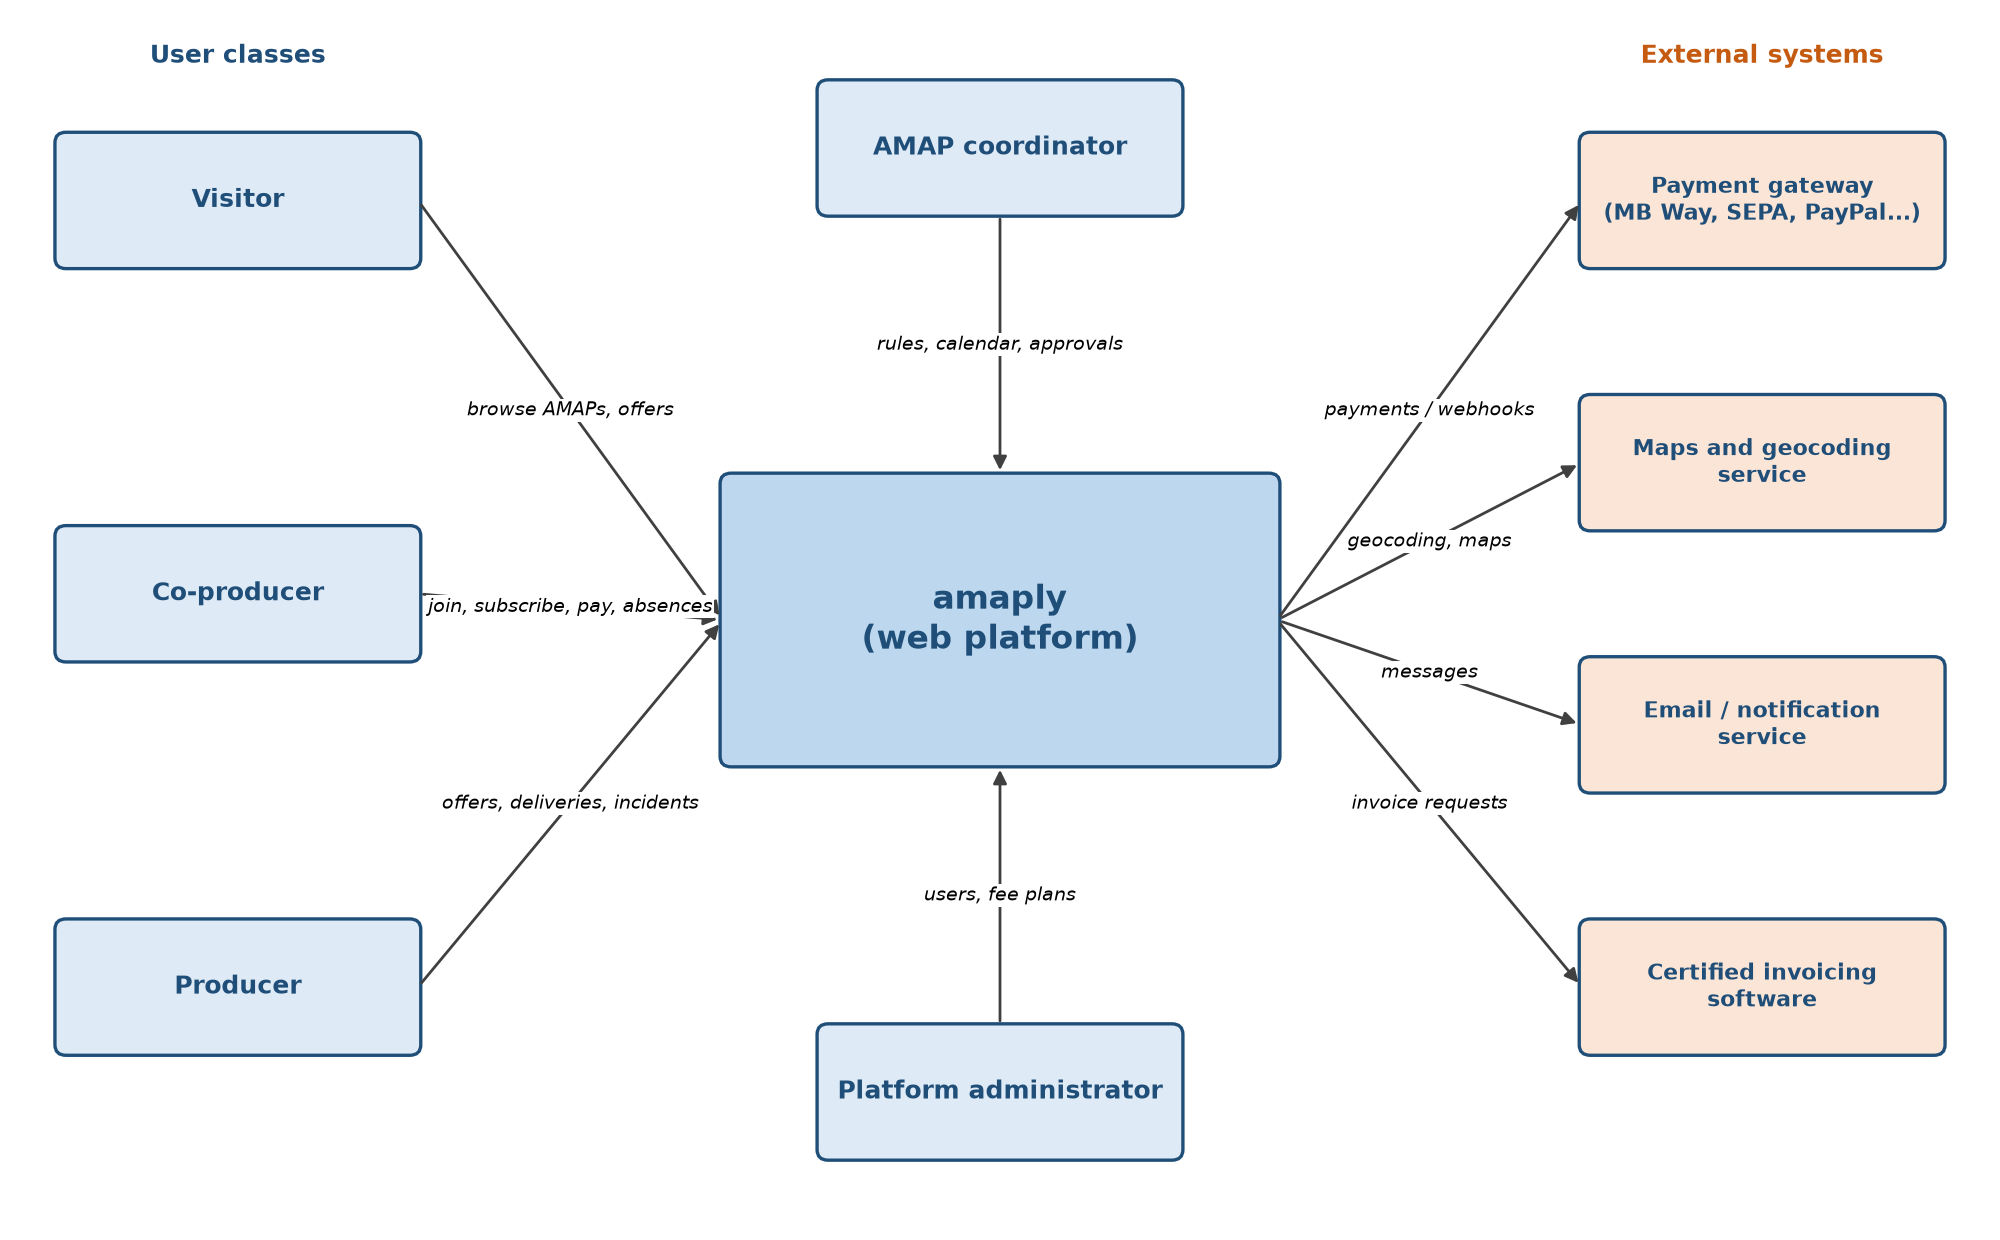
\includegraphics[width=0.94\linewidth]{figures/fig1_context.png}
\caption{amaply context diagram (user classes and external systems)}\label{fig:fig1_context}
\end{figure}
What amaply displaces is the set of informal tools described in section 1.3, which cost nothing and which everyone already knows how to use [MR]. Existing software falls into two groups [R11]. AmapJ, OpenOlitor and Open Food Network are open source or non-profit, and free or cheap. Farmigo, LocalLine, Harvie and Barn2Door are commercial, mostly North American, and charge a monthly fee or a share of sales. Few of them could be tried, so this comes from what each vendor says on its own site. None of those sites mentions Portuguese payment methods, the Portuguese language or Portuguese tax rules. PROVE [R10], the Portuguese network of short food chains, is context and not a software competitor.

Users reach amaply through a web and mobile app (Figure \ref{fig:fig1_context}). Producers and AMAP coordinators need an offline mode, because farms and some collection points have no reliable coverage (OE-5). Payments, receipts and notifications go through external services, and the technology is left to design.

\subsection{User classes and characteristics}

User classes are a subset of the stakeholders identified in section 10.1. The two favoured classes, whose satisfaction determines the success of the product, are \textbf{producers} and \textbf{co-producers} (README, stakeholder definition).

{\footnotesize
\begin{longtable}{>{\raggedright\arraybackslash\hspace{0pt}}p{\dimexpr 0.145\linewidth-2\tabcolsep\relax}>{\raggedright\arraybackslash\hspace{0pt}}p{\dimexpr 0.436\linewidth-2\tabcolsep\relax}>{\raggedright\arraybackslash\hspace{0pt}}p{\dimexpr 0.145\linewidth-2\tabcolsep\relax}>{\raggedright\arraybackslash\hspace{0pt}}p{\dimexpr 0.109\linewidth-2\tabcolsep\relax}>{\raggedright\arraybackslash\hspace{0pt}}p{\dimexpr 0.164\linewidth-2\tabcolsep\relax}}
\caption{User classes}\\
\rowcolor{hdr}\textcolor{white}{\textbf{User class}} & \textcolor{white}{\textbf{Description and characteristics}} & \textcolor{white}{\textbf{Frequency of use}} & \textcolor{white}{\textbf{Importance}} & \textcolor{white}{\textbf{Source}} \\ \endfirsthead
\rowcolor{hdr}\textcolor{white}{\textbf{User class}} & \textcolor{white}{\textbf{Description and characteristics}} & \textcolor{white}{\textbf{Frequency of use}} & \textcolor{white}{\textbf{Importance}} & \textcolor{white}{\textbf{Source}} \\ \endhead
Co-producer & Consumer who supports one or more producers by subscribing to their production. Two profiles: ``organic'' (motivated by the food) and ``ideological'' (motivated by working directly with farmers). Can belong to several AMAPs. Mostly non-technical, uses a smartphone. & Weekly (collection) and per payment cycle & Favoured & S1-Q1, S1-Q6, S2-C4 \\ \hline
Producer & Farmer or food producer (vegetables, wine, eggs, bread, etc.) who creates offers and delivers produce. Limited time, often in the field, variable digital literacy. Needs money before delivery to finance production. & Several times per week in season & Favoured & S1-Q2, S2-P1 \\ \hline
AMAP coordinator & Person or team from the AMAP management. Admits members, defines the delivery calendar, approves pauses and cancellations and configures the AMAP rules. Described as an important actor. & Weekly & High & S1-Q7, S2-P3, S2-P4 \\ \hline
Visitor & Person without an account who explores AMAPs and their offers before deciding to join. & Occasional & Medium & S2-C4, S2-F \\ \hline
Platform administrator & FAIR Software Solutions staff who manage accounts, fee plans and platform settings. & Daily & Medium & AN (needed to operate the monetisation model of S1-Q3) \\ \hline
\end{longtable}}
A single person may hold several roles, for example a producer who is also a co-producer of another AMAP. The producer interviewed said this ``does not matter'' to them [S2-P6]; the draft allows it (FR-02) to avoid duplicate accounts. This is an analyst decision informed by S2-P6, rather than an explicit stakeholder requirement.

The AMAP coordinator is not necessarily a separate person: one account can hold several roles (FR-02), so a co-producer can also be the coordinator. Two other groups appear occasionally and have no account: people who collect a basket for a co-producer, and institutions that receive donated baskets [MR, S2-P5].


\subsection{Operating environment}

\begin{itemize}
  \item \textbf{OE-1} amaply is a web application accessed through current versions of Chrome, Edge, Firefox and Safari, on desktop and on smartphones (Android and iOS). Justification: co-producers check collection details on the move and producers work in the field (AN, from S1-Q4 and S1-Q2).
  \item \textbf{OE-2} The server side runs on a cloud infrastructure with data stored in data centres located in the European Union. Justification: the first users are Portuguese and GDPR [R6] restricts transfers of personal data outside the EU (AN).
  \item \textbf{OE-3} The system must coexist with the payment gateway, maps service, email service and certified invoicing software described in section 6.2.
  \item \textbf{OE-4} Users are initially located in Portugal; the solution must be ready for other countries since it is meant to be international [S1-Q6]. Spain is a likely second market [MR].
  \item \textbf{OE-5} Producer and AMAP coordinator functions work offline and synchronise later, because farms and some pickup points have no reliable coverage [MR].
  \item \textbf{OE-6} The platform sends notifications by e-mail, SMS and push, and exchanges data with payment providers, invoicing software and spreadsheets (CSV) [MR]. SMS and push go beyond the channels assumed for launch (AS-04) and are to be validated.
\end{itemize}

\subsection{Design and implementation constraints}

\begin{itemize}
  \item \textbf{CO-1 Personal data protection.} The system processes personal data of EU citizens and must comply with GDPR [R6]. Names, addresses and consumption history may not be used for advertising or sold. Source: AN (legal), MR.
  \item \textbf{CO-2 No custody of funds.} Producers need access to the money before delivery and the platform must not hold payments [S2-P1]. Collecting and redistributing money on behalf of others is a regulated payment activity, so payments must be processed by a licensed payment provider offering split or marketplace payments. Source: S2-P1 and AN (legal).
  \item \textbf{CO-3 Invoicing law.} Who issues the invoice depends on the legal setup of each AMAP [S1-Q10]. In Portugal invoices must be issued by software certified by the Tax Authority (AT); amaply must therefore integrate with certified invoicing software rather than issue invoices itself (SAF-T). What each producer has to issue depends on their tax status, which is not yet confirmed. Source: S1-Q10, AN (legal, to be validated), MR.
  \item \textbf{CO-4 Configurability.} There are several types of AMAP with distinct rules [S1-Q2]; rules must be configuration, not code (see NFR-O-02).
  \item \textbf{CO-5 Low operating cost.} The platform must support small producers, possibly starting free or with a very small fee [S1-Q3]; technology choices must keep the cost per AMAP low.
  \item \textbf{CO-6 Languages.} Portuguese (European variant) and English at launch [S2-C6, MR].
  \item \textbf{CO-7 Payment methods.} Payments support MB WAY, Multibanco references, SEPA direct debit and bank transfer; card data is handled only by the payment provider [MR, S2-C1].
  \item \textbf{CO-8 Business model.} The business model cannot depend on a percentage of the value of baskets [MR, S1-Q3].
  \item \textbf{CO-9 Devices and connectivity.} The system runs on mid-range smartphones over mobile data, and tolerates loss of connection in the field and at pickup points [MR].
\end{itemize}

\subsection{Assumptions and dependencies}

The following assumptions are not confirmed facts. If any of them is wrong, the related requirements must be reviewed. Most come from the open questions recorded in the repository.

{\footnotesize
\begin{longtable}{>{\raggedright\arraybackslash\hspace{0pt}}p{\dimexpr 0.085\linewidth-2\tabcolsep\relax}>{\raggedright\arraybackslash\hspace{0pt}}p{\dimexpr 0.521\linewidth-2\tabcolsep\relax}>{\raggedright\arraybackslash\hspace{0pt}}p{\dimexpr 0.182\linewidth-2\tabcolsep\relax}>{\raggedright\arraybackslash\hspace{0pt}}p{\dimexpr 0.212\linewidth-2\tabcolsep\relax}}
\caption{Assumptions and dependencies}\\
\rowcolor{hdr}\textcolor{white}{\textbf{ID}} & \textcolor{white}{\textbf{Assumption or dependency}} & \textcolor{white}{\textbf{Affected requirements}} & \textcolor{white}{\textbf{Source}} \\ \endfirsthead
\rowcolor{hdr}\textcolor{white}{\textbf{ID}} & \textcolor{white}{\textbf{Assumption or dependency}} & \textcolor{white}{\textbf{Affected requirements}} & \textcolor{white}{\textbf{Source}} \\ \endhead
AS-01 & Next season's production is planned by the producer and agreed with the co-producers. & FR-21 & S1-Q2, OQ \\ \hline
AS-02 & Waiting lists are ordered by request date unless the AMAP configures another rule (no priority rule was given). & FR-13 & S1-Q5, S2-P4, S2-C4 \\ \hline
AS-03 & EUR is the only currency needed at launch (no currency was named; first users are in Portugal). & LOC-10 & S2-P6, S2-C6 \\ \hline
AS-04 & Email and in-app notifications are sufficient channels at launch (no channel was specified). & FR-54 & S2-P5 \\ \hline
AS-05 & First-year volume: up to 500 AMAPs, 50 000 registered users and 1 000 simultaneous users. Order of magnitude only, chosen because Portugal has a few dozen CSAs but the product is international. & NFR-P-02 & S1-Q6, OQ \\ \hline
AS-06 & Renewal of subscriptions happens per season, by invitation before the season ends (no renewal procedure was given). & FR-27 & S2-P3, S2-C3 \\ \hline
AS-07 & A payment provider offering MB Way, SEPA transfers and split payments to several beneficiaries is available in Portugal; support for recurring payments is still to be confirmed. & FR-40 to FR-44 & AN, MR \\ \hline
AS-08 & Each AMAP has at least one person willing to act as coordinator. & Features 3.4 and 3.5 & S1-Q7, S2-P4 \\ \hline
AS-09 & Shortages caused by quality problems are handled with the same options as missing products (no procedure was described). & FR-36 & S2-P2 \\ \hline
AS-10 & The core model is the season commitment; one-off purchases are not the aim. & Features 3.6, 3.7 & MR, S1-Q1 \\ \hline
AS-11 & Baskets are collected at fixed pickup points, on a fixed weekday and within a time window; there is no home delivery. & FR-09, FR-29 & MR, S1-Q4 \\ \hline
AS-12 & Most producers have a smartphone and will use it for data entry if the interface is simple. & NFR-U-01, NFR-U-03 & MR \\ \hline
AS-13 & A cut-off for absences is configurable per AMAP. The interviews did not mention one, so it is a proposal to confirm with real groups. Refunds, credits and replacements after a crop loss follow the producer's choice (FR-36, S2-P2). & FR-16, FR-32, FR-36 & MR, S2-P2 \\ \hline
AS-14 & Invoicing software that complies with Autoridade Tributária rules is reachable by export or API. & FR-49 & MR, CO-3 \\ \hline
AS-15 & Access to real stakeholders is limited: the FAIR director attends only the initial presentation, so most sessions are with lecturers playing roles. & Section 10 & A, MR \\ \hline
AS-16 & FAIR decides on pricing and on whether any part of the product will be open source. & FR-47 & MR \\ \hline
\end{longtable}}

\section{System features}

Section 3.1 gives an overview of the use cases. Sections 3.2 to 3.14 then group the functional requirements into 13 features, one per major service of the platform. The grouping follows the life cycle of an AMAP subscription (discover, join, subscribe, collect, pay, communicate) because this was the order in which stakeholders described their process in session 1 (questions 2, 4 and 5). Table \ref{tab:features} summarises the features and their priority.

{\footnotesize
\begin{longtable}{>{\raggedright\arraybackslash\hspace{0pt}}p{\dimexpr 0.125\linewidth-2\tabcolsep\relax}>{\raggedright\arraybackslash\hspace{0pt}}p{\dimexpr 0.625\linewidth-2\tabcolsep\relax}>{\raggedright\arraybackslash\hspace{0pt}}p{\dimexpr 0.250\linewidth-2\tabcolsep\relax}}
\caption{Summary of system features}\label{tab:features}\\
\rowcolor{hdr}\textcolor{white}{\textbf{Section}} & \textcolor{white}{\textbf{Feature}} & \textcolor{white}{\textbf{Priority}} \\ \endfirsthead
\rowcolor{hdr}\textcolor{white}{\textbf{Section}} & \textcolor{white}{\textbf{Feature}} & \textcolor{white}{\textbf{Priority}} \\ \endhead
3.2 & Accounts, roles and profiles & Must \\ \hline
3.3 & AMAP discovery and exploration & Must \\ \hline
3.4 & Membership and waiting list & Must \\ \hline
3.5 & AMAP configuration and calendar & Must \\ \hline
3.6 & Offers and products & Must \\ \hline
3.7 & Subscriptions & Must \\ \hline
3.8 & Deliveries and collection & Must \\ \hline
3.9 & Shortages and seasonal balance & Must \\ \hline
3.10 & Payments and platform fee & Must \\ \hline
3.11 & Invoicing & Should \\ \hline
3.12 & Communication and notifications & Must \\ \hline
3.13 & Sustainability indicators & Could \\ \hline
3.14 & Platform administration & Must \\ \hline
\end{longtable}}

\subsection{Use case overview}

This section, written by Rodrigo Monteiro, lists what users do with the system before the detail. The use cases come from personas and from the processes mapped in the desk research: season launch, weekly planning, distribution day, absences and crop losses [MR]. They are candidates, and some may merge or disappear after validation. Table \ref{tab:actors} lists the actors and Figure \ref{fig:rodrigo-use-cases} shows the use cases. The AMAP coordinator is the management of the AMAP and can also be a co-producer. The payment provider is an external system.

{\footnotesize
\begin{longtable}{>{\raggedright\arraybackslash\hspace{0pt}}p{\dimexpr 0.273\linewidth-2\tabcolsep\relax}>{\raggedright\arraybackslash\hspace{0pt}}p{\dimexpr 0.727\linewidth-2\tabcolsep\relax}}
\caption{Use case actors}\label{tab:actors}\\
\rowcolor{hdr}\textcolor{white}{\textbf{Actor}} & \textcolor{white}{\textbf{Role}} \\ \endfirsthead
\rowcolor{hdr}\textcolor{white}{\textbf{Actor}} & \textcolor{white}{\textbf{Role}} \\ \endhead
Producer & Runs seasons for a farm, plans harvests, follows payments and reports crop losses. \\ \hline
Co-producer & Subscribes to a season, pays, receives baskets and reports absences. \\ \hline
AMAP coordinator & Manages the AMAP: its pickup points, calendar and rules, and distribution day. \\ \hline
Platform administrator & Manages groups and users and reads aggregated impact data. \\ \hline
Payment provider (system) & Carries out and confirms payments. \\ \hline
\end{longtable}}
\begin{figure}[htbp]\centering
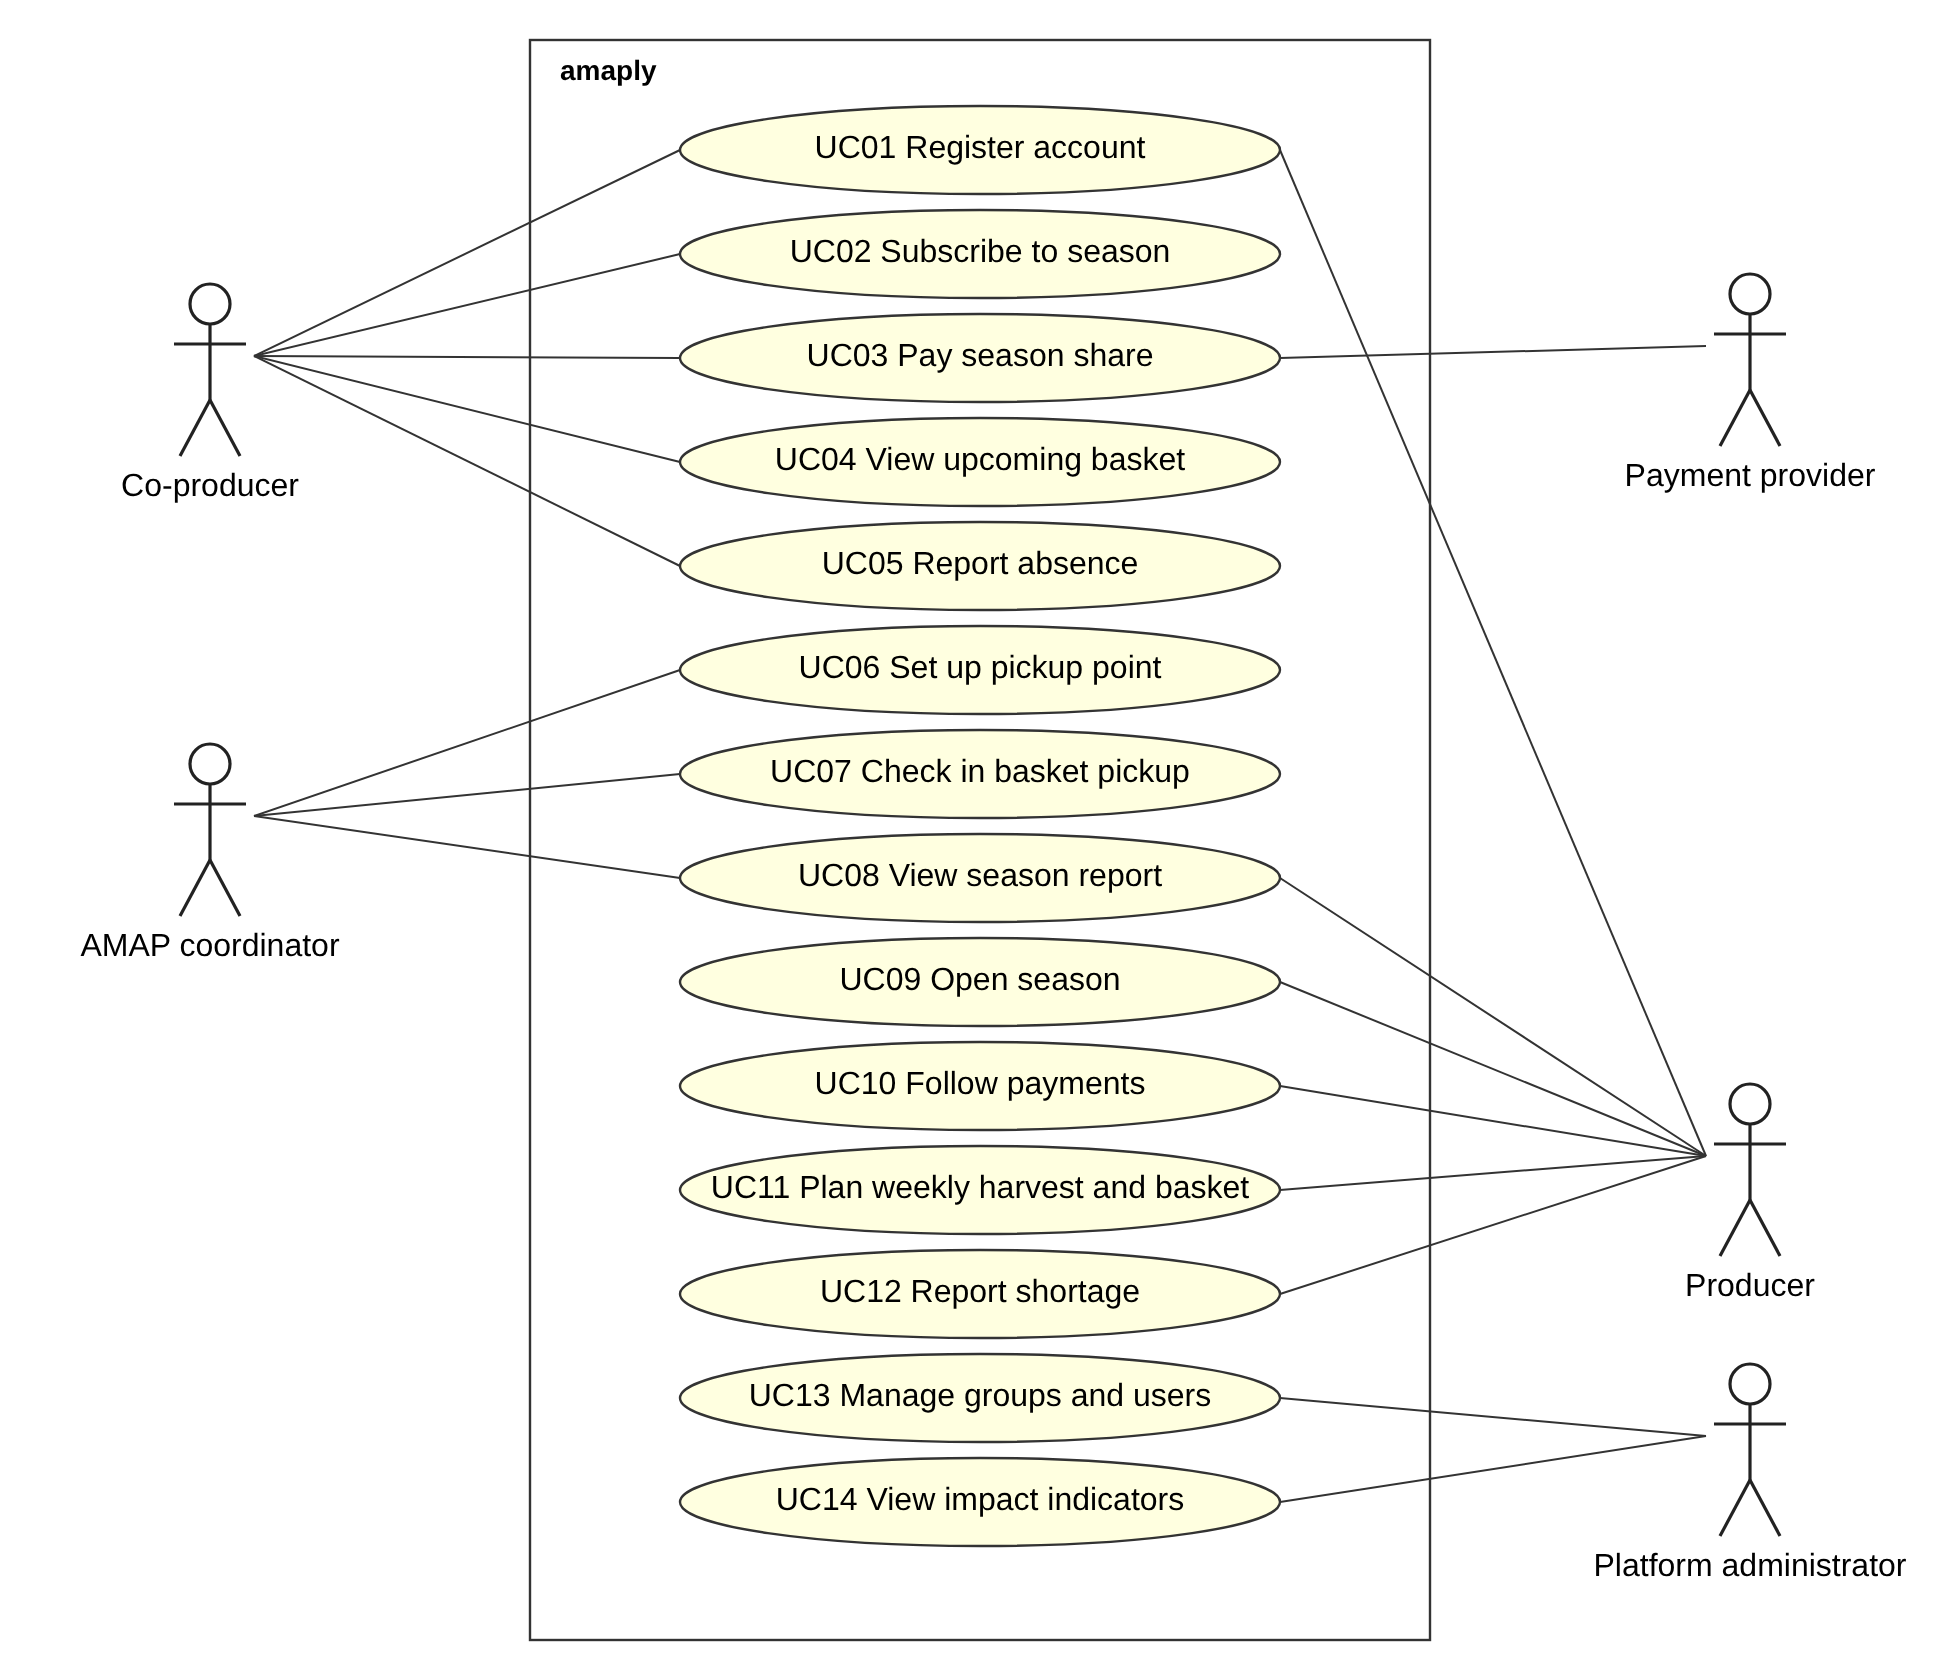
\includegraphics[width=0.79\linewidth]{figures/rodrigo-use-cases.png}
\caption{Use case diagram (R. Monteiro)}\label{fig:rodrigo-use-cases}
\end{figure}
Table \ref{tab:usecases} is the catalogue. Its High/Medium/Low priorities are provisional. The last column, added when merging, links each use case to the functional requirements of sections 3.2 to 3.14; use cases without a match, or that go beyond what the interviews asked for, are marked for validation.

{\footnotesize
\begin{longtable}{>{\raggedright\arraybackslash\hspace{0pt}}p{\dimexpr 0.096\linewidth-2\tabcolsep\relax}>{\raggedright\arraybackslash\hspace{0pt}}p{\dimexpr 0.162\linewidth-2\tabcolsep\relax}>{\raggedright\arraybackslash\hspace{0pt}}p{\dimexpr 0.150\linewidth-2\tabcolsep\relax}>{\raggedright\arraybackslash\hspace{0pt}}p{\dimexpr 0.311\linewidth-2\tabcolsep\relax}>{\raggedright\arraybackslash\hspace{0pt}}p{\dimexpr 0.102\linewidth-2\tabcolsep\relax}>{\raggedright\arraybackslash\hspace{0pt}}p{\dimexpr 0.180\linewidth-2\tabcolsep\relax}}
\caption{Use case catalogue}\label{tab:usecases}\\
\rowcolor{hdr}\textcolor{white}{\textbf{ID}} & \textcolor{white}{\textbf{Use case}} & \textcolor{white}{\textbf{Actor}} & \textcolor{white}{\textbf{Summary}} & \textcolor{white}{\textbf{Prio.}} & \textcolor{white}{\textbf{Related FR}} \\ \endfirsthead
\rowcolor{hdr}\textcolor{white}{\textbf{ID}} & \textcolor{white}{\textbf{Use case}} & \textcolor{white}{\textbf{Actor}} & \textcolor{white}{\textbf{Summary}} & \textcolor{white}{\textbf{Prio.}} & \textcolor{white}{\textbf{Related FR}} \\ \endhead
UC01 & Register account & Producer, co-producer & Create an account and join a group. Producers also register their farm and how they produce. & High & FR-01, FR-02, FR-05, FR-10 \\ \hline
UC02 & Subscribe to season & Co-producer & Choose a share and a pickup point and accept the group's charter. & High & FR-24 \\ \hline
UC03 & Pay season share & Co-producer & Pay in full or by scheduled instalments. & High & FR-40 to FR-44 \\ \hline
UC04 & View upcoming basket & Co-producer & See what the next basket holds. & Medium & FR-22 \\ \hline
UC05 & Report absence & Co-producer & Tell the group before the cut-off that a basket will not be collected, and choose who receives it: a named person, an institution or other co-producers. & High & FR-32 \\ \hline
UC06 & Set up pickup point & AMAP coordinator & Set the address, weekday and collection window of a pickup point. & High & FR-09, FR-15 \\ \hline
UC07 & Check in basket pickup & AMAP coordinator & Mark baskets as collected or uncollected, also without a connection. & High & FR-33, FR-34, OE-5 \\ \hline
UC08 & View season report & Producer, AMAP coordinator & Kilos distributed, collection rate and payments over a season. & Medium & FR-38, REP-04 \\ \hline
UC09 & Open season & Producer & Set the length, budget, share price and number of shares of a season, and its pickup points. & High & FR-17, FR-19 (S2-P4: calendar set by AMAP management) \\ \hline
UC10 & Follow payments & Producer & See who has paid and what is overdue. & High & FR-46 \\ \hline
UC11 & Plan weekly harvest and basket & Producer & Enter the week's harvest and basket content. The system produces the harvest list, net of co-producers who are away. & High & FR-21, FR-22, FR-28 \\ \hline
UC12 & Report shortage & Producer & Record a crop loss or missing product, notify the affected co-producers and choose replacement, refund or credit. & Medium & FR-35 to FR-37 \\ \hline
UC13 & Manage groups and users & Platform administrator & Create groups, farms and accounts and handle data requests. & Medium & FR-56, NFR-S-01 \\ \hline
UC14 & View impact indicators & Platform administrator & See aggregated indicators linked to the SDGs. & Low & FR-55 \\ \hline
\end{longtable}}

\subsection{Accounts, roles and profiles}


\subsubsection{Description}

Lets people register, sign in and hold one or more roles (co-producer, producer, AMAP coordinator, administrator) with a single account. Producers have a public profile so that co-producers know them by name, which session 1 described as a characteristic of AMAPs [S1-Q2].

\textbf{Priority: Must.}


\subsubsection{Stimulus/response sequences}

{\footnotesize
\begin{longtable}{>{\raggedright\arraybackslash\hspace{0pt}}p{\dimexpr 0.062\linewidth-2\tabcolsep\relax}>{\raggedright\arraybackslash\hspace{0pt}}p{\dimexpr 0.406\linewidth-2\tabcolsep\relax}>{\raggedright\arraybackslash\hspace{0pt}}p{\dimexpr 0.531\linewidth-2\tabcolsep\relax}}
\rowcolor{hdr}\textcolor{white}{\textbf{\#}} & \textcolor{white}{\textbf{Stimulus (actor action)}} & \textcolor{white}{\textbf{System response}} \\ \endfirsthead
\rowcolor{hdr}\textcolor{white}{\textbf{\#}} & \textcolor{white}{\textbf{Stimulus (actor action)}} & \textcolor{white}{\textbf{System response}} \\ \endhead
1 & Visitor fills in the registration form. & System validates the data, creates the account and sends a confirmation email. \\ \hline
2 & User signs in. & System authenticates and shows the dashboard for the user's roles and AMAPs. \\ \hline
3 & Producer edits the public profile. & System saves it and shows it on the pages of the AMAPs the producer belongs to. \\ \hline
\end{longtable}}
\addtocounter{table}{-1}

\subsubsection{Functional requirements}

{\footnotesize
\begin{longtable}{>{\raggedright\arraybackslash\hspace{0pt}}p{\dimexpr 0.108\linewidth-2\tabcolsep\relax}>{\raggedright\arraybackslash\hspace{0pt}}p{\dimexpr 0.367\linewidth-2\tabcolsep\relax}>{\raggedright\arraybackslash\hspace{0pt}}p{\dimexpr 0.108\linewidth-2\tabcolsep\relax}>{\raggedright\arraybackslash\hspace{0pt}}p{\dimexpr 0.120\linewidth-2\tabcolsep\relax}>{\raggedright\arraybackslash\hspace{0pt}}p{\dimexpr 0.295\linewidth-2\tabcolsep\relax}}
\rowcolor{hdr}\textcolor{white}{\textbf{ID}} & \textcolor{white}{\textbf{Requirement}} & \textcolor{white}{\textbf{Prio.}} & \textcolor{white}{\textbf{Source}} & \textcolor{white}{\textbf{Justification}} \\ \endfirsthead
\rowcolor{hdr}\textcolor{white}{\textbf{ID}} & \textcolor{white}{\textbf{Requirement}} & \textcolor{white}{\textbf{Prio.}} & \textcolor{white}{\textbf{Source}} & \textcolor{white}{\textbf{Justification}} \\ \endhead
FR-01 & The system shall allow a person to register with name, email and password, and to sign in and recover the password. & Must & AN & Every personalised function (membership, subscription, payment) needs an identified user. \\ \hline
FR-02 & The system shall support the roles co-producer, producer, AMAP coordinator and platform administrator, and one account shall be able to hold several roles. & Must & S1-Q2, S1-Q7, S2-P6, AN & Session 1 identified distinct user types and AMAP management; S2-P6 expresses no objection. Allowing combined roles is an analyst decision that avoids duplicate accounts. \\ \hline
FR-03 & A co-producer shall be able to be a member of several AMAPs with the same account. & Must & S2-C4, S2-F & The co-producer stated that a person can enrol in multiple AMAPs. \\ \hline
FR-04 & A user shall be able to record food preferences (product types, organic only) that the system uses to filter AMAPs and offers. & Should & S1-Q6 & Session 1 asked for a user profile that filters what the user likes; two consumer profiles (organic, ideological) were described. \\ \hline
FR-05 & Each producer shall have a public profile with name, description, location, photos and certificates. & Should & S1-Q2, S1-Q9 & Consumers know producers by name; producers can upload certificates or, for small producers, photos and descriptions. \\ \hline
\end{longtable}}
\addtocounter{table}{-1}

\subsection{AMAP discovery and exploration}


\subsubsection{Description}

Lets visitors and co-producers find AMAPs near them and explore what each one produces before joining. This replaces the current situation, where the international CSA page only suggests the nearest CSA [S1-Q5].

\textbf{Priority: Must.}


\subsubsection{Stimulus/response sequences}

{\footnotesize
\begin{longtable}{>{\raggedright\arraybackslash\hspace{0pt}}p{\dimexpr 0.062\linewidth-2\tabcolsep\relax}>{\raggedright\arraybackslash\hspace{0pt}}p{\dimexpr 0.406\linewidth-2\tabcolsep\relax}>{\raggedright\arraybackslash\hspace{0pt}}p{\dimexpr 0.531\linewidth-2\tabcolsep\relax}}
\rowcolor{hdr}\textcolor{white}{\textbf{\#}} & \textcolor{white}{\textbf{Stimulus (actor action)}} & \textcolor{white}{\textbf{System response}} \\ \endfirsthead
\rowcolor{hdr}\textcolor{white}{\textbf{\#}} & \textcolor{white}{\textbf{Stimulus (actor action)}} & \textcolor{white}{\textbf{System response}} \\ \endhead
1 & Visitor enters a location or allows geolocation. & System shows AMAPs on a map and in a list ordered by distance. \\ \hline
2 & Visitor applies filters. & System refreshes the results. \\ \hline
3 & Visitor opens an AMAP. & System shows producers, offers, subscription options, collection points, calendar and vacancy status. \\ \hline
\end{longtable}}
\addtocounter{table}{-1}

\subsubsection{Functional requirements}

{\footnotesize
\begin{longtable}{>{\raggedright\arraybackslash\hspace{0pt}}p{\dimexpr 0.108\linewidth-2\tabcolsep\relax}>{\raggedright\arraybackslash\hspace{0pt}}p{\dimexpr 0.367\linewidth-2\tabcolsep\relax}>{\raggedright\arraybackslash\hspace{0pt}}p{\dimexpr 0.108\linewidth-2\tabcolsep\relax}>{\raggedright\arraybackslash\hspace{0pt}}p{\dimexpr 0.120\linewidth-2\tabcolsep\relax}>{\raggedright\arraybackslash\hspace{0pt}}p{\dimexpr 0.295\linewidth-2\tabcolsep\relax}}
\rowcolor{hdr}\textcolor{white}{\textbf{ID}} & \textcolor{white}{\textbf{Requirement}} & \textcolor{white}{\textbf{Prio.}} & \textcolor{white}{\textbf{Source}} & \textcolor{white}{\textbf{Justification}} \\ \endfirsthead
\rowcolor{hdr}\textcolor{white}{\textbf{ID}} & \textcolor{white}{\textbf{Requirement}} & \textcolor{white}{\textbf{Prio.}} & \textcolor{white}{\textbf{Source}} & \textcolor{white}{\textbf{Justification}} \\ \endhead
FR-06 & The system shall show AMAPs on a map and in a list ordered by distance from a location given by the user or obtained by geolocation. & Must & S1-Q5, S2-F & Co-producers are likely to choose nearby communities; users look for the nearest CSA. \\ \hline
FR-07 & The system shall filter AMAPs by product type, vacancy availability and the user's preferences. & Should & S1-Q5, S1-Q6 & Users look for ``the one of interest'' and check vacancies; profile-based filtering was requested. \\ \hline
FR-08 & A visitor without an account shall be able to see an AMAP page with its producers, offers, subscription options, collection points, delivery calendar and vacancy status. & Must & S2-C4, S2-F & The co-producer asked to explore an AMAP, what it produces and its options, before joining. \\ \hline
FR-09 & An AMAP shall be able to have several collection points, each with address, map location and collection schedule. & Must & S2-F, S1-Q4 & Multiple delivery or collection locations help attract more co-producers; producers drop off at a specific location. \\ \hline
\end{longtable}}
\addtocounter{table}{-1}

\subsection{Membership and waiting list}


\subsubsection{Description}

Handles requests to join an AMAP, admission by the AMAP management and the waiting list used when there are no vacancies [S1-Q5]. The producer role alone does not confer admission authority; an account also holding the coordinator role may approve requests in that capacity (FR-02, FR-11) [S2-P4; AN].

\textbf{Priority: Must.}


\subsubsection{Stimulus/response sequences}

{\footnotesize
\begin{longtable}{>{\raggedright\arraybackslash\hspace{0pt}}p{\dimexpr 0.062\linewidth-2\tabcolsep\relax}>{\raggedright\arraybackslash\hspace{0pt}}p{\dimexpr 0.406\linewidth-2\tabcolsep\relax}>{\raggedright\arraybackslash\hspace{0pt}}p{\dimexpr 0.531\linewidth-2\tabcolsep\relax}}
\rowcolor{hdr}\textcolor{white}{\textbf{\#}} & \textcolor{white}{\textbf{Stimulus (actor action)}} & \textcolor{white}{\textbf{System response}} \\ \endfirsthead
\rowcolor{hdr}\textcolor{white}{\textbf{\#}} & \textcolor{white}{\textbf{Stimulus (actor action)}} & \textcolor{white}{\textbf{System response}} \\ \endhead
1 & User requests to join an AMAP with vacancies. & System records the request and notifies the coordinators. \\ \hline
2 & Coordinator approves or rejects. & System creates the membership (or not) and notifies the user. \\ \hline
3 & User requests to join an AMAP without vacancies. & System adds the user to the waiting list and shows the position. \\ \hline
4 & A member leaves. & System notifies the coordinator, who can offer the place to the next person on the list. \\ \hline
\end{longtable}}
\addtocounter{table}{-1}

\subsubsection{Functional requirements}

{\footnotesize
\begin{longtable}{>{\raggedright\arraybackslash\hspace{0pt}}p{\dimexpr 0.108\linewidth-2\tabcolsep\relax}>{\raggedright\arraybackslash\hspace{0pt}}p{\dimexpr 0.367\linewidth-2\tabcolsep\relax}>{\raggedright\arraybackslash\hspace{0pt}}p{\dimexpr 0.108\linewidth-2\tabcolsep\relax}>{\raggedright\arraybackslash\hspace{0pt}}p{\dimexpr 0.120\linewidth-2\tabcolsep\relax}>{\raggedright\arraybackslash\hspace{0pt}}p{\dimexpr 0.295\linewidth-2\tabcolsep\relax}}
\rowcolor{hdr}\textcolor{white}{\textbf{ID}} & \textcolor{white}{\textbf{Requirement}} & \textcolor{white}{\textbf{Prio.}} & \textcolor{white}{\textbf{Source}} & \textcolor{white}{\textbf{Justification}} \\ \endfirsthead
\rowcolor{hdr}\textcolor{white}{\textbf{ID}} & \textcolor{white}{\textbf{Requirement}} & \textcolor{white}{\textbf{Prio.}} & \textcolor{white}{\textbf{Source}} & \textcolor{white}{\textbf{Justification}} \\ \endhead
FR-10 & A registered user shall be able to request to join an AMAP. & Must & S1-Q5 & Joining an AMAP is the step that follows discovery in the process described in session 1. \\ \hline
FR-11 & Join requests shall be approved or rejected by an AMAP coordinator; the producer role alone shall not confer admission authority. & Must & S2-P4; AN & The producer stated that producers cannot decide which new customers are admitted; assigning this authority to the coordinator is an analyst decision consistent with AMAP management responsibilities. \\ \hline
FR-12 & When an AMAP has no vacancies, the system shall add the user to its waiting list and show the user's position. & Must & S1-Q5 & Session 1: if there are no vacancies the user is placed on a waiting list. \\ \hline
FR-13 & When a vacancy opens, the system shall notify the coordinator and propose the next person according to the AMAP's ordering rule (default: request date). & Should & S1-Q5, AS-02 & No priority rule was given in session 2, so the rule is configurable with a neutral default. To be validated. \\ \hline
FR-14 & A coordinator shall be able to set the maximum number of members of the AMAP. & Must & AN & The notion of vacancy used by stakeholders [S1-Q5] implies a defined capacity. \\ \hline
\end{longtable}}
\addtocounter{table}{-1}

\subsection{AMAP configuration and calendar}


\subsubsection{Description}

Lets coordinators set up an AMAP and its operating rules. Session 1 stated that there are several types of AMAP with distinct rules [S1-Q2], so rules that differ between AMAPs are configuration options instead of fixed behaviour.

\textbf{Priority: Must.}


\subsubsection{Stimulus/response sequences}

{\footnotesize
\begin{longtable}{>{\raggedright\arraybackslash\hspace{0pt}}p{\dimexpr 0.062\linewidth-2\tabcolsep\relax}>{\raggedright\arraybackslash\hspace{0pt}}p{\dimexpr 0.406\linewidth-2\tabcolsep\relax}>{\raggedright\arraybackslash\hspace{0pt}}p{\dimexpr 0.531\linewidth-2\tabcolsep\relax}}
\rowcolor{hdr}\textcolor{white}{\textbf{\#}} & \textcolor{white}{\textbf{Stimulus (actor action)}} & \textcolor{white}{\textbf{System response}} \\ \endfirsthead
\rowcolor{hdr}\textcolor{white}{\textbf{\#}} & \textcolor{white}{\textbf{Stimulus (actor action)}} & \textcolor{white}{\textbf{System response}} \\ \endhead
1 & Coordinator creates an AMAP. & System asks for name, description, location, collection points and producers. \\ \hline
2 & Coordinator edits the rules. & System validates and applies them to future operations. \\ \hline
3 & Coordinator defines the season calendar. & System generates the deliveries and informs members and producers. \\ \hline
\end{longtable}}
\addtocounter{table}{-1}

\subsubsection{Functional requirements}

{\footnotesize
\begin{longtable}{>{\raggedright\arraybackslash\hspace{0pt}}p{\dimexpr 0.108\linewidth-2\tabcolsep\relax}>{\raggedright\arraybackslash\hspace{0pt}}p{\dimexpr 0.367\linewidth-2\tabcolsep\relax}>{\raggedright\arraybackslash\hspace{0pt}}p{\dimexpr 0.108\linewidth-2\tabcolsep\relax}>{\raggedright\arraybackslash\hspace{0pt}}p{\dimexpr 0.120\linewidth-2\tabcolsep\relax}>{\raggedright\arraybackslash\hspace{0pt}}p{\dimexpr 0.295\linewidth-2\tabcolsep\relax}}
\rowcolor{hdr}\textcolor{white}{\textbf{ID}} & \textcolor{white}{\textbf{Requirement}} & \textcolor{white}{\textbf{Prio.}} & \textcolor{white}{\textbf{Source}} & \textcolor{white}{\textbf{Justification}} \\ \endfirsthead
\rowcolor{hdr}\textcolor{white}{\textbf{ID}} & \textcolor{white}{\textbf{Requirement}} & \textcolor{white}{\textbf{Prio.}} & \textcolor{white}{\textbf{Source}} & \textcolor{white}{\textbf{Justification}} \\ \endhead
FR-15 & A coordinator shall be able to create and edit an AMAP: name, description, location, collection points and associated producers. & Must & A, S1-Q2 & An AMAP is a group of consumers supporting one or more producers [A]; it must exist in the system before anything else. \\ \hline
FR-16 & Each AMAP shall configure its rules: payment mode (through amaply or external), payment schedule, invoice issuer, waiting list ordering, identity check at collection, and the notice period for pause and cancellation requests. & Must & S1-Q2, S1-Q10, S2-F, S2-P5 & Each of these points was described as varying by AMAP: payment mode [S2-F], invoice issuer [S1-Q10], identity check [S2-P5]. \\ \hline
FR-17 & A coordinator shall define the full delivery calendar of each season (dates, times and collection points). & Must & S2-P4; AN & The producer stated that the AMAP management decides the full delivery calendar. \\ \hline
FR-18 & When a calendar date is changed, the system shall notify the affected producers and members. & Should & S2-P4, S1-Q4 & Dates may be discussed internally and changed; co-producers must know where and when to collect. \\ \hline
\end{longtable}}
\addtocounter{table}{-1}

\subsection{Offers and products}


\subsubsection{Description}

Lets producers publish what they will deliver. Most products, especially vegetables, are sold as seasonal baskets whose content the co-producer does not choose, while others (eggs, milk, bread) can be chosen individually [S2-C2].

\textbf{Priority: Must.}


\subsubsection{Stimulus/response sequences}

{\footnotesize
\begin{longtable}{>{\raggedright\arraybackslash\hspace{0pt}}p{\dimexpr 0.062\linewidth-2\tabcolsep\relax}>{\raggedright\arraybackslash\hspace{0pt}}p{\dimexpr 0.406\linewidth-2\tabcolsep\relax}>{\raggedright\arraybackslash\hspace{0pt}}p{\dimexpr 0.531\linewidth-2\tabcolsep\relax}}
\rowcolor{hdr}\textcolor{white}{\textbf{\#}} & \textcolor{white}{\textbf{Stimulus (actor action)}} & \textcolor{white}{\textbf{System response}} \\ \endfirsthead
\rowcolor{hdr}\textcolor{white}{\textbf{\#}} & \textcolor{white}{\textbf{Stimulus (actor action)}} & \textcolor{white}{\textbf{System response}} \\ \endhead
1 & Producer creates an offer. & System validates it and shows it on the AMAP page. \\ \hline
2 & Producer publishes the composition of the next basket. & System shows it to subscribers and includes it in the delivery reminder. \\ \hline
3 & Producer uploads a certificate. & System stores it and shows it on the producer profile. \\ \hline
\end{longtable}}
\addtocounter{table}{-1}

\subsubsection{Functional requirements}

{\footnotesize
\begin{longtable}{>{\raggedright\arraybackslash\hspace{0pt}}p{\dimexpr 0.108\linewidth-2\tabcolsep\relax}>{\raggedright\arraybackslash\hspace{0pt}}p{\dimexpr 0.367\linewidth-2\tabcolsep\relax}>{\raggedright\arraybackslash\hspace{0pt}}p{\dimexpr 0.108\linewidth-2\tabcolsep\relax}>{\raggedright\arraybackslash\hspace{0pt}}p{\dimexpr 0.120\linewidth-2\tabcolsep\relax}>{\raggedright\arraybackslash\hspace{0pt}}p{\dimexpr 0.295\linewidth-2\tabcolsep\relax}}
\rowcolor{hdr}\textcolor{white}{\textbf{ID}} & \textcolor{white}{\textbf{Requirement}} & \textcolor{white}{\textbf{Prio.}} & \textcolor{white}{\textbf{Source}} & \textcolor{white}{\textbf{Justification}} \\ \endfirsthead
\rowcolor{hdr}\textcolor{white}{\textbf{ID}} & \textcolor{white}{\textbf{Requirement}} & \textcolor{white}{\textbf{Prio.}} & \textcolor{white}{\textbf{Source}} & \textcolor{white}{\textbf{Justification}} \\ \endhead
FR-19 & A producer shall be able to create offers with product or basket name, description, unit, price, quantity available per delivery and season. & Must & S1-Q2 & The farmer creates the offers (wine, vegetables, food) and quantities. \\ \hline
FR-20 & The system shall support two offer types: seasonal basket (content decided by the producer at each delivery) and individual product chosen by the co-producer. & Must & S2-C2 & The co-producer prefers a seasonal basket for most products and individual choice for eggs, milk and bread. \\ \hline
FR-21 & A producer shall be able to record the planned production quantities for the season, agreed with the co-producers. & Should & S1-Q2, AS-01 & Farmers already know what they will produce for the next year; agreement with co-producers is to be confirmed. \\ \hline
FR-22 & A producer shall be able to publish the composition of each basket before the delivery. & Should & AN, S2-C2, S1-Q7 & If the co-producer does not choose the content, informing it beforehand keeps the transparency that session 1 associated with AMAPs. \\ \hline
FR-23 & A producer shall be able to attach certificates, or photos and descriptions, to the profile and offers, and to declare allergens for processed products. & Should & S1-Q9, AN & Certificates were requested in session 1; allergen information is required for food sold at a distance [R8]. \\ \hline
\end{longtable}}
\addtocounter{table}{-1}

\subsection{Subscriptions}


\subsubsection{Description}

Lets a member commit to an offer for a period, which is the core of the AMAP model: co-producers support farmers by committing to buy all or part of the production [S1-Q1].

\textbf{Priority: Must.}


\subsubsection{Stimulus/response sequences}

{\footnotesize
\begin{longtable}{>{\raggedright\arraybackslash\hspace{0pt}}p{\dimexpr 0.062\linewidth-2\tabcolsep\relax}>{\raggedright\arraybackslash\hspace{0pt}}p{\dimexpr 0.406\linewidth-2\tabcolsep\relax}>{\raggedright\arraybackslash\hspace{0pt}}p{\dimexpr 0.531\linewidth-2\tabcolsep\relax}}
\rowcolor{hdr}\textcolor{white}{\textbf{\#}} & \textcolor{white}{\textbf{Stimulus (actor action)}} & \textcolor{white}{\textbf{System response}} \\ \endfirsthead
\rowcolor{hdr}\textcolor{white}{\textbf{\#}} & \textcolor{white}{\textbf{Stimulus (actor action)}} & \textcolor{white}{\textbf{System response}} \\ \endhead
1 & Member subscribes to an offer. & System records product, quantity and period, generates the payment plan and informs the producer. \\ \hline
2 & Member requests to pause or cancel. & System records the request and asks the coordinator for approval. \\ \hline
3 & Season is about to end. & System invites the member to renew for the next season. \\ \hline
\end{longtable}}
\addtocounter{table}{-1}

\subsubsection{Functional requirements}

{\footnotesize
\begin{longtable}{>{\raggedright\arraybackslash\hspace{0pt}}p{\dimexpr 0.108\linewidth-2\tabcolsep\relax}>{\raggedright\arraybackslash\hspace{0pt}}p{\dimexpr 0.367\linewidth-2\tabcolsep\relax}>{\raggedright\arraybackslash\hspace{0pt}}p{\dimexpr 0.108\linewidth-2\tabcolsep\relax}>{\raggedright\arraybackslash\hspace{0pt}}p{\dimexpr 0.120\linewidth-2\tabcolsep\relax}>{\raggedright\arraybackslash\hspace{0pt}}p{\dimexpr 0.295\linewidth-2\tabcolsep\relax}}
\rowcolor{hdr}\textcolor{white}{\textbf{ID}} & \textcolor{white}{\textbf{Requirement}} & \textcolor{white}{\textbf{Prio.}} & \textcolor{white}{\textbf{Source}} & \textcolor{white}{\textbf{Justification}} \\ \endfirsthead
\rowcolor{hdr}\textcolor{white}{\textbf{ID}} & \textcolor{white}{\textbf{Requirement}} & \textcolor{white}{\textbf{Prio.}} & \textcolor{white}{\textbf{Source}} & \textcolor{white}{\textbf{Justification}} \\ \endhead
FR-24 & A member shall be able to subscribe to an offer stating product, quantity and period. & Must & S1-Q2, S1-Q5 & The co-producer states the product, the quantity and the period; the co-producer subscribes to offers. \\ \hline
FR-25 & A member shall be able to request baskets or products in advance for future deliveries. & Should & S1-Q2 & Session 1: baskets can be requested in advance. \\ \hline
FR-26 & A member shall be able to request a pause or cancellation, which only takes effect after approval by an AMAP coordinator. & Must & S2-P3 & A co-producer can cancel or pause only if the AMAP management approves. \\ \hline
FR-27 & Before the season ends the system shall invite members to renew their subscriptions for the next season. & Should & AS-06 & No renewal procedure was described; seasonal renewal follows from the seasonal cycles [S1-Q4]. To be validated. \\ \hline
FR-28 & A producer shall see the total quantities committed per offer and per delivery. & Must & AN, S1-Q2, S1-Q7 & The producer needs these totals to plan production and the deliveries. \\ \hline
\end{longtable}}
\addtocounter{table}{-1}
The approval flow for pauses and cancellations is shown in Figure \ref{fig:subscription-change} (section 5.3), and the full set of subscription states in Figure \ref{fig:fig3_subscription_states} (Appendix 12.2).


\subsection{Deliveries and collection}


\subsubsection{Description}

Supports the delivery cycle: producers drop off produce at a collection point and co-producers pick it up [S1-Q4]. Includes reminders and the alternatives offered when a co-producer cannot collect [S2-P5].

\textbf{Priority: Must.}


\subsubsection{Stimulus/response sequences}

{\footnotesize
\begin{longtable}{>{\raggedright\arraybackslash\hspace{0pt}}p{\dimexpr 0.062\linewidth-2\tabcolsep\relax}>{\raggedright\arraybackslash\hspace{0pt}}p{\dimexpr 0.406\linewidth-2\tabcolsep\relax}>{\raggedright\arraybackslash\hspace{0pt}}p{\dimexpr 0.531\linewidth-2\tabcolsep\relax}}
\rowcolor{hdr}\textcolor{white}{\textbf{\#}} & \textcolor{white}{\textbf{Stimulus (actor action)}} & \textcolor{white}{\textbf{System response}} \\ \endfirsthead
\rowcolor{hdr}\textcolor{white}{\textbf{\#}} & \textcolor{white}{\textbf{Stimulus (actor action)}} & \textcolor{white}{\textbf{System response}} \\ \endhead
1 & One day before a delivery. & System sends producers the delivery list and reminds co-producers of place and time. \\ \hline
2 & Co-producer declares that they cannot collect. & System offers the alternatives: another person, another institution, or giving the products to other co-producers. \\ \hline
3 & Co-producer picks up the order. & System records the collection (with identity check if the AMAP enabled it). \\ \hline
\end{longtable}}
\addtocounter{table}{-1}

\subsubsection{Functional requirements}

{\footnotesize
\begin{longtable}{>{\raggedright\arraybackslash\hspace{0pt}}p{\dimexpr 0.108\linewidth-2\tabcolsep\relax}>{\raggedright\arraybackslash\hspace{0pt}}p{\dimexpr 0.367\linewidth-2\tabcolsep\relax}>{\raggedright\arraybackslash\hspace{0pt}}p{\dimexpr 0.108\linewidth-2\tabcolsep\relax}>{\raggedright\arraybackslash\hspace{0pt}}p{\dimexpr 0.120\linewidth-2\tabcolsep\relax}>{\raggedright\arraybackslash\hspace{0pt}}p{\dimexpr 0.295\linewidth-2\tabcolsep\relax}}
\rowcolor{hdr}\textcolor{white}{\textbf{ID}} & \textcolor{white}{\textbf{Requirement}} & \textcolor{white}{\textbf{Prio.}} & \textcolor{white}{\textbf{Source}} & \textcolor{white}{\textbf{Justification}} \\ \endfirsthead
\rowcolor{hdr}\textcolor{white}{\textbf{ID}} & \textcolor{white}{\textbf{Requirement}} & \textcolor{white}{\textbf{Prio.}} & \textcolor{white}{\textbf{Source}} & \textcolor{white}{\textbf{Justification}} \\ \endhead
FR-29 & For each delivery and collection point the system shall generate the list of members and items to collect. & Must & S1-Q4, AN & Produce is dropped at a specific location; a list per point is needed to prepare and hand over orders. \\ \hline
FR-30 & The system shall notify co-producers of the place, date and time of each collection. & Must & S1-Q4 & Session 1: co-producers must be notified of the location. \\ \hline
FR-31 & The system shall notify producers one day before each delivery, including the delivery list. & Must & S2-P5 & Producers should receive notifications, for example one day before delivery. \\ \hline
FR-32 & A co-producer who cannot collect shall be able to declare it and choose an alternative: named person, another institution, or giving the products to other co-producers. & Must & S2-P5 & The producer described exactly these alternatives. \\ \hline
FR-33 & If the AMAP enabled it, the system shall support an identity check at collection. & Could & S2-P5 & Not considered necessary by the producer, but the AMAP might decide otherwise. \\ \hline
FR-34 & The system shall allow marking an order as uncollected, without any further handling. & Could & S2-P5 & The platform does not need to manage uncollected baskets; recording them only feeds the balance (FR-38). \\ \hline
\end{longtable}}
\addtocounter{table}{-1}

\subsection{Shortages and seasonal balance}


\subsubsection{Description}

AMAPs have cycles of abundance and scarcity that co-producers accept, but by the end of the season there must be balance [S1-Q7]. When a product cannot be delivered, the producer chooses how to compensate [S2-P2], for example when a fox ate the chickens of a 40 euro order.

\textbf{Priority: Must.}


\subsubsection{Stimulus/response sequences}

{\footnotesize
\begin{longtable}{>{\raggedright\arraybackslash\hspace{0pt}}p{\dimexpr 0.062\linewidth-2\tabcolsep\relax}>{\raggedright\arraybackslash\hspace{0pt}}p{\dimexpr 0.406\linewidth-2\tabcolsep\relax}>{\raggedright\arraybackslash\hspace{0pt}}p{\dimexpr 0.531\linewidth-2\tabcolsep\relax}}
\rowcolor{hdr}\textcolor{white}{\textbf{\#}} & \textcolor{white}{\textbf{Stimulus (actor action)}} & \textcolor{white}{\textbf{System response}} \\ \endfirsthead
\rowcolor{hdr}\textcolor{white}{\textbf{\#}} & \textcolor{white}{\textbf{Stimulus (actor action)}} & \textcolor{white}{\textbf{System response}} \\ \endhead
1 & Producer records an incident on a delivery. & System lists the affected subscriptions and asks for a resolution. \\ \hline
2 & Producer chooses replacement, refund or credit. & System applies it, updates balances and notifies the affected co-producers. \\ \hline
\end{longtable}}
\addtocounter{table}{-1}

\subsubsection{Functional requirements}

{\footnotesize
\begin{longtable}{>{\raggedright\arraybackslash\hspace{0pt}}p{\dimexpr 0.108\linewidth-2\tabcolsep\relax}>{\raggedright\arraybackslash\hspace{0pt}}p{\dimexpr 0.367\linewidth-2\tabcolsep\relax}>{\raggedright\arraybackslash\hspace{0pt}}p{\dimexpr 0.108\linewidth-2\tabcolsep\relax}>{\raggedright\arraybackslash\hspace{0pt}}p{\dimexpr 0.120\linewidth-2\tabcolsep\relax}>{\raggedright\arraybackslash\hspace{0pt}}p{\dimexpr 0.295\linewidth-2\tabcolsep\relax}}
\rowcolor{hdr}\textcolor{white}{\textbf{ID}} & \textcolor{white}{\textbf{Requirement}} & \textcolor{white}{\textbf{Prio.}} & \textcolor{white}{\textbf{Source}} & \textcolor{white}{\textbf{Justification}} \\ \endfirsthead
\rowcolor{hdr}\textcolor{white}{\textbf{ID}} & \textcolor{white}{\textbf{Requirement}} & \textcolor{white}{\textbf{Prio.}} & \textcolor{white}{\textbf{Source}} & \textcolor{white}{\textbf{Justification}} \\ \endhead
FR-35 & A producer shall be able to record an incident on a delivery (product missing or partial) and the affected subscriptions. & Must & S2-P2 & Shortages and missing deliveries must be registered before being resolved. \\ \hline
FR-36 & For each incident the producer shall choose the resolution: replacement product, refund, or credit on the co-producer's platform balance. & Must & S2-P2, AS-09 & The producer wants to choose among these three options through the portal. \\ \hline
FR-37 & The system shall notify the affected co-producers of the incident and its resolution. & Must & S1-Q7, AN & Proximity and communication make adjustments acceptable to both sides. \\ \hline
FR-38 & The system shall track, per subscription, quantities committed versus delivered during the season and show this balance to producer and co-producer. & Should & S1-Q7 & The software must account for quantities across the year so that there is balance at the end. \\ \hline
FR-39 & Credit on the platform balance shall be usable to pay future instalments in the same AMAP. & Should & S2-P2, AN & A credit is only useful if it can be spent; limiting it to the same AMAP keeps the money with the producers who owe it. \\ \hline
\end{longtable}}
\addtocounter{table}{-1}

\subsection{Payments and platform fee}


\subsubsection{Description}

Simplifies payments, one of the two main goals of the system [S1-Q1]. Co-producers want one payment for all their AMAPs but not the whole season at once [S2-C1]; producers need the money before delivery to finance production [S2-P1]; each AMAP decides whether payments go through amaply or externally [S2-F]. The platform is paid by a minimum fee per transaction [S1-Q3].

\textbf{Priority: Must.}


\subsubsection{Stimulus/response sequences}

{\footnotesize
\begin{longtable}{>{\raggedright\arraybackslash\hspace{0pt}}p{\dimexpr 0.062\linewidth-2\tabcolsep\relax}>{\raggedright\arraybackslash\hspace{0pt}}p{\dimexpr 0.406\linewidth-2\tabcolsep\relax}>{\raggedright\arraybackslash\hspace{0pt}}p{\dimexpr 0.531\linewidth-2\tabcolsep\relax}}
\rowcolor{hdr}\textcolor{white}{\textbf{\#}} & \textcolor{white}{\textbf{Stimulus (actor action)}} & \textcolor{white}{\textbf{System response}} \\ \endfirsthead
\rowcolor{hdr}\textcolor{white}{\textbf{\#}} & \textcolor{white}{\textbf{Stimulus (actor action)}} & \textcolor{white}{\textbf{System response}} \\ \endhead
1 & A payment instalment is due. & System groups all of the co-producer's due amounts across AMAPs into one payment request. \\ \hline
2 & Co-producer pays with the chosen method. & Payment provider confirms; system allocates the amount to each AMAP or producer and deducts the platform fee. \\ \hline
3 & Coordinator of an AMAP with external payments records a payment. & System updates the payment status of the member. \\ \hline
\end{longtable}}
\addtocounter{table}{-1}

\subsubsection{Functional requirements}

{\footnotesize
\begin{longtable}{>{\raggedright\arraybackslash\hspace{0pt}}p{\dimexpr 0.108\linewidth-2\tabcolsep\relax}>{\raggedright\arraybackslash\hspace{0pt}}p{\dimexpr 0.367\linewidth-2\tabcolsep\relax}>{\raggedright\arraybackslash\hspace{0pt}}p{\dimexpr 0.108\linewidth-2\tabcolsep\relax}>{\raggedright\arraybackslash\hspace{0pt}}p{\dimexpr 0.120\linewidth-2\tabcolsep\relax}>{\raggedright\arraybackslash\hspace{0pt}}p{\dimexpr 0.295\linewidth-2\tabcolsep\relax}}
\rowcolor{hdr}\textcolor{white}{\textbf{ID}} & \textcolor{white}{\textbf{Requirement}} & \textcolor{white}{\textbf{Prio.}} & \textcolor{white}{\textbf{Source}} & \textcolor{white}{\textbf{Justification}} \\ \endfirsthead
\rowcolor{hdr}\textcolor{white}{\textbf{ID}} & \textcolor{white}{\textbf{Requirement}} & \textcolor{white}{\textbf{Prio.}} & \textcolor{white}{\textbf{Source}} & \textcolor{white}{\textbf{Justification}} \\ \endhead
FR-40 & If the AMAP chose payments through amaply, the co-producer shall pay through the platform. & Must & S2-P1, S2-F & Both modes are acceptable and each AMAP chooses. \\ \hline
FR-41 & The system shall group all amounts due by a co-producer in a period, across all their AMAPs, into a single payment and distribute it to each AMAP or producer. & Must & S2-P1, S2-C1, S1-Q10 & One combined payment was requested by both sides, avoiding hundreds of individual payments. \\ \hline
FR-42 & Funds shall be transferred to the AMAP or producer when the payment is confirmed and shall not be held until delivery. & Must & S2-P1, CO-2 & Producers need access to the money before delivery to finance production. \\ \hline
FR-43 & The system shall support payment in instalments according to the AMAP's payment schedule (for example monthly), instead of the whole season up front. & Must & S2-C1 & The co-producer does not want to pay the entire season at once. \\ \hline
FR-44 & The system shall accept MB Way and bank transfer; it could also accept PayPal and Apple Pay. & Must (MB Way, transfer); Could (PayPal, Apple Pay) & S2-C1 & MB Way and transfers are current practice; PayPal and Apple Pay were mentioned as interesting; cash is not used. \\ \hline
FR-45 & For AMAPs with external payments, coordinators and producers shall be able to record received payments manually. & Must & S2-F, S2-P1 & Keeps payment status up to date even when money does not go through amaply. \\ \hline
FR-46 & Coordinators and producers shall see the payment status of each member, and the system shall remind members of overdue instalments. & Should & AN & Without visibility, the simplification goal [S1-Q1] would move work to manual follow-up. \\ \hline
FR-47 & The system shall charge a configurable minimum fee per transaction, with a free or reduced plan for small producers at launch. & Must & S1-Q3 & Preferred model: transaction-based minimum fee; small producers should start free or with a very small rate. \\ \hline
\end{longtable}}
\addtocounter{table}{-1}

\subsection{Invoicing}


\subsubsection{Description}

Who issues the invoice depends on the legal setup of the AMAP: sometimes the AMAP is a registered entity, other times payment goes directly to the farmer, who issues the invoice [S1-Q10]. Priority is Should because the session did not say who issues invoices in the platform flow [S2-P1] and the legal analysis is pending (OQ).

\textbf{Priority: Should.}


\subsubsection{Stimulus/response sequences}

{\footnotesize
\begin{longtable}{>{\raggedright\arraybackslash\hspace{0pt}}p{\dimexpr 0.062\linewidth-2\tabcolsep\relax}>{\raggedright\arraybackslash\hspace{0pt}}p{\dimexpr 0.406\linewidth-2\tabcolsep\relax}>{\raggedright\arraybackslash\hspace{0pt}}p{\dimexpr 0.531\linewidth-2\tabcolsep\relax}}
\rowcolor{hdr}\textcolor{white}{\textbf{\#}} & \textcolor{white}{\textbf{Stimulus (actor action)}} & \textcolor{white}{\textbf{System response}} \\ \endfirsthead
\rowcolor{hdr}\textcolor{white}{\textbf{\#}} & \textcolor{white}{\textbf{Stimulus (actor action)}} & \textcolor{white}{\textbf{System response}} \\ \endhead
1 & A payment is confirmed in an AMAP that uses invoicing through amaply. & System requests the invoice from the certified invoicing software in the name of the configured issuer and stores it. \\ \hline
2 & Co-producer opens the documents area. & System lists invoices and receipts for download. \\ \hline
\end{longtable}}
\addtocounter{table}{-1}

\subsubsection{Functional requirements}

{\footnotesize
\begin{longtable}{>{\raggedright\arraybackslash\hspace{0pt}}p{\dimexpr 0.108\linewidth-2\tabcolsep\relax}>{\raggedright\arraybackslash\hspace{0pt}}p{\dimexpr 0.367\linewidth-2\tabcolsep\relax}>{\raggedright\arraybackslash\hspace{0pt}}p{\dimexpr 0.108\linewidth-2\tabcolsep\relax}>{\raggedright\arraybackslash\hspace{0pt}}p{\dimexpr 0.120\linewidth-2\tabcolsep\relax}>{\raggedright\arraybackslash\hspace{0pt}}p{\dimexpr 0.295\linewidth-2\tabcolsep\relax}}
\rowcolor{hdr}\textcolor{white}{\textbf{ID}} & \textcolor{white}{\textbf{Requirement}} & \textcolor{white}{\textbf{Prio.}} & \textcolor{white}{\textbf{Source}} & \textcolor{white}{\textbf{Justification}} \\ \endfirsthead
\rowcolor{hdr}\textcolor{white}{\textbf{ID}} & \textcolor{white}{\textbf{Requirement}} & \textcolor{white}{\textbf{Prio.}} & \textcolor{white}{\textbf{Source}} & \textcolor{white}{\textbf{Justification}} \\ \endhead
FR-48 & Each AMAP shall define the invoice issuer: the AMAP entity or each producer. & Should & S1-Q10 & The issuer depends on the legal setup of the CSA. \\ \hline
FR-49 & The system shall obtain invoices through integration with certified invoicing software and make them available to the co-producer. & Should & S1-Q10, CO-3 & Invoices in Portugal must be issued by certified software; integration avoids certifying amaply. \\ \hline
FR-50 & A co-producer shall be able to consult and download the history of invoices and receipts. & Should & AN & Natural consequence of FR-49; supports personal accounting. \\ \hline
\end{longtable}}
\addtocounter{table}{-1}

\subsection{Communication and notifications}


\subsubsection{Description}

Communication between producers and consumers is one of the two main goals of the system [S1-Q1]. The software must allow news and communications, keeping the close proximity that makes seasonal adjustments acceptable [S1-Q7]. Co-producers prefer to solve problems informally, with chat and the help of the AMAP management [S2-C3].

\textbf{Priority: Must.}


\subsubsection{Stimulus/response sequences}

{\footnotesize
\begin{longtable}{>{\raggedright\arraybackslash\hspace{0pt}}p{\dimexpr 0.062\linewidth-2\tabcolsep\relax}>{\raggedright\arraybackslash\hspace{0pt}}p{\dimexpr 0.406\linewidth-2\tabcolsep\relax}>{\raggedright\arraybackslash\hspace{0pt}}p{\dimexpr 0.531\linewidth-2\tabcolsep\relax}}
\rowcolor{hdr}\textcolor{white}{\textbf{\#}} & \textcolor{white}{\textbf{Stimulus (actor action)}} & \textcolor{white}{\textbf{System response}} \\ \endfirsthead
\rowcolor{hdr}\textcolor{white}{\textbf{\#}} & \textcolor{white}{\textbf{Stimulus (actor action)}} & \textcolor{white}{\textbf{System response}} \\ \endhead
1 & Producer or coordinator publishes news. & System shows it in the AMAP feed and notifies members. \\ \hline
2 & Member sends a chat message. & System delivers it to the recipient and notifies them. \\ \hline
3 & User changes notification settings. & System applies the chosen channels. \\ \hline
\end{longtable}}
\addtocounter{table}{-1}

\subsubsection{Functional requirements}

{\footnotesize
\begin{longtable}{>{\raggedright\arraybackslash\hspace{0pt}}p{\dimexpr 0.108\linewidth-2\tabcolsep\relax}>{\raggedright\arraybackslash\hspace{0pt}}p{\dimexpr 0.367\linewidth-2\tabcolsep\relax}>{\raggedright\arraybackslash\hspace{0pt}}p{\dimexpr 0.108\linewidth-2\tabcolsep\relax}>{\raggedright\arraybackslash\hspace{0pt}}p{\dimexpr 0.120\linewidth-2\tabcolsep\relax}>{\raggedright\arraybackslash\hspace{0pt}}p{\dimexpr 0.295\linewidth-2\tabcolsep\relax}}
\rowcolor{hdr}\textcolor{white}{\textbf{ID}} & \textcolor{white}{\textbf{Requirement}} & \textcolor{white}{\textbf{Prio.}} & \textcolor{white}{\textbf{Source}} & \textcolor{white}{\textbf{Justification}} \\ \endfirsthead
\rowcolor{hdr}\textcolor{white}{\textbf{ID}} & \textcolor{white}{\textbf{Requirement}} & \textcolor{white}{\textbf{Prio.}} & \textcolor{white}{\textbf{Source}} & \textcolor{white}{\textbf{Justification}} \\ \endhead
FR-51 & Producers and coordinators shall be able to publish news and communications to the members of an AMAP. & Must & S1-Q7, S1-Q1 & The software allows posting news and communications. \\ \hline
FR-52 & The system shall provide a chat between co-producers, producers and coordinators of the same AMAP. & Should & S2-C3 & An in-platform chat would be useful for informal resolution of problems. \\ \hline
FR-53 & Coordinators of different AMAPs could exchange messages. & Could & S2-F & Possible but not necessarily required. \\ \hline
FR-54 & The system shall send notifications in-app and by email, and each user shall choose which events they receive on each channel. & Must & S2-P5, AS-04 & Notifications were requested but no channel was specified; email and in-app have no extra cost for users. \\ \hline
\end{longtable}}
\addtocounter{table}{-1}

\subsection{Sustainability indicators}


\subsubsection{Description}

Reflects the commitment to the SDGs that motivates FAIR Software Solutions [A]. Session 1 named the aims (reduce poverty, a more sustainable society, protection of natural resources) and considered KPIs ``nice to have, not essential'' [S1-Q9], hence the Could priority.

\textbf{Priority: Could.}


\subsubsection{Stimulus/response sequences}

{\footnotesize
\begin{longtable}{>{\raggedright\arraybackslash\hspace{0pt}}p{\dimexpr 0.062\linewidth-2\tabcolsep\relax}>{\raggedright\arraybackslash\hspace{0pt}}p{\dimexpr 0.406\linewidth-2\tabcolsep\relax}>{\raggedright\arraybackslash\hspace{0pt}}p{\dimexpr 0.531\linewidth-2\tabcolsep\relax}}
\rowcolor{hdr}\textcolor{white}{\textbf{\#}} & \textcolor{white}{\textbf{Stimulus (actor action)}} & \textcolor{white}{\textbf{System response}} \\ \endfirsthead
\rowcolor{hdr}\textcolor{white}{\textbf{\#}} & \textcolor{white}{\textbf{Stimulus (actor action)}} & \textcolor{white}{\textbf{System response}} \\ \endhead
1 & User opens the impact page of an AMAP. & System shows the indicators calculated for the current season. \\ \hline
\end{longtable}}
\addtocounter{table}{-1}

\subsubsection{Functional requirements}

{\footnotesize
\begin{longtable}{>{\raggedright\arraybackslash\hspace{0pt}}p{\dimexpr 0.108\linewidth-2\tabcolsep\relax}>{\raggedright\arraybackslash\hspace{0pt}}p{\dimexpr 0.367\linewidth-2\tabcolsep\relax}>{\raggedright\arraybackslash\hspace{0pt}}p{\dimexpr 0.108\linewidth-2\tabcolsep\relax}>{\raggedright\arraybackslash\hspace{0pt}}p{\dimexpr 0.120\linewidth-2\tabcolsep\relax}>{\raggedright\arraybackslash\hspace{0pt}}p{\dimexpr 0.295\linewidth-2\tabcolsep\relax}}
\rowcolor{hdr}\textcolor{white}{\textbf{ID}} & \textcolor{white}{\textbf{Requirement}} & \textcolor{white}{\textbf{Prio.}} & \textcolor{white}{\textbf{Source}} & \textcolor{white}{\textbf{Justification}} \\ \endfirsthead
\rowcolor{hdr}\textcolor{white}{\textbf{ID}} & \textcolor{white}{\textbf{Requirement}} & \textcolor{white}{\textbf{Prio.}} & \textcolor{white}{\textbf{Source}} & \textcolor{white}{\textbf{Justification}} \\ \endhead
FR-55 & The system could calculate and show indicators per AMAP and season, such as number of local producers supported, food distances saved and products donated instead of wasted (FR-32). & Could & S1-Q9 & KPIs could be interesting but are not essential. \\ \hline
\end{longtable}}
\addtocounter{table}{-1}

\subsection{Platform administration}


\subsubsection{Description}

Lets FAIR Software Solutions staff operate the platform: accounts, AMAPs and the fee plans of the monetisation model [S1-Q3].

\textbf{Priority: Must.}


\subsubsection{Stimulus/response sequences}

{\footnotesize
\begin{longtable}{>{\raggedright\arraybackslash\hspace{0pt}}p{\dimexpr 0.062\linewidth-2\tabcolsep\relax}>{\raggedright\arraybackslash\hspace{0pt}}p{\dimexpr 0.406\linewidth-2\tabcolsep\relax}>{\raggedright\arraybackslash\hspace{0pt}}p{\dimexpr 0.531\linewidth-2\tabcolsep\relax}}
\rowcolor{hdr}\textcolor{white}{\textbf{\#}} & \textcolor{white}{\textbf{Stimulus (actor action)}} & \textcolor{white}{\textbf{System response}} \\ \endfirsthead
\rowcolor{hdr}\textcolor{white}{\textbf{\#}} & \textcolor{white}{\textbf{Stimulus (actor action)}} & \textcolor{white}{\textbf{System response}} \\ \endhead
1 & Administrator changes a fee plan. & System records the change and schedules it, informing the affected AMAPs (OR-03). \\ \hline
2 & Administrator suspends an account. & System blocks access and keeps the financial records. \\ \hline
\end{longtable}}
\addtocounter{table}{-1}

\subsubsection{Functional requirements}

{\footnotesize
\begin{longtable}{>{\raggedright\arraybackslash\hspace{0pt}}p{\dimexpr 0.108\linewidth-2\tabcolsep\relax}>{\raggedright\arraybackslash\hspace{0pt}}p{\dimexpr 0.367\linewidth-2\tabcolsep\relax}>{\raggedright\arraybackslash\hspace{0pt}}p{\dimexpr 0.108\linewidth-2\tabcolsep\relax}>{\raggedright\arraybackslash\hspace{0pt}}p{\dimexpr 0.120\linewidth-2\tabcolsep\relax}>{\raggedright\arraybackslash\hspace{0pt}}p{\dimexpr 0.295\linewidth-2\tabcolsep\relax}}
\rowcolor{hdr}\textcolor{white}{\textbf{ID}} & \textcolor{white}{\textbf{Requirement}} & \textcolor{white}{\textbf{Prio.}} & \textcolor{white}{\textbf{Source}} & \textcolor{white}{\textbf{Justification}} \\ \endfirsthead
\rowcolor{hdr}\textcolor{white}{\textbf{ID}} & \textcolor{white}{\textbf{Requirement}} & \textcolor{white}{\textbf{Prio.}} & \textcolor{white}{\textbf{Source}} & \textcolor{white}{\textbf{Justification}} \\ \endhead
FR-56 & Platform administrators shall manage users, AMAPs and fee plans. & Must & AN, S1-Q3 & Needed to operate the monetisation model and support users. \\ \hline
\end{longtable}}
\addtocounter{table}{-1}

\section{Data requirements}

This draft consistently uses multiple roles per account (FR-02), admission by an AMAP coordinator (FR-11), and external payment and invoicing integrations (CO-2, FR-49). These choices reconcile the sections for team review; they do not record stakeholder or team approval. No specific payment or invoicing provider has been selected.



This section defines the information amaply keeps about participants, offers, subscriptions and deliveries. Proposed structures are labelled; unresolved business rules are summarised in Section 4.2.


\subsection{Logical data model}

The following groups describe business information and its relationships, independently of database design.

{\footnotesize
\begin{longtable}{>{\raggedright\arraybackslash\hspace{0pt}}p{\dimexpr 0.176\linewidth-2\tabcolsep\relax}>{\raggedright\arraybackslash\hspace{0pt}}p{\dimexpr 0.432\linewidth-2\tabcolsep\relax}>{\raggedright\arraybackslash\hspace{0pt}}p{\dimexpr 0.392\linewidth-2\tabcolsep\relax}}
\caption{Information groups of the logical data model}\\
\rowcolor{hdr}\textcolor{white}{\textbf{Information group}} & \textcolor{white}{\textbf{What it represents}} & \textcolor{white}{\textbf{Source or reasoning}} \\ \endfirsthead
\rowcolor{hdr}\textcolor{white}{\textbf{Information group}} & \textcolor{white}{\textbf{What it represents}} & \textcolor{white}{\textbf{Source or reasoning}} \\ \endhead
Participant & A person whose account may hold several roles, including producer, co-producer and coordinator (FR-02). & S1-Q1 to S1-Q2; S2-P6; AN. \\ \hline
AMAP & A community connecting producers and co-producers. It may have several collection points and chooses whether to accept payments through amaply or externally. & S1-Q1 to S1-Q2, S1-Q5; S2-P1, S2-F. \\ \hline
AMAP participation & Links a participant to an AMAP and their role. Participants may join several AMAPs. & S1-Q1; IN-P; S2-C4, S2-F. Separate participation records are proposed. \\ \hline
Membership interest & Records interest in joining or waiting for a place. The producer role alone does not confer admission authority (FR-11). & S1-Q5; S2-P4, S2-C4. \\ \hline
Offer & Describes a seasonal basket or an individual product, with its producer, quantity and relevant AMAP. A person may browse an AMAP's products and subscription options before joining. & S1-Q2, S1-Q5; S2-C2, S2-C4, S2-F. Linking the offer to an AMAP is proposed. \\ \hline
Subscription & One co-producer's commitment to one offer, quantity and period. Pausing or cancelling requires AMAP management approval. & S1-Q2, S1-Q5; S2-P3, S2-C3. \\ \hline
Delivery & Records a distribution date set by AMAP management and its collection point. Delivery allocations link subscriptions to their expected and actual quantities. The AMAP may offer several collection points. & S1-Q4; S1-Q7; S2-P4, S2-F. The allocation record is proposed. \\ \hline
Production evidence & A certificate, photograph or description associated with a producer's production practices. & S1-Q9. \\ \hline
Communication & News, notices and chat, with sender, recipients and relevant AMAP or delivery. & S1-Q1, S1-Q4; S1-Q7; S2-C3. Message fields are proposed. \\ \hline
Amounts by producer & Commitments and amounts separated by producer, with the AMAP's payment arrangement. Producers need funds before delivery; combined payment is preferred where feasible. & S2-P1, S2-C1. \\ \hline
Subscription change request & Links a pause or cancellation request to its subscription and management decision. & S2-P3, S2-C3; proposed record structure. \\ \hline
Missing-delivery resolution & Links the missing delivery or item to the producer's chosen response: replacement product, refund or platform credit. The record distinguishes the choice from its completion. & S2-P2. Recording the outcome separately is proposed. \\ \hline
Platform credit & Credit value, currency, co-producer and related producer for a missing delivery. & S2-P2; proposed record structure. Use and settlement rules remain open. \\ \hline
Absence arrangement & Records an advance absence and the co-producer's choice of another collector, an institution or other co-producers receiving the food. Managing baskets left uncollected is outside the required workflow. & S2-P5. \\ \hline
\end{longtable}}
The following rules keep the data consistent. Analysis proposals require validation.

{\footnotesize
\begin{longtable}{>{\raggedright\arraybackslash\hspace{0pt}}p{\dimexpr 0.121\linewidth-2\tabcolsep\relax}>{\raggedright\arraybackslash\hspace{0pt}}p{\dimexpr 0.440\linewidth-2\tabcolsep\relax}>{\raggedright\arraybackslash\hspace{0pt}}p{\dimexpr 0.440\linewidth-2\tabcolsep\relax}}
\caption{Data rules}\\
\rowcolor{hdr}\textcolor{white}{\textbf{ID}} & \textcolor{white}{\textbf{Data rule}} & \textcolor{white}{\textbf{Source and rationale}} \\ \endfirsthead
\rowcolor{hdr}\textcolor{white}{\textbf{ID}} & \textcolor{white}{\textbf{Data rule}} & \textcolor{white}{\textbf{Source and rationale}} \\ \endhead
DR-01 & Each offer shall identify its producer, and each subscription shall identify its co-producer and subscribed offer. & S1-Q2. These links show who supplies the food and who has committed to receiving it. \\ \hline
DR-02 & A subscription shall record the agreed quantity, unit and commitment period. & S1-Q2. Distinguishes a recurring commitment from a one-off quantity. \\ \hline
DR-03 & Delivery data shall distinguish quantities expected under the commitment from quantities actually delivered. & S1-Q7. Keeping both values allows seasonal changes to be reviewed while preserving the original agreement. \\ \hline
DR-04 & Quantities shall be compared or added together only when they describe compatible products and units. & Analysis derived from S1-Q2 and S1-Q7. For example, a count of baskets cannot simply be added to a weight of vegetables. \\ \hline
DR-05 & The model shall allow different commitment periods and delivery schedules. AMAP management sets the delivery calendar, and the model shall allow several collection points for one AMAP. & S1-Q2, S1-Q4; S2-P4, S2-F. Detailed scheduling rules remain open. \\ \hline
DR-06 & A pause or cancellation shall take effect only after AMAP management approves it. & S2-P3, S2-C3. The request and decision must be distinguishable; deadlines and financial effects remain open. \\ \hline
DR-07 & A missing-delivery record shall identify the affected commitment and the producer's chosen response: replacement product, refund or platform credit. & S2-P2. An automatic refund for every seasonal variation is not established. \\ \hline
DR-08 & Each AMAP's choice of payments through the platform or externally shall be recorded. Platform payment arrangements shall not make delivery a condition for producers to access funds. & S2-P1, S2-F. Funds are needed to finance production. \\ \hline
DR-09 & If a combined payment is implemented, its record shall retain the breakdown by AMAP, producer and commitment. & Proposed from the combined-payment preference in S2-P1, S2-C1; supports reconciliation without merging commitments. \\ \hline
DR-10 & An absence arrangement shall refer to the affected delivery and the co-producer's selected collection alternative. & S2-P5. Detailed contact fields and any permissions for the alternative collector remain open. \\ \hline
\end{longtable}}
A missing delivery can be resolved by replacement, refund or credit. Automatic refunds for seasonal variation, guaranteed weights and quality-complaint procedures are not established. [S2-P2, S2-C2]


\subsection{Data dictionary}

The dictionary defines the data and its meaning. Types describe business values rather than storage formats.

{\footnotesize
\begin{longtable}{>{\raggedright\arraybackslash\hspace{0pt}}p{\dimexpr 0.177\linewidth-2\tabcolsep\relax}>{\raggedright\arraybackslash\hspace{0pt}}p{\dimexpr 0.166\linewidth-2\tabcolsep\relax}>{\raggedright\arraybackslash\hspace{0pt}}p{\dimexpr 0.362\linewidth-2\tabcolsep\relax}>{\raggedright\arraybackslash\hspace{0pt}}p{\dimexpr 0.294\linewidth-2\tabcolsep\relax}}
\caption{Data dictionary}\\
\rowcolor{hdr}\textcolor{white}{\textbf{Data element}} & \textcolor{white}{\textbf{Kind of information}} & \textcolor{white}{\textbf{Meaning and rules}} & \textcolor{white}{\textbf{Source or reasoning}} \\ \endfirsthead
\rowcolor{hdr}\textcolor{white}{\textbf{Data element}} & \textcolor{white}{\textbf{Kind of information}} & \textcolor{white}{\textbf{Meaning and rules}} & \textcolor{white}{\textbf{Source or reasoning}} \\ \endhead
Record identifier & Identifier & A reference that distinguishes one record from another and lets related records be linked. & Proposed analysis convention for Section 4.1. \\ \hline
Participant name & Text & Name identifying the producer or co-producer in the community. & S1-Q2. \\ \hline
Participation role & Role & Producer, co-producer or AMAP management responsibility within an AMAP. & S1-Q1 to S1-Q2; S2-P3 to S2-P4. \\ \hline
AMAP name & Text & Name identifying the community in discovery and participation records. & Derived from S1-Q5. \\ \hline
Collection location & Location description & Physical place where food is delivered and collected. An AMAP may have several locations, and each scheduled delivery identifies its applicable point. Mapping provider and coordinate format remain undecided. & S1-Q4 to S1-Q5; S2-F. \\ \hline
Membership interest / waiting entry & Membership record & Interested co-producer, AMAP and whether they are waiting for a place. & S1-Q5; S2-P4. \\ \hline
Offer description & Text & Identifies the food product or basket offered by a producer. & S1-Q2; S1-Q6. \\ \hline
Offered quantity and unit & Quantity and unit & Quantity made available by the producer, expressed in the relevant product or basket unit. & S1-Q2; unit representation is derived. \\ \hline
Committed quantity and unit & Quantity and unit & Quantity requested by the co-producer under the subscription, together with its unit. Valid quantity increments depend on the offer and remain to be confirmed. & S1-Q2. \\ \hline
Commitment period & Period & Start and end, or equivalent agreed duration, of the subscription commitment. & S1-Q2, S1-Q4. \\ \hline
Delivery schedule & Dates and times & Delivery dates and collection times set by AMAP management. Unsuitable dates can be discussed within the AMAP. & S2-P4. Detailed change and notice rules remain open. \\ \hline
Expected / actual delivery quantity & Quantity and unit & What was expected and what was actually delivered for one subscription on a delivery date. A quantity not yet recorded must be distinguishable from zero. & Proposed representation derived from S1-Q7. \\ \hline
Product preference & Preference description & Food preferences supplied by the co-producer. The evidence does not establish allergy management or guaranteed substitution. & S1-Q6; IN-C. \\ \hline
Production evidence & Document, image or text & Certificate, photograph or description supplied by the producer. Accepted file formats, size limits and visibility are open. & S1-Q9. \\ \hline
Communication content & Text and message context & News, notices or chat content. Proposed supporting fields identify the sender, recipients and any related AMAP, subscription or delivery. & S1-Q1, S1-Q4; S1-Q7; S2-C3. \\ \hline
Amount for a producer & Monetary amount and currency & Amount associated with the producer's offers; refunds and credit are recorded separately. & S2-P1 to S2-P2, S2-C1. Currency is proposed for international use. \\ \hline
Collection record & Optional delivery-related record & Records collection if the AMAP adopts confirmation. Confirmation roles remain open. Pickup identity verification is not required by default, and managing baskets left uncollected is not required. & IN-P; IN-C; clarified scope in S2-P5. \\ \hline
Payment arrangement & AMAP setting & Whether the AMAP accepts payment through amaply or externally. The full list of supported methods is still to be agreed. & S2-P1, S2-F. \\ \hline
Pause or cancellation request & Request and decision & Subscription, requested action, proposed effective date, decision and approving management member. & S2-P3, S2-C3; field structure is proposed. \\ \hline
Resolution choice and progress & Choice and outcome & Replacement product, refund or platform credit for a missing delivery, with the affected allocation and the progress of the chosen response. Monetary responses include amount and currency. & S2-P2; tracking progress is proposed. \\ \hline
Credit record & Monetary amount and currency & Credit awarded for a missing delivery and its associated producer and co-producer. Rules for using and settling credit remain open. & S2-P2; record fields are proposed. \\ \hline
Absence and alternative collection & Delivery-related arrangement & Advance notice that the co-producer cannot collect, with their choice of another person, an institution or other co-producers receiving the food. & S2-P5. \\ \hline
Interface language & Language choice & Portuguese or English as the priority supported languages. Additional languages and exact variants remain to be agreed. & S2-C6. \\ \hline
\end{longtable}}
Multiple roles per account and coordinator-led admissions follow FR-02 and FR-11. Remaining business decisions: waiting-list priority and membership exit; pause/cancellation dates and financial effects; joining, transfers and renewals; price calculation, billing schedules, payment recipients, reconciliation, credit use and invoice responsibility; seasonal balance and quality complaints. Required personal data, field limits, access rights, status values and retention periods also need agreement. [OQ; S2; analysis questions]


\subsection{Reports}

The following reports may be views on screen. Permissions, historical changes, export and print formats, automatic distribution and generation frequency remain to be agreed.

{\footnotesize
\begin{longtable}{>{\raggedright\arraybackslash\hspace{0pt}}p{\dimexpr 0.088\linewidth-2\tabcolsep\relax}>{\raggedright\arraybackslash\hspace{0pt}}p{\dimexpr 0.271\linewidth-2\tabcolsep\relax}>{\raggedright\arraybackslash\hspace{0pt}}p{\dimexpr 0.321\linewidth-2\tabcolsep\relax}>{\raggedright\arraybackslash\hspace{0pt}}p{\dimexpr 0.321\linewidth-2\tabcolsep\relax}}
\caption{Reports}\\
\rowcolor{hdr}\textcolor{white}{\textbf{ID}} & \textcolor{white}{\textbf{Report and intended user}} & \textcolor{white}{\textbf{What it shows}} & \textcolor{white}{\textbf{Source and rationale}} \\ \endfirsthead
\rowcolor{hdr}\textcolor{white}{\textbf{ID}} & \textcolor{white}{\textbf{Report and intended user}} & \textcolor{white}{\textbf{What it shows}} & \textcolor{white}{\textbf{Source and rationale}} \\ \endhead
REP-01 & Subscription summary for a co-producer & Subscribed offers, producers and AMAPs, quantities and units, commitment periods, delivery dates and collection points. Show any pause or cancellation request separately from an approved change. & S1-Q2, S1-Q4, S1-Q5; S2-P3, S2-C3 to S2-C4. \\ \hline
REP-02 & Delivery preparation summary for a producer & For a selected delivery, AMAP and collection point, the subscribed co-producers and products, baskets and quantities to prepare. Show advance absence arrangements where relevant. Totals use compatible products and units. & IN-P; S2-P5, S2-F. The consolidated view is proposed. \\ \hline
REP-03 & Amount summary for a co-producer & Amounts by producer and AMAP, currency, billing basis, refunds and credit. A combined total is desired where payment arrangements and currencies allow. Paid and outstanding amounts depend on agreed reconciliation rules. & S2-P1 to S2-P2, S2-C1. Combined payment is a preference. \\ \hline
REP-04 & Seasonal quantity summary for a producer and the relevant co-producer & Expected and actual delivery quantities over the selected commitment period, shown separately by subscription, type of produce and compatible unit. Quantities not yet recorded are marked as such. & S1-Q7. Supports review of abundance and scarcity; the balance calculation remains open. \\ \hline
REP-05 & Missing-delivery follow-up for the producer and affected co-producer & The affected delivery or item, chosen replacement, refund or credit, and recorded progress. Do not present a chosen refund as completed before its outcome is recorded. & S2-P2. The report and progress distinction are proposed. \\ \hline
\end{longtable}}
Report access must be specified before exposing other participants' personal or financial information. [Analysis proposal based on the data in Section 4.2.]


\section{Domain model}

The domain model explains how the people, communities and commitments relate. Section 4 defines their data.

Sources use the codes of Table 1. The three areas below organise the business concepts.


\subsection{Domain model overview}

An AMAP connects producers and co-producers through commitments over an agreed period. Producers deliver food to collection points; quantities and contents may vary with the harvest. [S1-Q1 to S1-Q4; S1-Q7]

The diagram shows the core model. Approval requests, payment arrangements, resolutions, credit and absences are described in Section 4 and the text below.

\begin{figure}[htbp]\centering
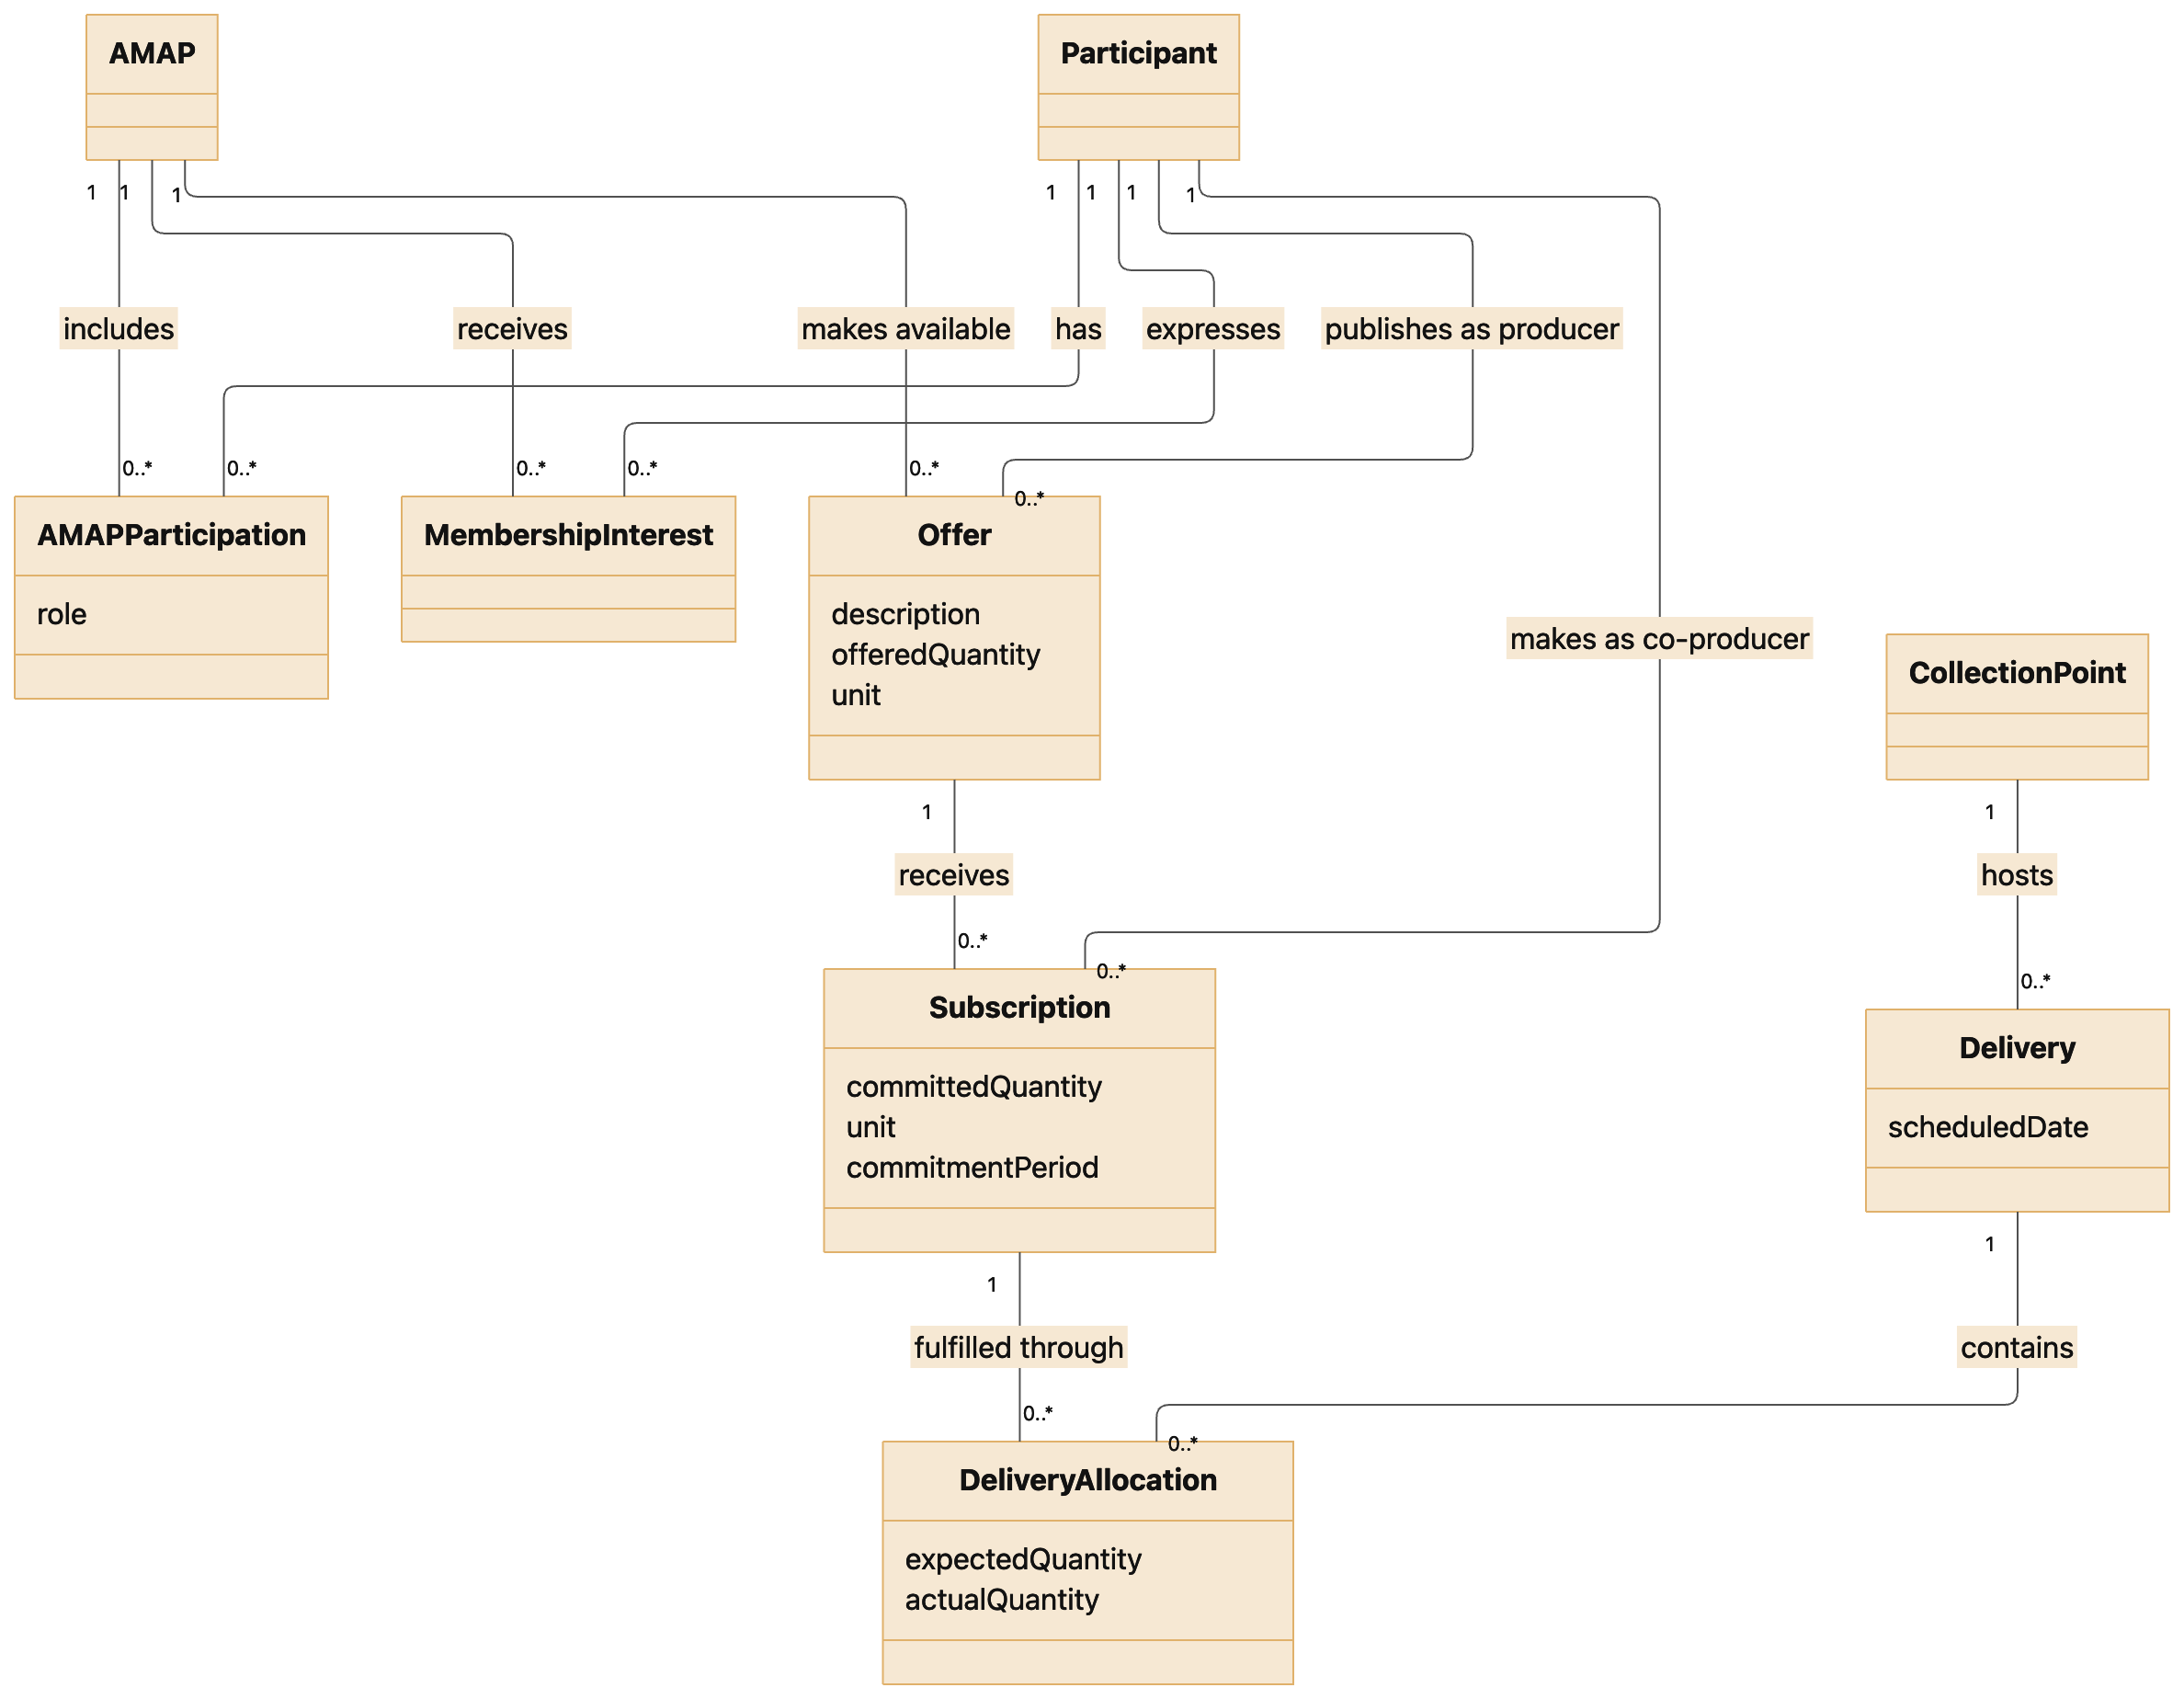
\includegraphics[width=0.82\linewidth]{figures/domain-model.png}
\caption{Core domain model. Sources and modelling choices are described in the relationship table below.}\label{fig:domain-model}
\end{figure}
{\footnotesize
\begin{longtable}{>{\raggedright\arraybackslash\hspace{0pt}}p{\dimexpr 0.176\linewidth-2\tabcolsep\relax}>{\raggedright\arraybackslash\hspace{0pt}}p{\dimexpr 0.412\linewidth-2\tabcolsep\relax}>{\raggedright\arraybackslash\hspace{0pt}}p{\dimexpr 0.412\linewidth-2\tabcolsep\relax}}
\caption{Relationships of the core domain model}\\
\rowcolor{hdr}\textcolor{white}{\textbf{Relationship}} & \textcolor{white}{\textbf{Meaning}} & \textcolor{white}{\textbf{Basis}} \\ \endfirsthead
\rowcolor{hdr}\textcolor{white}{\textbf{Relationship}} & \textcolor{white}{\textbf{Meaning}} & \textcolor{white}{\textbf{Basis}} \\ \endhead
AMAP and its members & An AMAP can have several producers and co-producers. People can participate in more than one AMAP. & S1-Q1; IN-P; S2-C4, S2-F. \\ \hline
Producer and offer & Each offer identifies the producer responsible for it. A producer can publish several offers, such as a basket and additional products. & S1-Q2; IN-P. \\ \hline
Offer and subscription & A subscription records one co-producer's commitment to one offer. Several co-producers can subscribe to the same offer. A co-producer can have subscriptions with different producers. & S1-Q2, S1-Q5; IN-C. Representing each offer commitment separately is the modelling choice introduced in Section 4. \\ \hline
Subscription and delivery & A subscription can cover several deliveries. A delivery can serve several subscriptions. Each delivery allocation records what is expected and what is actually delivered for one subscription. & S1-Q2, S1-Q4; S1-Q7. The allocation is a proposed way to represent this relationship. \\ \hline
Delivery and collection point & An AMAP may offer several collection points. Each scheduled delivery identifies its collection point, which can be used again on other dates. & S1-Q4; S2-F. Reusing a collection-point record is a modelling choice. \\ \hline
\end{longtable}}
For example, commitments to one producer's basket and another producer's eggs remain separate subscriptions, even when collected together. [S1-Q2, S1-Q4; IN-C]


\subsection{Community and membership}

Membership links a person to an AMAP; a subscription links them to a specific offer. Joining a community does not itself place an order. [S1-Q1 to S1-Q2, S1-Q5; modelling distinction]

People can browse nearby AMAPs, products and subscription options before joining, and may join several communities. A waiting list records interest when no places are available. The producer role alone does not confer admission authority (FR-11). [S1-Q5; S2-P4, S2-C4, S2-F]

AMAP management sets the delivery calendar and approves pauses and cancellations. Unsuitable dates can be discussed internally. [S2-P3 to S2-P4, S2-C3]

Each AMAP chooses payments through amaply or externally and may offer several collection points. Remaining membership and permission decisions are listed in Section 4.2. [S2-P1, S2-F]


\subsection{Offers and commitments}

An offer describes a basket or individual product; a subscription records the agreed quantity and period. The co-producer favours seasonal vegetable baskets, with items such as eggs, milk and bread selected individually. [S1-Q2, S1-Q5; S2-C2]

The commitment period says how long the agreement lasts; the schedule says when deliveries occur. A several-month commitment may, for example, have fortnightly deliveries. [S1-Q2, S1-Q4; IN-P]

Food preferences guide the producer without guaranteeing substitutions or allergy management. [S1-Q6; IN-C]

Producers need funds before delivery. The co-producer prefers one payment across AMAPs, distributed by the AMAP, without paying the whole season at once. Combined payment and distribution remain preferences; recipient and invoicing arrangements are unresolved. [S2-P1, S2-C1]

A pause or cancellation changes the commitment only after AMAP management approval. A combined payment does not merge subscriptions. Other change rules remain open (Section 4.2). [S2-P3, S2-C3; modelling distinctions]

\begin{figure}[htbp]\centering
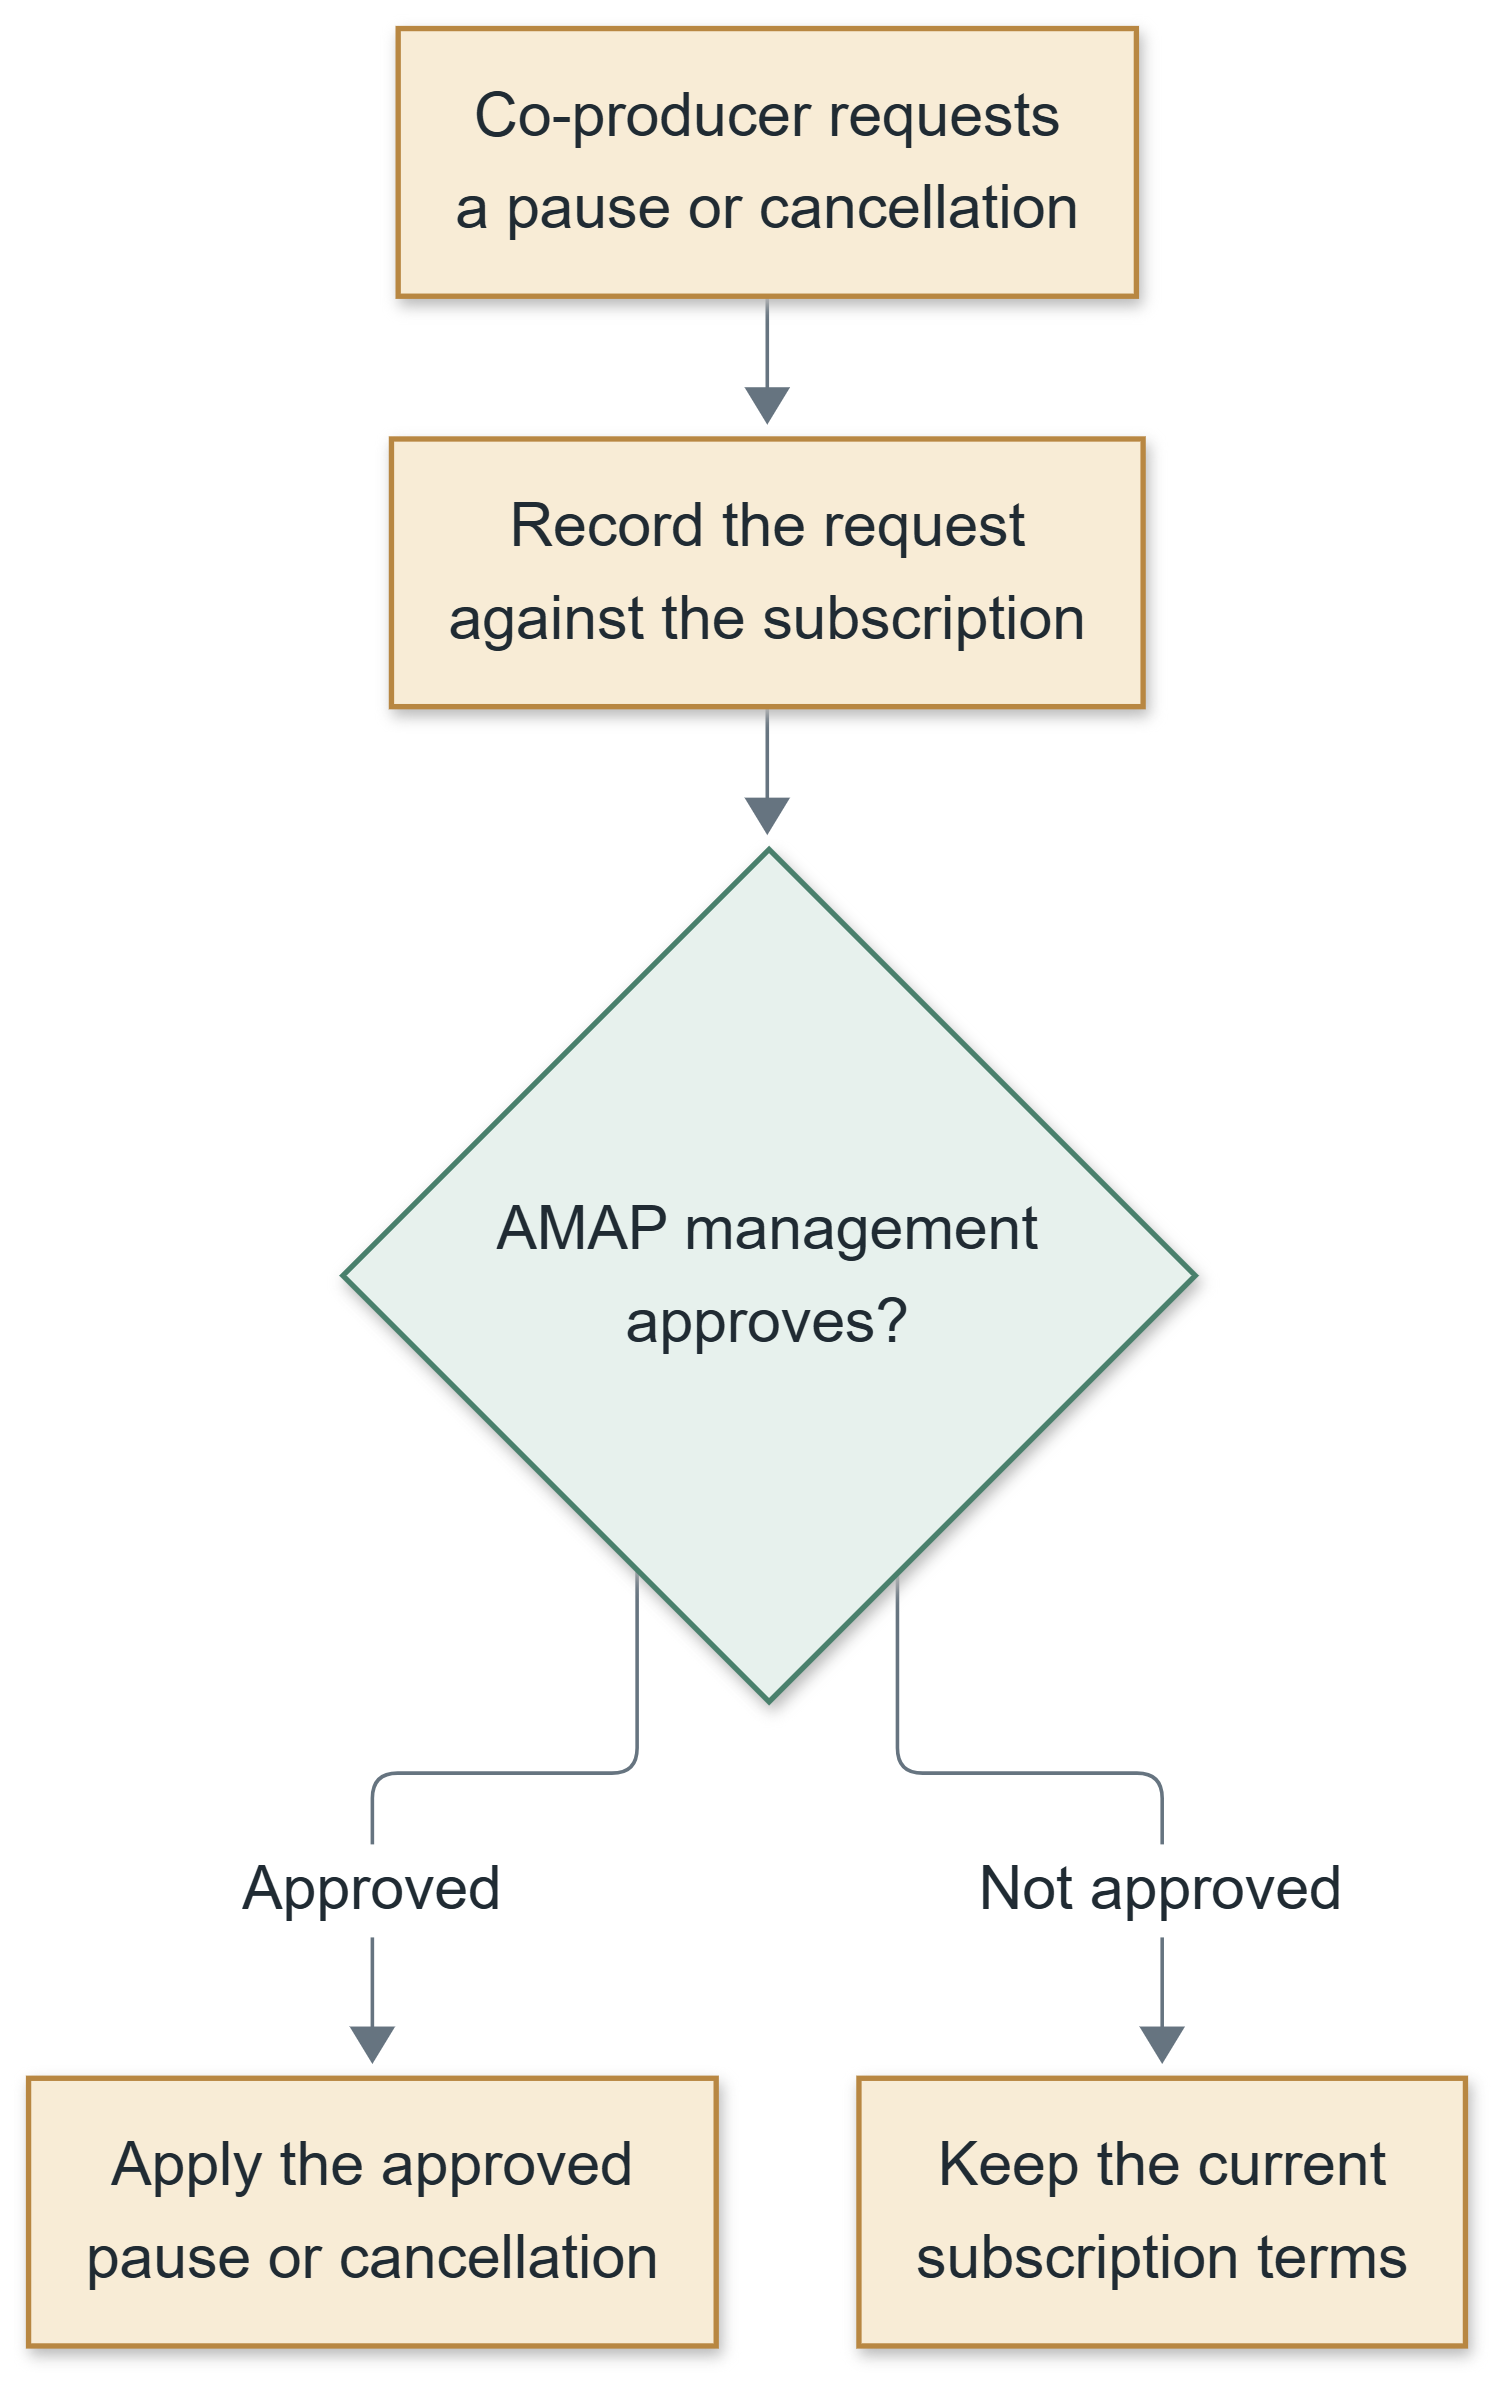
\includegraphics[width=0.39\linewidth]{figures/subscription-change.png}
\caption{Pause and cancellation approval. [S2-P3, S2-C3; request records and process layout are proposed. Dates and financial effects remain open.]}\label{fig:subscription-change}
\end{figure}

\subsection{Deliveries and communication}

A delivery links subscriptions to a date and collection point. Allocations record expected and delivered quantities. Collection confirmation is an optional proposal, separate from delivery recording; managing baskets left uncollected is not required. [S1-Q7; IN-P; IN-C; S2-P4 to S2-P5]

The producer chooses how to resolve a missing delivery, as shown below. Credit-use and seasonal-balance rules remain open (Section 4.2). [S2-P2]

\begin{figure}[htbp]\centering
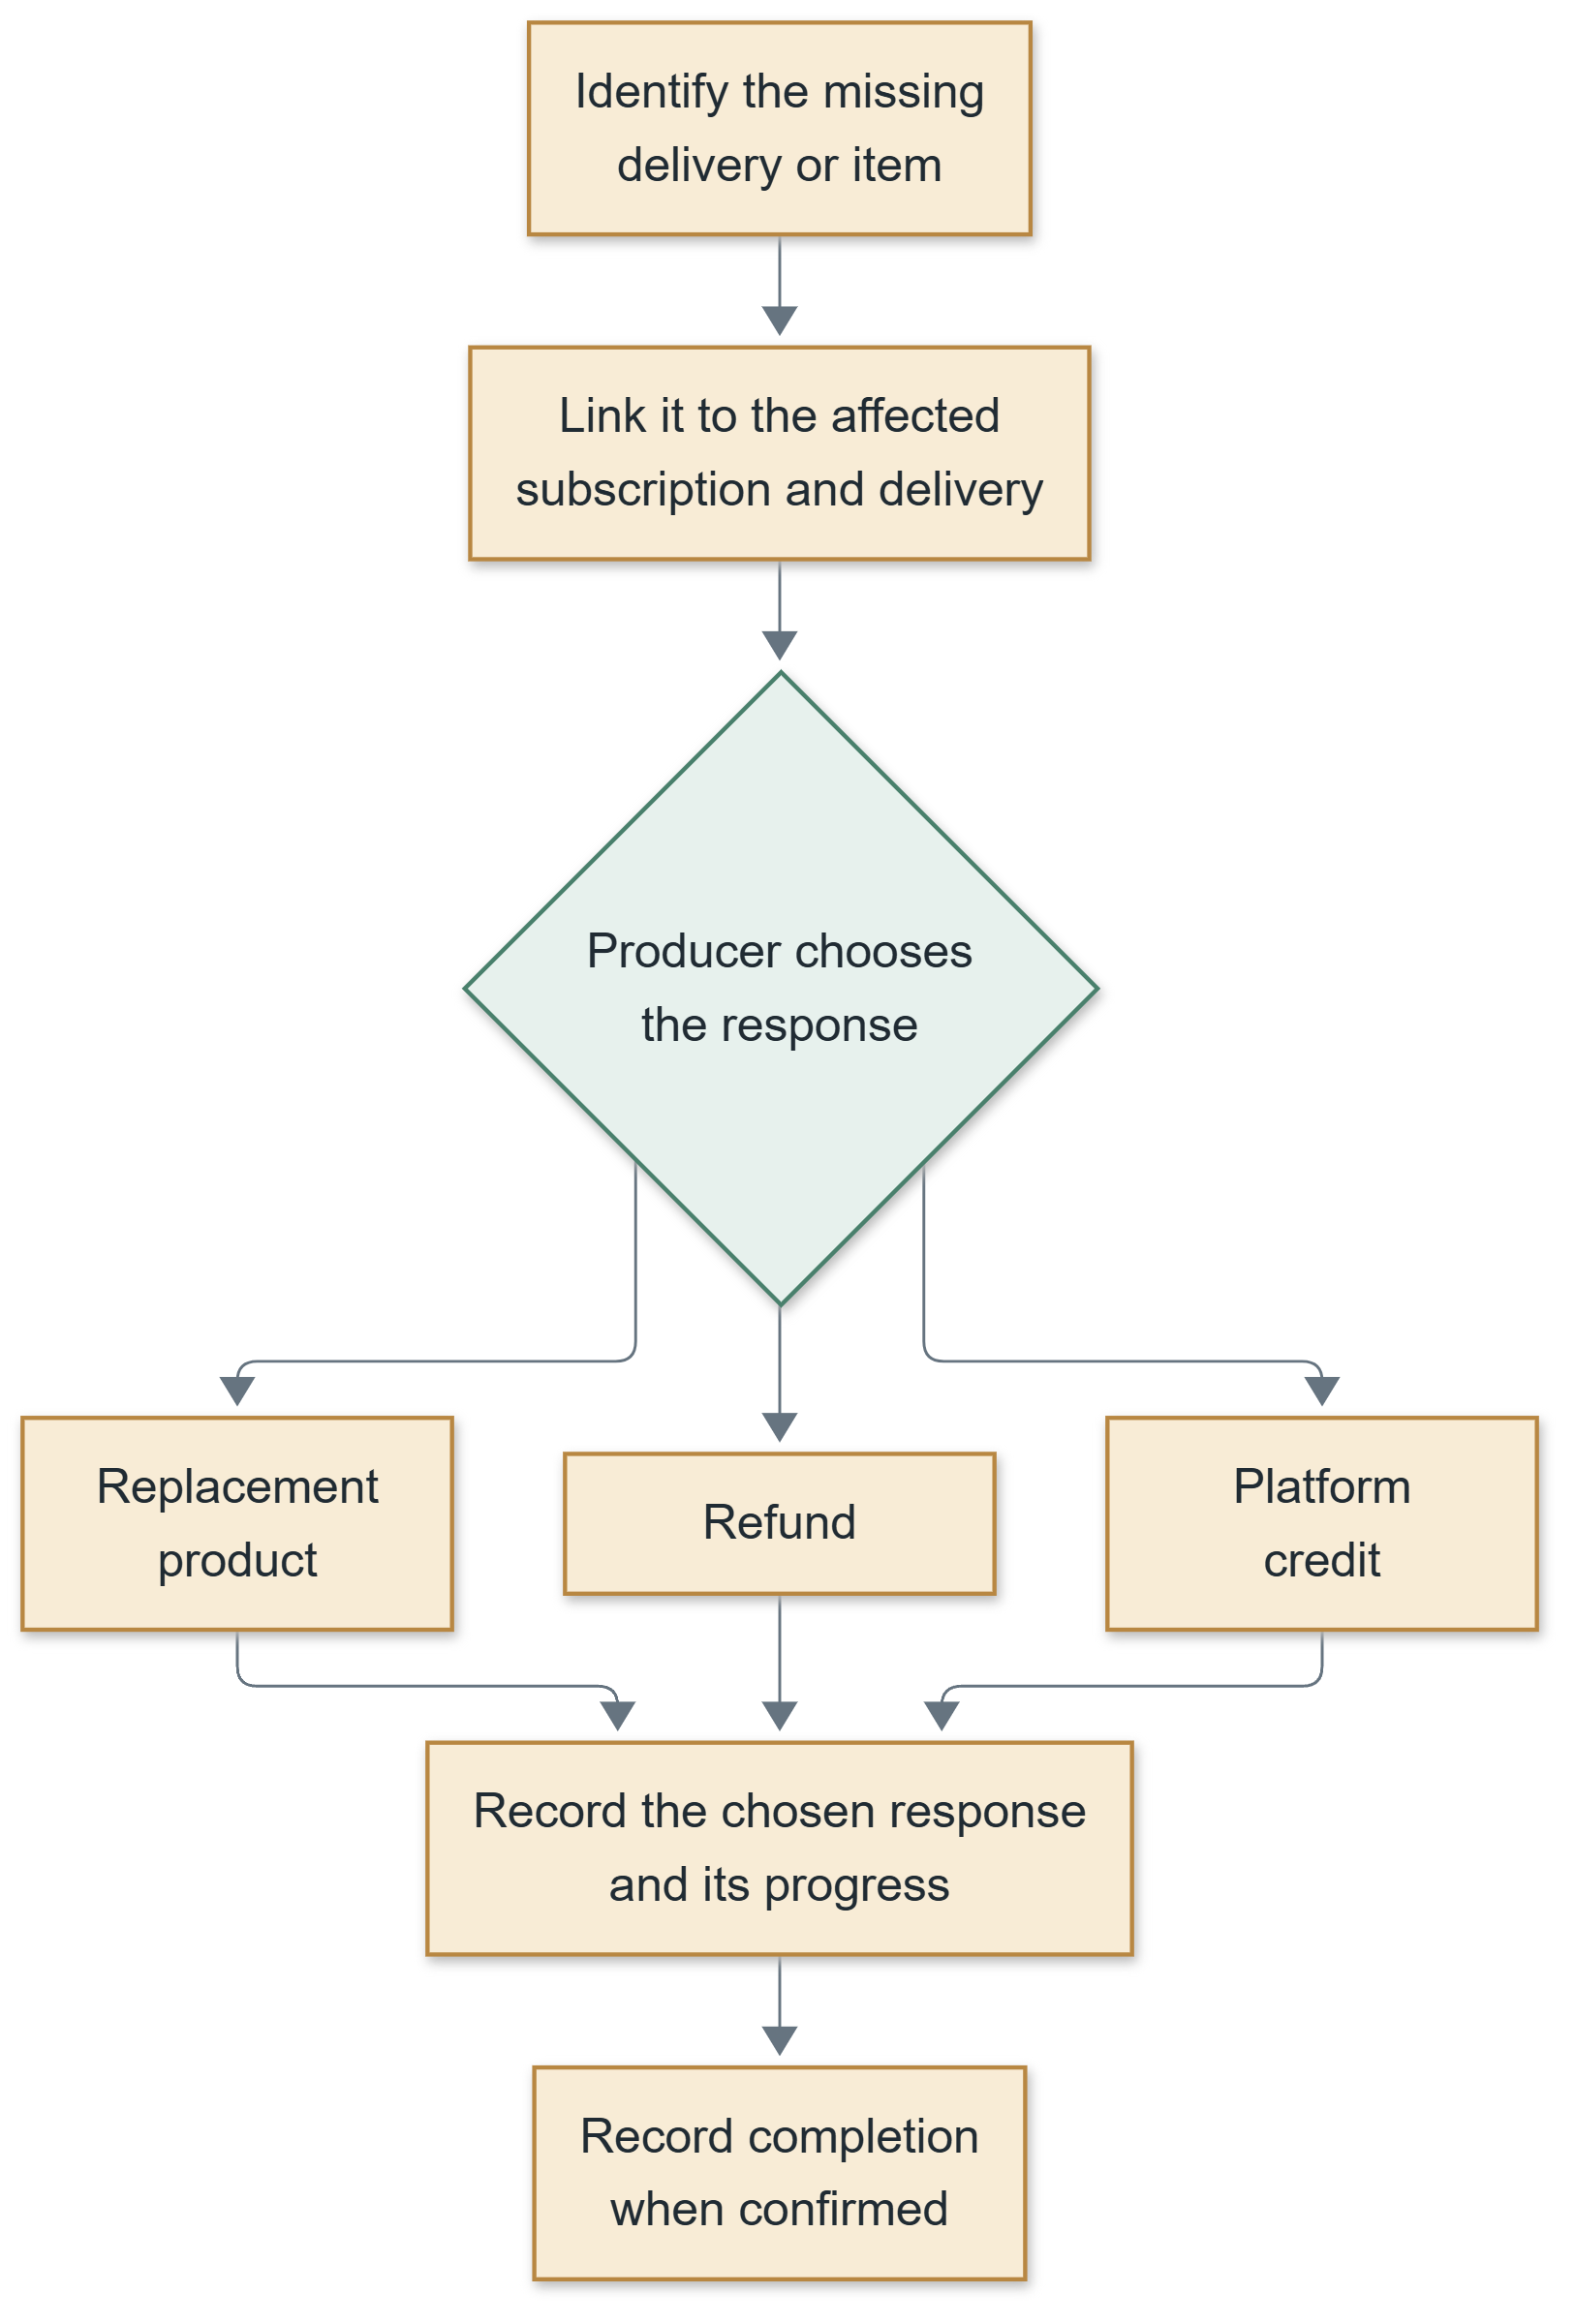
\includegraphics[width=0.39\linewidth]{figures/missing-delivery.png}
\caption{Missing-delivery response. [S2-P2; record links and progress tracking are proposed.]}\label{fig:missing-delivery}
\end{figure}
Communication includes collection notices, farm news, producer reminders and requested in-platform chat. Informal discussion and help from AMAP management are preferred to a formal dispute process. Reminder timing and chat details are covered in Section 6. [S1-Q4; S1-Q7; S2-P5, S2-C3]

A co-producer reporting an absence is prompted to choose another collector, an institution or other co-producers receiving the food. Pickup identity verification is not required by default; an AMAP may choose it. [S2-P5]


\subsection{Season and distribution view}

This view, written by Rodrigo Monteiro, models the same domain from the season and distribution day, using the words of the desk research [MR]. It is conceptual and its attributes are examples. A multiplicity next to an entity says how many instances of that entity relate to one instance of the other; a filled diamond marks composition, where the parts do not exist without the whole.

A farm, run by producers, offers a season. A co-producer subscribes to a season, choosing a share type and a pickup point, and pays in instalments. For each pickup date the producer creates a distribution, and every subscription gets a basket in it. If the co-producer will be away, an absence is recorded against the basket. A crop loss or missing product is recorded as a shortage, linked to the distributions it affects.

\begin{figure}[htbp]\centering
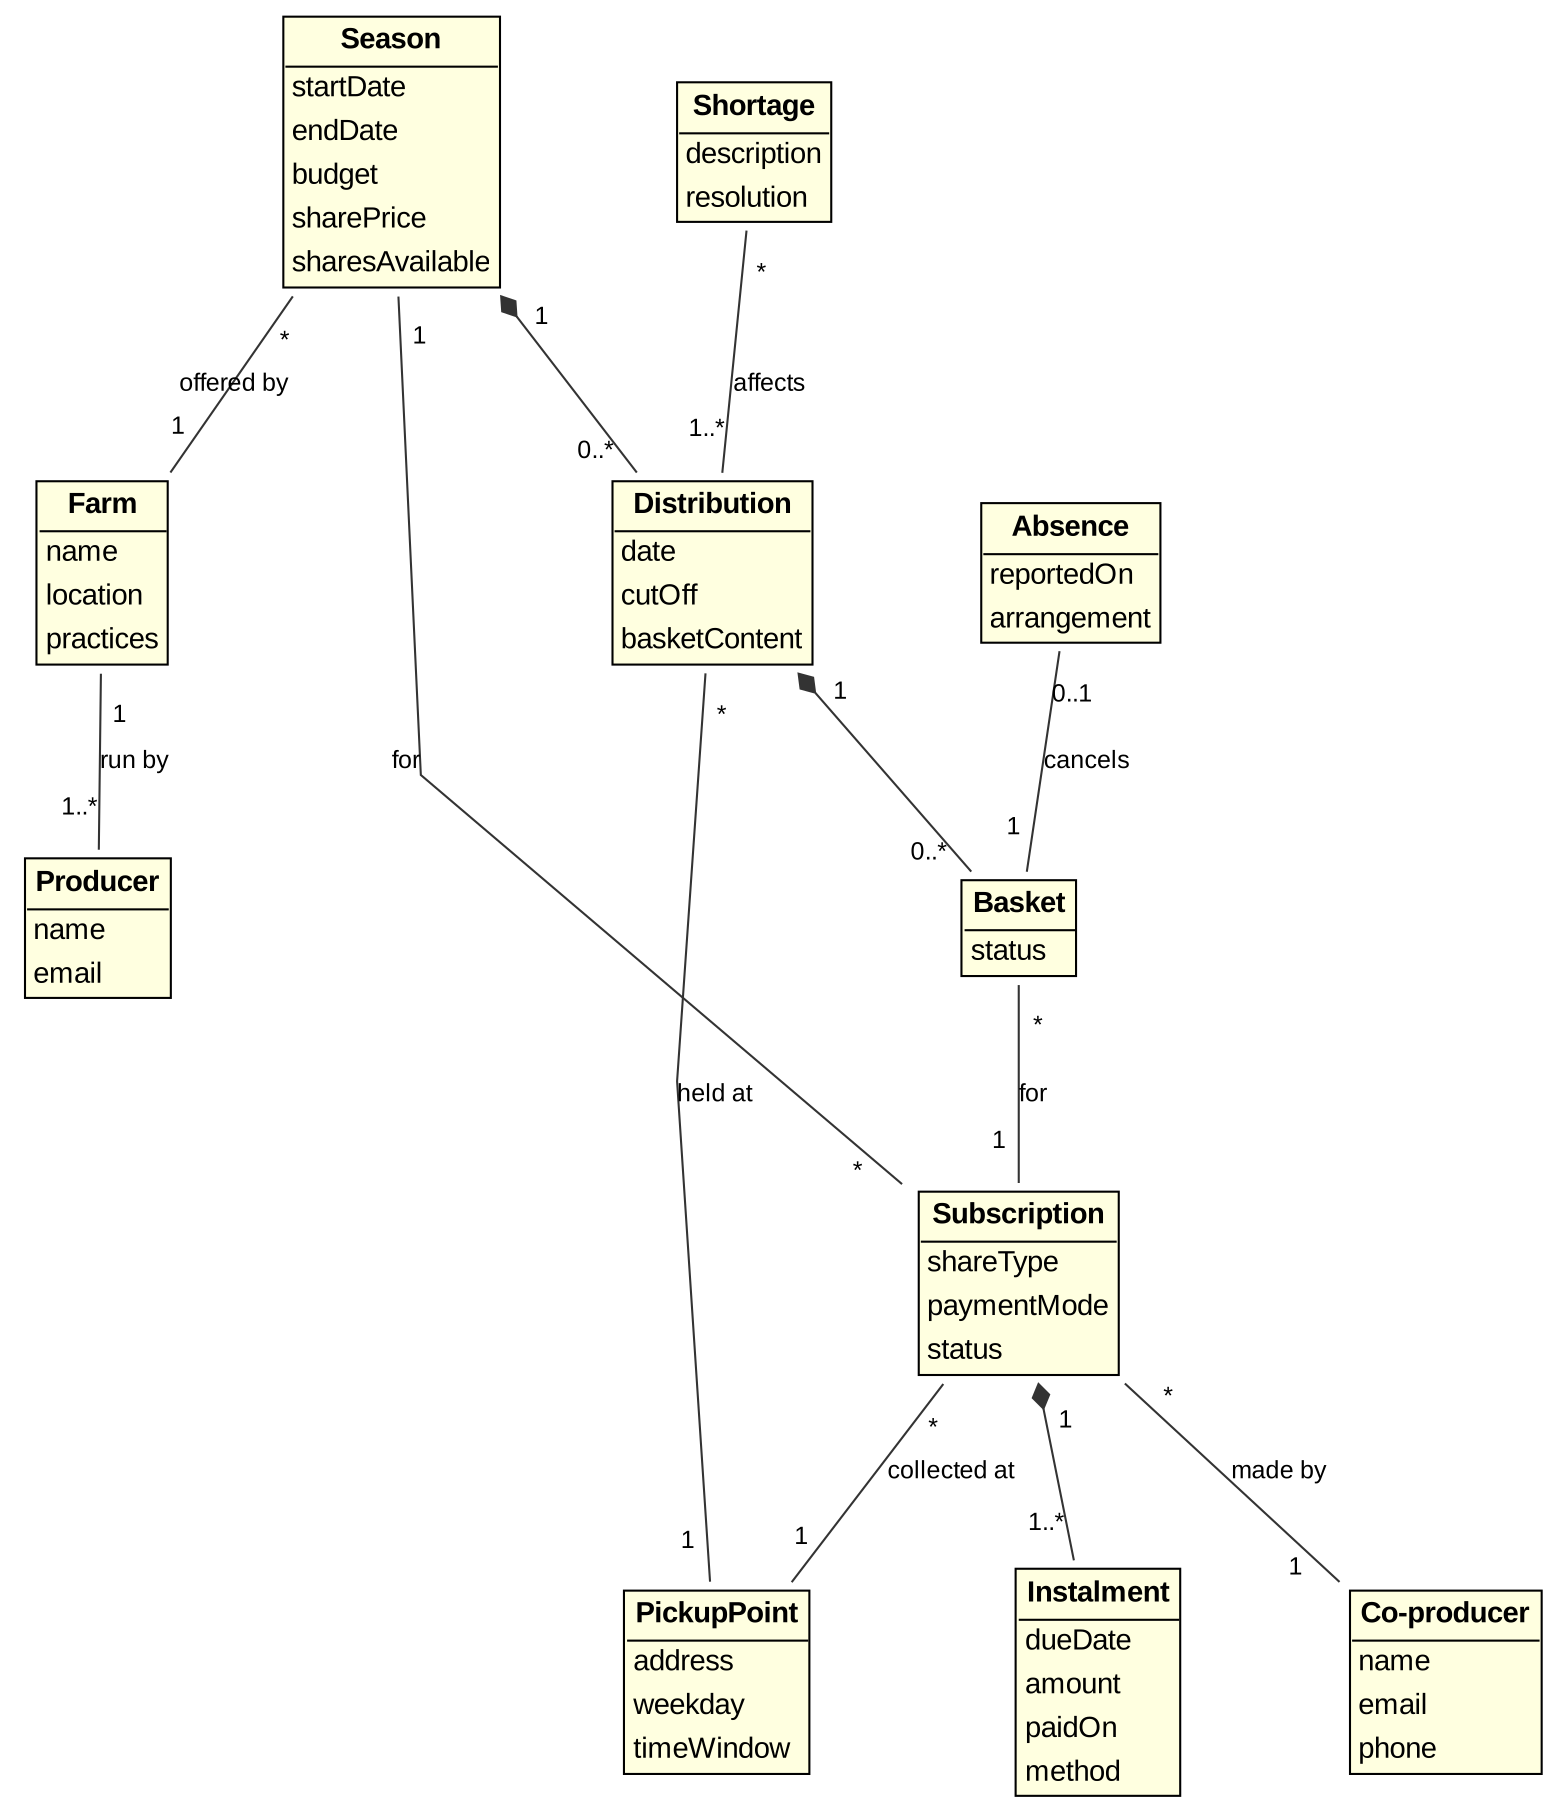
\includegraphics[width=0.64\linewidth]{figures/rodrigo-domain-model.png}
\caption{Season and distribution domain model (R. Monteiro)}\label{fig:rodrigo-domain-model}
\end{figure}
The entities are grouped in three bounded contexts. The same word can mean different things in each: a subscription is a contract in seasons and payments, and in distribution it is only the reason a basket exists. The season report and the impact indicators are calculated from this data and are not entities.


\subsubsection{People and places}

{\footnotesize
\begin{longtable}{>{\raggedright\arraybackslash\hspace{0pt}}p{\dimexpr 0.212\linewidth-2\tabcolsep\relax}>{\raggedright\arraybackslash\hspace{0pt}}p{\dimexpr 0.788\linewidth-2\tabcolsep\relax}}
\caption{Entities: people and places}\\
\rowcolor{hdr}\textcolor{white}{\textbf{Entity}} & \textcolor{white}{\textbf{Description}} \\ \endfirsthead
\rowcolor{hdr}\textcolor{white}{\textbf{Entity}} & \textcolor{white}{\textbf{Description}} \\ \endhead
Producer & Works on a farm and runs its seasons. \\ \hline
Co-producer & Pays for a share. \\ \hline
Farm & The place of production, with its location and practices. Run by one or more producers. \\ \hline
PickupPoint & The place where one group of co-producers collects baskets, on a weekday and in a time window. \\ \hline
\end{longtable}}

\subsubsection{Seasons and payments}

{\footnotesize
\begin{longtable}{>{\raggedright\arraybackslash\hspace{0pt}}p{\dimexpr 0.212\linewidth-2\tabcolsep\relax}>{\raggedright\arraybackslash\hspace{0pt}}p{\dimexpr 0.788\linewidth-2\tabcolsep\relax}}
\caption{Entities: seasons and payments}\\
\rowcolor{hdr}\textcolor{white}{\textbf{Entity}} & \textcolor{white}{\textbf{Description}} \\ \endfirsthead
\rowcolor{hdr}\textcolor{white}{\textbf{Entity}} & \textcolor{white}{\textbf{Description}} \\ \endhead
Season & A period of production and distribution, for example 24 weeks, with a budget, a share price and a number of shares. Offered by one farm. \\ \hline
Subscription & A co-producer's commitment to a season: one share (full or half), one pickup point, paid in full or by instalments. \\ \hline
Instalment & A scheduled amount with a due date. Records when and how it was paid. \\ \hline
\end{longtable}}
The instalments of a subscription add up to the price of the share. A season does not accept more subscriptions than shares available.


\subsubsection{Baskets and distribution}

{\footnotesize
\begin{longtable}{>{\raggedright\arraybackslash\hspace{0pt}}p{\dimexpr 0.212\linewidth-2\tabcolsep\relax}>{\raggedright\arraybackslash\hspace{0pt}}p{\dimexpr 0.788\linewidth-2\tabcolsep\relax}}
\caption{Entities: baskets and distribution}\\
\rowcolor{hdr}\textcolor{white}{\textbf{Entity}} & \textcolor{white}{\textbf{Description}} \\ \endfirsthead
\rowcolor{hdr}\textcolor{white}{\textbf{Entity}} & \textcolor{white}{\textbf{Description}} \\ \endhead
Distribution & One handing-out of baskets, at a pickup point on a date, with a cut-off for absences and the content of the basket. \\ \hline
Basket & What one subscription receives in one distribution. Its status is planned, collected, unclaimed or passed on to someone else. \\ \hline
Absence & A co-producer's notice that a basket will not be collected, with who receives it instead: a named person, an institution or other co-producers. \\ \hline
Shortage & A recorded crop loss or missing product, with a description and the resolution the producer chose: replacement, refund or credit. \\ \hline
\end{longtable}}
An absence has to be recorded before the cut-off of the distribution, and the co-producer says who receives the basket (FR-32). A basket nobody collects is only recorded as unclaimed (FR-34). The producer chooses how a shortage is resolved (FR-36). The cut-off is a proposal that has to be checked with real groups (AS-13).


\subsubsection{Relation to the core model}

The two views describe the same domain at different levels and must be reconciled during validation:

\begin{itemize}
  \item \textbf{Equivalent concepts.} PickupPoint corresponds to CollectionPoint, Distribution to Delivery, and Basket to DeliveryAllocation (what one subscription receives on one date). Producer and Co-producer correspond to Participant with a role in an AMAP participation.
  \item \textbf{Different centre.} The core model is organised around the AMAP and its offers, as described in the interviews [S1-Q2, S2-F]; this view is organised around the farm and its season, with the share as the unit of commitment. A season with shares can be read as an offer of type seasonal basket (FR-20).
  \item \textbf{Concepts only in this view.} Farm, Instalment, Absence and Shortage. Instalment, absence and shortage are covered by FR-43, FR-32 and FR-35 to FR-36.
  \item \textbf{Rule to confirm.} The cut-off for absences is not in the interview evidence; see AS-13.
\end{itemize}

\section{External interface requirements}

This section defines the views and exchanges needed for users, external services and devices.

Sources use the codes of Table 1. Workflows follow the session notes and S2. Payment processing uses an external licensed provider under CO-2 and invoicing uses certified software under FR-49. These are integration requirements in this draft; no specific providers have been selected. Technical details remain undecided. Analysis proposals are labelled.


\subsection{User interfaces}

The following views group related information and actions. Each shall identify the relevant producer and AMAP. [S1-Q1 to S1-Q2; IN-P; grouping into views is proposed]

{\footnotesize
\begin{longtable}{>{\raggedright\arraybackslash\hspace{0pt}}p{\dimexpr 0.087\linewidth-2\tabcolsep\relax}>{\raggedright\arraybackslash\hspace{0pt}}p{\dimexpr 0.280\linewidth-2\tabcolsep\relax}>{\raggedright\arraybackslash\hspace{0pt}}p{\dimexpr 0.316\linewidth-2\tabcolsep\relax}>{\raggedright\arraybackslash\hspace{0pt}}p{\dimexpr 0.316\linewidth-2\tabcolsep\relax}}
\caption{User interface views}\\
\rowcolor{hdr}\textcolor{white}{\textbf{ID}} & \textcolor{white}{\textbf{View and user}} & \textcolor{white}{\textbf{Information and actions}} & \textcolor{white}{\textbf{Source or reasoning}} \\ \endfirsthead
\rowcolor{hdr}\textcolor{white}{\textbf{ID}} & \textcolor{white}{\textbf{View and user}} & \textcolor{white}{\textbf{Information and actions}} & \textcolor{white}{\textbf{Source or reasoning}} \\ \endhead
UI-01 & AMAP discovery, for a person looking for a community & Browse AMAPs geographically and view their collection points, products and subscription options before joining. Express interest in joining or register interest on a waiting list when there are no places. & S1-Q5; S2-C4, S2-F. Coordinator approval follows FR-11; detailed admission steps and waiting-list priority remain open. \\ \hline
UI-02 & Offers and subscriptions, for a co-producer & Show the producer, basket or individual product, quantity, unit, commitment period and delivery schedule. Support seasonal baskets alongside individually selected products. Let the person review the commitment before submitting it. & S1-Q2, S1-Q5; S2-C2. Review before submission is proposed. \\ \hline
UI-03 & Personal subscription summary, for a co-producer & Show subscriptions across their AMAPs, producers, quantities, commitment periods, collection dates and locations. Distinguish a requested pause or cancellation from an approved change. & S2-P3, S2-C3 to S2-C4, S2-F; S1-Q2, S1-Q4. See REP-01. \\ \hline
UI-04 & Offer and delivery preparation, for a producer & Allow the producer to describe offers and quantities, view commitments to their offers, and see what to prepare for a selected delivery and AMAP. & S1-Q2; IN-P. The preparation summary is proposed in REP-02. \\ \hline
UI-05 & Producer presentation, for producers and people viewing their information & Allow a producer to add certificates, photographs or descriptions of production practices and make the agreed information available to its intended audience. & S1-Q9. File limits and visibility rules remain open. \\ \hline
UI-06 & Delivery information and community news, for producers and co-producers & Show collection details, farm news, harvest changes and relevant notices. Provide producers with delivery reminders. & S1-Q1, S1-Q4; S1-Q7; S2-P5. One day before delivery is an example; exact timing and channels remain open. \\ \hline
UI-07 & Amounts and payment options, for a co-producer & Show amounts by producer and AMAP, currency, payment route, refunds and credit. Support the AMAP's payment choice. Combined payment across AMAPs without full-season prepayment is a preference to investigate. & S2-P1 to S2-P2, S2-C1; REP-03. \\ \hline
UI-08 & Advance absence arrangements, for a co-producer & Prompt an absent person to choose another collector, an institution or other co-producers receiving the food. Collection confirmation is optional; managing uncollected baskets is not required. & S2-P5. Pickup verification is optional; deadlines and contact fields remain open. \\ \hline
UI-09 & Calendar and subscription decisions, for AMAP management & Set the delivery calendar and approve or reject pause/cancellation requests. Distinguish submission from approval. & S2-P3 to S2-P4, S2-C3; approval display is proposed. \\ \hline
UI-10 & Missing-delivery resolution, for a producer & Select replacement, refund or credit for the affected item or delivery. Show the co-producer the response and recorded progress. & S2-P2; progress display is proposed. \\ \hline
UI-11 & In-platform chat, for direct discussion & Support informal discussion and help from AMAP management. & Requested in S2-C3; detailed access and retention rules remain open. \\ \hline
\end{longtable}}
The following presentation rules are proposed for clarity and consistency. [S1-Q1, S1-Q6; IN-C]

{\footnotesize
\begin{longtable}{>{\raggedright\arraybackslash\hspace{0pt}}p{\dimexpr 0.121\linewidth-2\tabcolsep\relax}>{\raggedright\arraybackslash\hspace{0pt}}p{\dimexpr 0.440\linewidth-2\tabcolsep\relax}>{\raggedright\arraybackslash\hspace{0pt}}p{\dimexpr 0.440\linewidth-2\tabcolsep\relax}}
\caption{Presentation rules}\\
\rowcolor{hdr}\textcolor{white}{\textbf{ID}} & \textcolor{white}{\textbf{Proposed presentation rule}} & \textcolor{white}{\textbf{Reason}} \\ \endfirsthead
\rowcolor{hdr}\textcolor{white}{\textbf{ID}} & \textcolor{white}{\textbf{Proposed presentation rule}} & \textcolor{white}{\textbf{Reason}} \\ \endhead
UI-12 & Use the same terms throughout the interface, including producer, co-producer, offer, subscription and delivery. & Keeps the interface consistent with the domain model in Section 5. \\ \hline
UI-13 & Show quantity units beside quantities and currencies beside amounts. Explain how often a price applies when that basis is known. & Helps people distinguish a monthly amount, a price per product and a delivery quantity. \\ \hline
UI-14 & After a submission, say whether it was saved. If a field needs correction, identify it and explain what the user should change. & Prevents uncertainty about whether an offer or commitment was recorded. \\ \hline
UI-15 & Present expected quantities and actual delivery quantities with different labels. & Makes seasonal variation visible without confusing the agreement with the delivery record; see DR-03. \\ \hline
\end{longtable}}
Layouts, accessibility targets, screen sizes, browser support and the complete permission model need validation. A web interface for phones and computers is proposed; a native application is undecided.


\subsection{Software interfaces}

The following service interfaces are candidates for supporting the agreed workflows. Specific providers and versions remain undecided; payment and invoicing integrations follow CO-2 and FR-49, while the other external services remain candidates. [OQ; S2-P1, S2-P5, S2-C3 to S2-C4, S2-F]

\begin{figure}[htbp]\centering
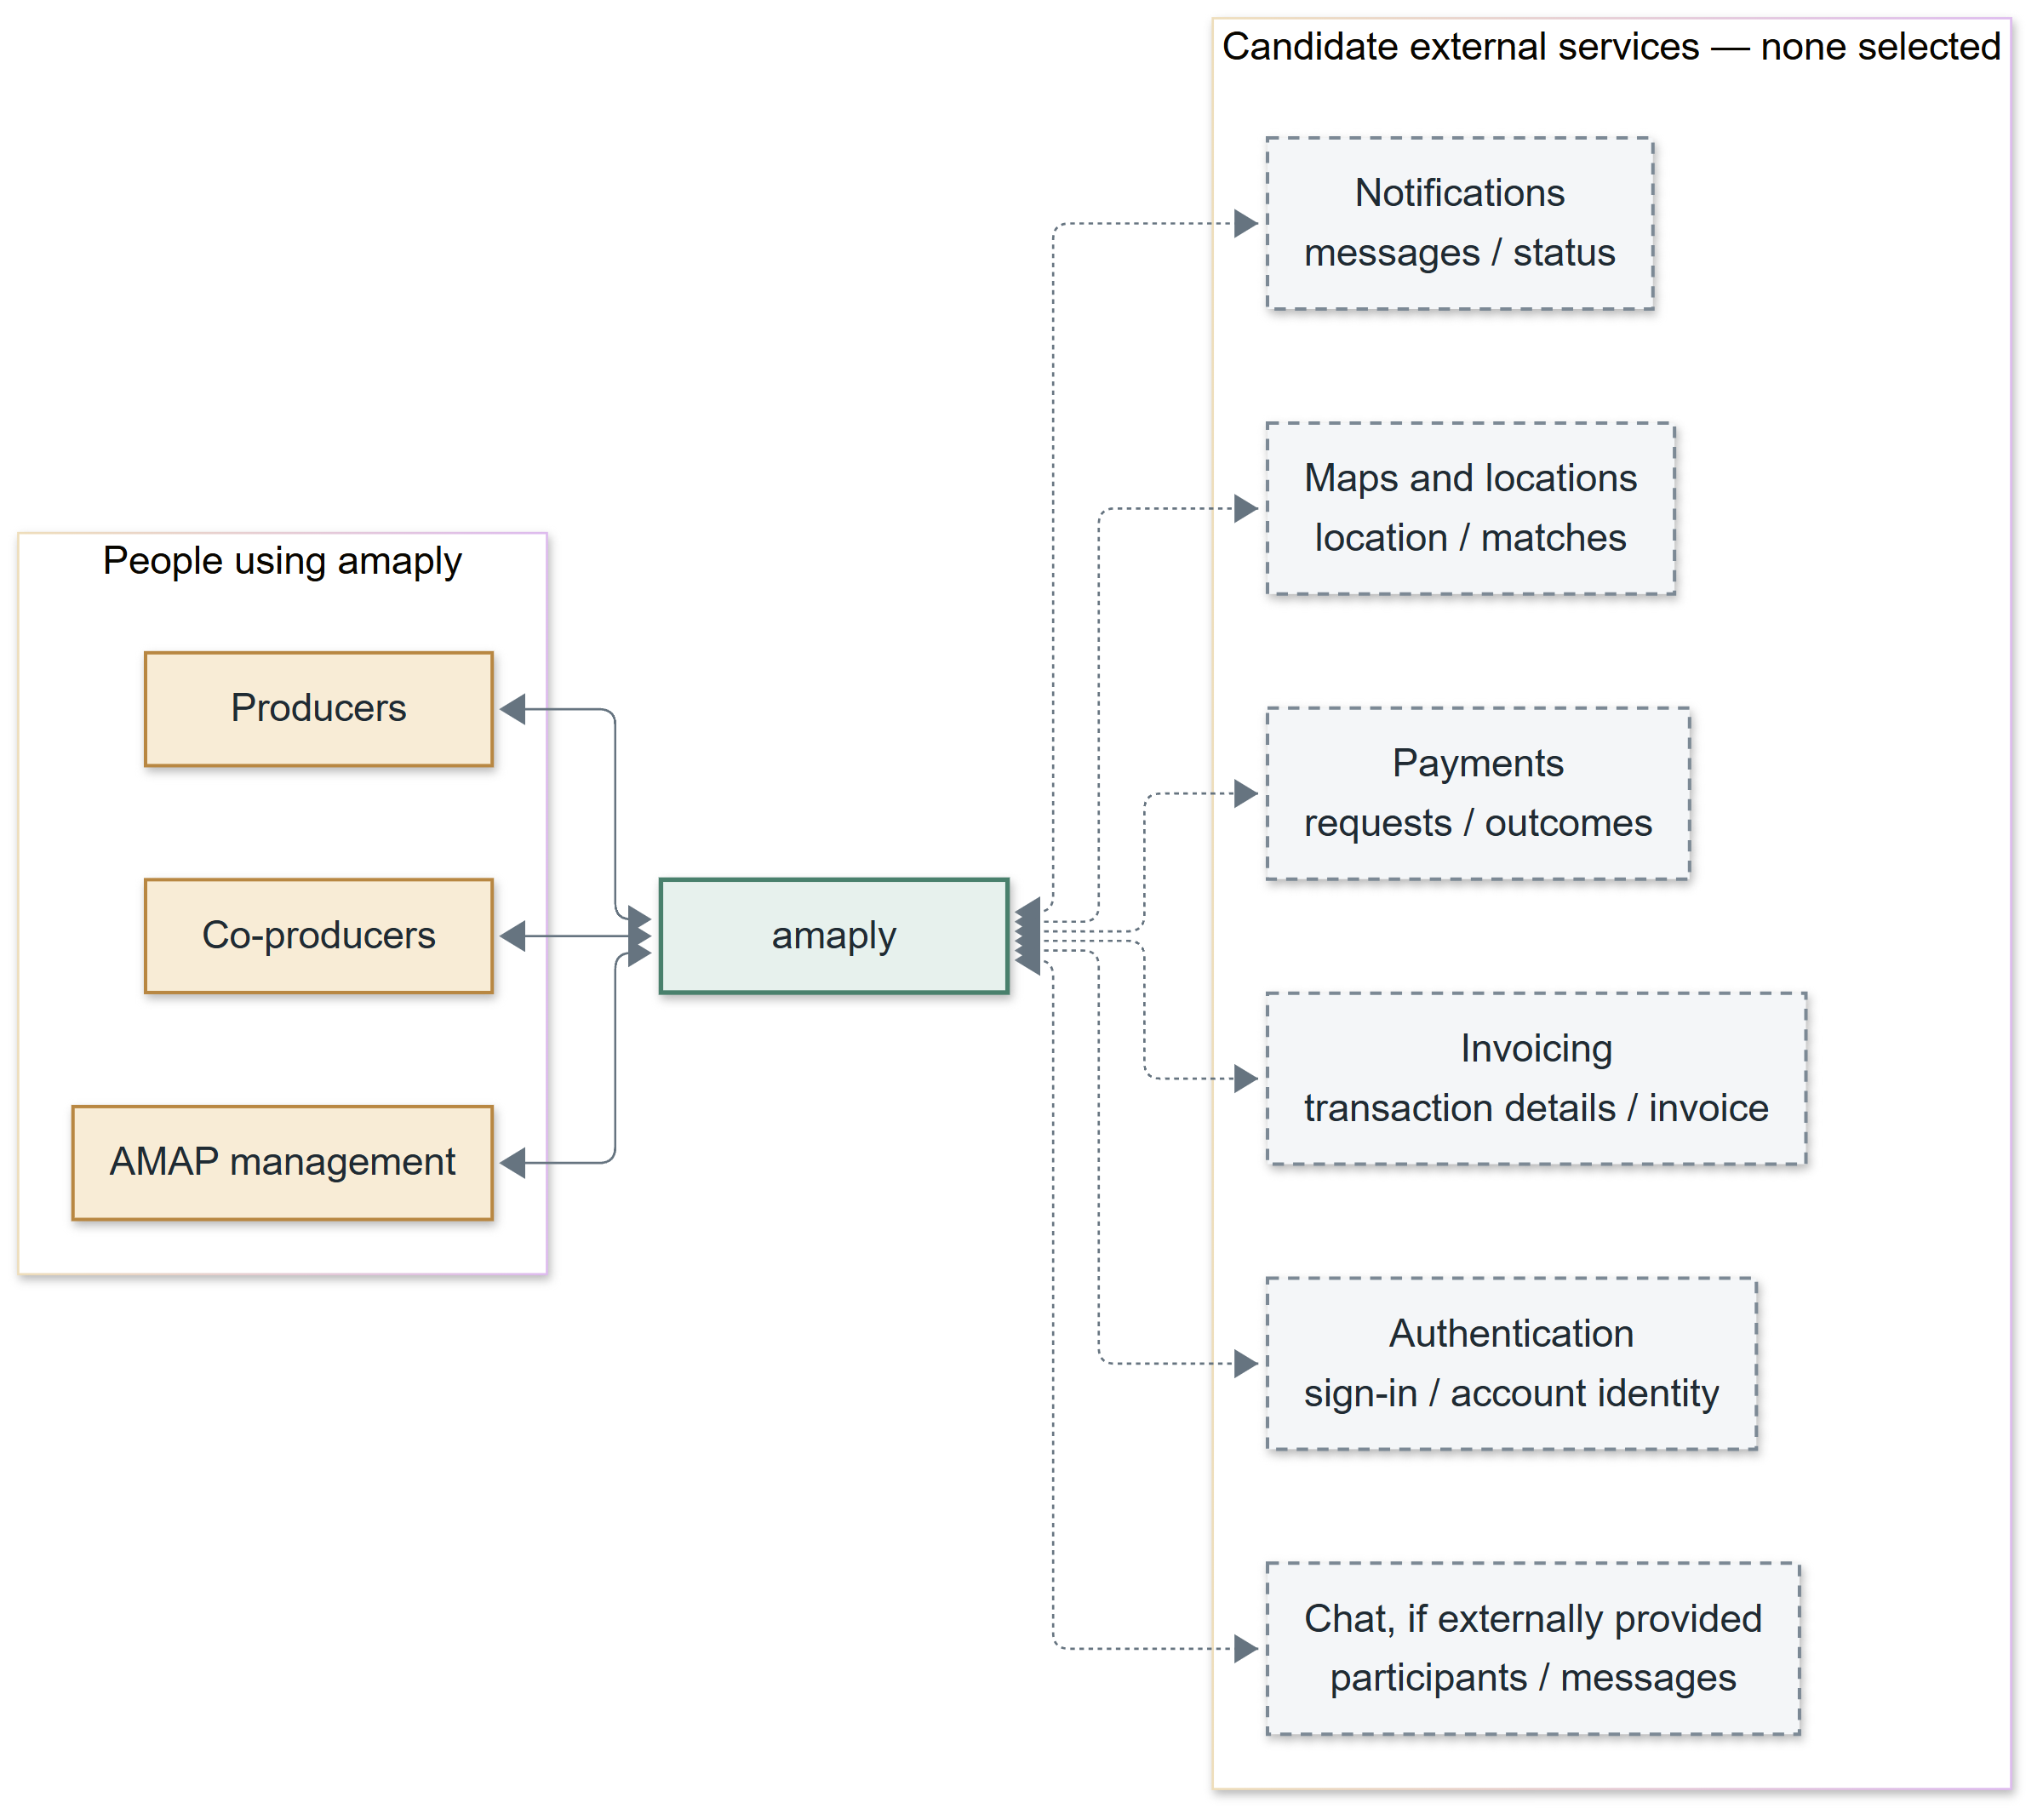
\includegraphics[width=0.61\linewidth]{figures/external-interfaces.png}
\caption{Interface overview. Solid lines show user interaction; dashed lines show candidate integrations. No providers are selected. [OQ; S2-P1, S2-P5, S2-C3 to S2-C4, S2-F; proposed interface layout.]}\label{fig:external-interfaces}
\end{figure}
{\footnotesize
\begin{longtable}{>{\raggedright\arraybackslash\hspace{0pt}}p{\dimexpr 0.183\linewidth-2\tabcolsep\relax}>{\raggedright\arraybackslash\hspace{0pt}}p{\dimexpr 0.409\linewidth-2\tabcolsep\relax}>{\raggedright\arraybackslash\hspace{0pt}}p{\dimexpr 0.409\linewidth-2\tabcolsep\relax}}
\caption{Candidate software interfaces}\\
\rowcolor{hdr}\textcolor{white}{\textbf{Candidate interface}} & \textcolor{white}{\textbf{Information sent and received if adopted}} & \textcolor{white}{\textbf{Purpose and open decisions}} \\ \endfirsthead
\rowcolor{hdr}\textcolor{white}{\textbf{Candidate interface}} & \textcolor{white}{\textbf{Information sent and received if adopted}} & \textcolor{white}{\textbf{Purpose and open decisions}} \\ \endhead
Notification service & Send the recipient address for the selected channel, message content and delivery or community reference; receive acceptance or failure information. & Notify co-producers about collection and remind producers before delivery. One day before delivery is an example; timing and channels remain to be agreed. [S1-Q4; S2-P5] \\ \hline
Location or mapping service & Send the location entered or selected by the user; receive matching places, coordinates or distances as needed. & Support geographic AMAP discovery and several collection locations per AMAP. Provider and device-location access remain undecided. [S2-C4, S2-F] \\ \hline
Payment service & Send a payment request with amount, currency, intended recipient and reference; receive its outcome. Exchanges for refunds, allocation or settlement must be defined if required by the selected payment arrangement. & Support AMAP-selected platform payments alongside external payments. Producers must be able to access funds before delivery. Combined payments are desired where feasible; recipient, fees, method list and reconciliation remain open. [S2-P1 to S2-P2, S2-C1] \\ \hline
Invoicing service & Exchange the seller, customer and transaction details required by an agreed invoicing process, and receive the invoice reference or document. & Support the certified invoicing integration specified in FR-49. No provider has been selected; the issuer depends on the AMAP legal setup and remains to be confirmed. [S1-Q10; OQ] \\ \hline
External authentication service & Exchange the information needed to establish a user session and identify the account, according to the selected sign-in method. & Support sign-in if an external identity provider is chosen. The provider, protocol and account-linking rules remain open. [OQ] \\ \hline
Optional chat service & If an external chat product is selected, exchange sender and recipient identifiers, message content and any agreed delivery information. & In-platform chat is requested, but using an external service is not a requirement. Permissions, retention, provider and protocol remain open. [S2-C3] \\ \hline
\end{longtable}}
Each selected integration needs a provider/version, message fields and format, authentication method and failure behaviour. The table gives preliminary exchanges.

MB Way and bank transfer are current methods; cash is not normally used. Apple Pay and PayPal were suggestions. The supported method list remains open. [S2-C1]


\subsection{Hardware interfaces}

No dedicated hardware interface is currently required. Phones and computers are proposed for portal access; supported devices and operating conditions remain undecided. [S1-Q4; S1-Q6; IN-P]

File uploads in UI-05 do not require direct camera or scanner control. Weighing scales, payment terminals and barcode readers have no specified integration. [S1-Q9]

Pickup verification is optional; any required verification device would need a separate interface specification. [S2-P5]


\subsection{Communication interfaces}

Communication channels and protocols remain to be selected. The following rules cover notifications, chat and service responses. [S1-Q1, S1-Q4; S1-Q7; S2-P5, S2-C3]

{\footnotesize
\begin{longtable}{>{\raggedright\arraybackslash\hspace{0pt}}p{\dimexpr 0.121\linewidth-2\tabcolsep\relax}>{\raggedright\arraybackslash\hspace{0pt}}p{\dimexpr 0.440\linewidth-2\tabcolsep\relax}>{\raggedright\arraybackslash\hspace{0pt}}p{\dimexpr 0.440\linewidth-2\tabcolsep\relax}}
\caption{Communication rules}\\
\rowcolor{hdr}\textcolor{white}{\textbf{ID}} & \textcolor{white}{\textbf{Requirement or proposed rule}} & \textcolor{white}{\textbf{Source or reasoning}} \\ \endfirsthead
\rowcolor{hdr}\textcolor{white}{\textbf{ID}} & \textcolor{white}{\textbf{Requirement or proposed rule}} & \textcolor{white}{\textbf{Source or reasoning}} \\ \endhead
COM-01 & Collection notifications shall identify the AMAP and collection location; date and time are proposed additions. Producers shall receive delivery reminders. & S1-Q4; S2-P5. One day before delivery is an example, not a fixed schedule. \\ \hline
COM-02 & Production news and explanations of harvest changes shall be available through the platform. The audience and any notification channel shall be agreed separately. & S1-Q7; audience and channel decisions remain open. \\ \hline
COM-03 & For the proposed web interface, use HTTPS for communication between the user's browser and amaply. & Proposed technical safeguard for the personal and financial information described in Section 4. Protocol configuration belongs to the later security specification. \\ \hline
COM-04 & If an external notification service is adopted, distinguish a message being accepted by that service from confirmed delivery to the recipient. A service failure shall not be shown as a successfully delivered notification. & Proposed rule to avoid giving users a misleading notification status. Delivery evidence depends on the selected service. \\ \hline
COM-05 & If a payment service is adopted, associate each received result with the payment request it concerns. Repeated delivery of the same result shall not create a second payment record. & Proposed rule to keep the amount summary consistent when an external service repeats a message. \\ \hline
COM-06 & Support in-platform chat and informal discussion with AMAP management. & Requested in S2-C3. Communication between separate AMAPs is unconfirmed. [S2-F] \\ \hline
\end{longtable}}
Remaining communication decisions: final reminder timing, channels, recipient rules, retries, message formats, chat access and retention, and response-time targets. Offline use and synchronisation are unconfirmed. Language rules are in Section 8. [S2-P5, S2-C3; analysis questions]


\section{Quality attributes}

This section specifies the other non-functional requirements. Each one is measurable so that it can be verified. Where values depend on open questions (mainly volumes), they are provisional and marked as such.


\subsection{Usability}

{\footnotesize
\begin{longtable}{>{\raggedright\arraybackslash\hspace{0pt}}p{\dimexpr 0.133\linewidth-2\tabcolsep\relax}>{\raggedright\arraybackslash\hspace{0pt}}p{\dimexpr 0.398\linewidth-2\tabcolsep\relax}>{\raggedright\arraybackslash\hspace{0pt}}p{\dimexpr 0.108\linewidth-2\tabcolsep\relax}>{\raggedright\arraybackslash\hspace{0pt}}p{\dimexpr 0.120\linewidth-2\tabcolsep\relax}>{\raggedright\arraybackslash\hspace{0pt}}p{\dimexpr 0.241\linewidth-2\tabcolsep\relax}}
\caption{Usability requirements}\\
\rowcolor{hdr}\textcolor{white}{\textbf{ID}} & \textcolor{white}{\textbf{Requirement}} & \textcolor{white}{\textbf{Prio.}} & \textcolor{white}{\textbf{Source}} & \textcolor{white}{\textbf{Justification}} \\ \endfirsthead
\rowcolor{hdr}\textcolor{white}{\textbf{ID}} & \textcolor{white}{\textbf{Requirement}} & \textcolor{white}{\textbf{Prio.}} & \textcolor{white}{\textbf{Source}} & \textcolor{white}{\textbf{Justification}} \\ \endhead
NFR-U-01 & A first-time co-producer shall complete a subscription, and a first-time producer shall record an incident, in less than 3 minutes without training, in usability tests with at least 5 representative users. & Should & AN, S2-P1 & Producers have little time and variable digital literacy; the goal is to simplify, not to add work. \\ \hline
NFR-U-02 & The interface shall comply with WCAG 2.1 level AA. & Should & AN, R7 & Users include older and less digitally literate people; AA is the usual reference. \\ \hline
NFR-U-03 & Every main task shall be possible on a smartphone with a screen of 360 px width. & Must & AN, OE-1 & Collection and field work happen away from a computer. \\ \hline
\end{longtable}}

\subsection{Performance}

{\footnotesize
\begin{longtable}{>{\raggedright\arraybackslash\hspace{0pt}}p{\dimexpr 0.133\linewidth-2\tabcolsep\relax}>{\raggedright\arraybackslash\hspace{0pt}}p{\dimexpr 0.398\linewidth-2\tabcolsep\relax}>{\raggedright\arraybackslash\hspace{0pt}}p{\dimexpr 0.108\linewidth-2\tabcolsep\relax}>{\raggedright\arraybackslash\hspace{0pt}}p{\dimexpr 0.120\linewidth-2\tabcolsep\relax}>{\raggedright\arraybackslash\hspace{0pt}}p{\dimexpr 0.241\linewidth-2\tabcolsep\relax}}
\caption{Performance requirements}\\
\rowcolor{hdr}\textcolor{white}{\textbf{ID}} & \textcolor{white}{\textbf{Requirement}} & \textcolor{white}{\textbf{Prio.}} & \textcolor{white}{\textbf{Source}} & \textcolor{white}{\textbf{Justification}} \\ \endfirsthead
\rowcolor{hdr}\textcolor{white}{\textbf{ID}} & \textcolor{white}{\textbf{Requirement}} & \textcolor{white}{\textbf{Prio.}} & \textcolor{white}{\textbf{Source}} & \textcolor{white}{\textbf{Justification}} \\ \endhead
NFR-P-01 & 95\% of page loads and user actions shall respond in less than 2 seconds under nominal load. & Should & AN & Common target for interactive web applications; supports NFR-U-01. \\ \hline
NFR-P-02 & The system shall support 1 000 simultaneous users and 50 000 registered users without degrading NFR-P-01 (provisional, AS-05). & Should & S1-Q6, OQ & Expected volume was asked but not answered; values to be confirmed. \\ \hline
NFR-P-03 & Event notifications (incident, calendar change, payment) shall be sent within 5 minutes of the event. & Should & AN, S1-Q4 & Co-producers must learn of changes before travelling to the collection point. \\ \hline
\end{longtable}}

\subsection{Security}

{\footnotesize
\begin{longtable}{>{\raggedright\arraybackslash\hspace{0pt}}p{\dimexpr 0.133\linewidth-2\tabcolsep\relax}>{\raggedright\arraybackslash\hspace{0pt}}p{\dimexpr 0.398\linewidth-2\tabcolsep\relax}>{\raggedright\arraybackslash\hspace{0pt}}p{\dimexpr 0.108\linewidth-2\tabcolsep\relax}>{\raggedright\arraybackslash\hspace{0pt}}p{\dimexpr 0.120\linewidth-2\tabcolsep\relax}>{\raggedright\arraybackslash\hspace{0pt}}p{\dimexpr 0.241\linewidth-2\tabcolsep\relax}}
\caption{Security requirements}\\
\rowcolor{hdr}\textcolor{white}{\textbf{ID}} & \textcolor{white}{\textbf{Requirement}} & \textcolor{white}{\textbf{Prio.}} & \textcolor{white}{\textbf{Source}} & \textcolor{white}{\textbf{Justification}} \\ \endfirsthead
\rowcolor{hdr}\textcolor{white}{\textbf{ID}} & \textcolor{white}{\textbf{Requirement}} & \textcolor{white}{\textbf{Prio.}} & \textcolor{white}{\textbf{Source}} & \textcolor{white}{\textbf{Justification}} \\ \endhead
NFR-S-01 & The system shall comply with GDPR: legal basis and consent records, access, rectification, export and deletion of personal data on request. & Must & AN, R6, CO-1 & Personal data of EU residents is processed. \\ \hline
NFR-S-02 & The system shall never store card or bank credentials; all payment data is handled by the payment gateway (PCI DSS compliant). & Must & AN, CO-2 & Reduces risk and compliance scope. \\ \hline
NFR-S-03 & Passwords shall be stored with a strong adaptive hash; two-factor authentication shall be available, and mandatory for administrators. & Should & AN & Producer, coordinator and administrator accounts can trigger money movements. \\ \hline
NFR-S-04 & Access shall be role based: coordinators see only their AMAP; producers see only the member data needed for their deliveries and payments. & Must & AN, S2-P4 & Data minimisation (GDPR) and the split of responsibilities between producers and coordinators. \\ \hline
NFR-S-05 & All financial operations and approvals (payments, refunds, credits, admissions, cancellations) shall be recorded in an audit log that cannot be edited. & Must & AN & Trust between members and resolution of disagreements, which are preferably informal [S2-C3] but need facts. \\ \hline
\end{longtable}}

\subsection{Safety}

{\footnotesize
\begin{longtable}{>{\raggedright\arraybackslash\hspace{0pt}}p{\dimexpr 0.133\linewidth-2\tabcolsep\relax}>{\raggedright\arraybackslash\hspace{0pt}}p{\dimexpr 0.398\linewidth-2\tabcolsep\relax}>{\raggedright\arraybackslash\hspace{0pt}}p{\dimexpr 0.108\linewidth-2\tabcolsep\relax}>{\raggedright\arraybackslash\hspace{0pt}}p{\dimexpr 0.120\linewidth-2\tabcolsep\relax}>{\raggedright\arraybackslash\hspace{0pt}}p{\dimexpr 0.241\linewidth-2\tabcolsep\relax}}
\caption{Safety requirements}\\
\rowcolor{hdr}\textcolor{white}{\textbf{ID}} & \textcolor{white}{\textbf{Requirement}} & \textcolor{white}{\textbf{Prio.}} & \textcolor{white}{\textbf{Source}} & \textcolor{white}{\textbf{Justification}} \\ \endfirsthead
\rowcolor{hdr}\textcolor{white}{\textbf{ID}} & \textcolor{white}{\textbf{Requirement}} & \textcolor{white}{\textbf{Prio.}} & \textcolor{white}{\textbf{Source}} & \textcolor{white}{\textbf{Justification}} \\ \endhead
NFR-SF-01 & Payment allocations shall be reconciled daily with the payment gateway; any difference shall be reported to administrators. & Must & AN, FR-41 & Prevents financial loss when one payment is split across several AMAPs. \\ \hline
NFR-SF-02 & Data shall be backed up daily, with a maximum data loss of 24 hours and restoration in less than 8 hours. & Should & AN & Loss of subscriptions or credits would harm producers and co-producers. \\ \hline
NFR-SF-03 & Offers of processed products shall display the allergens declared by the producer. & Should & AN, R8 & Protects consumers' health; legal duty for food sold at a distance. \\ \hline
\end{longtable}}

\subsection{Other quality attributes}

{\footnotesize
\begin{longtable}{>{\raggedright\arraybackslash\hspace{0pt}}p{\dimexpr 0.133\linewidth-2\tabcolsep\relax}>{\raggedright\arraybackslash\hspace{0pt}}p{\dimexpr 0.398\linewidth-2\tabcolsep\relax}>{\raggedright\arraybackslash\hspace{0pt}}p{\dimexpr 0.108\linewidth-2\tabcolsep\relax}>{\raggedright\arraybackslash\hspace{0pt}}p{\dimexpr 0.120\linewidth-2\tabcolsep\relax}>{\raggedright\arraybackslash\hspace{0pt}}p{\dimexpr 0.241\linewidth-2\tabcolsep\relax}}
\caption{Other quality requirements}\\
\rowcolor{hdr}\textcolor{white}{\textbf{ID}} & \textcolor{white}{\textbf{Requirement}} & \textcolor{white}{\textbf{Prio.}} & \textcolor{white}{\textbf{Source}} & \textcolor{white}{\textbf{Justification}} \\ \endfirsthead
\rowcolor{hdr}\textcolor{white}{\textbf{ID}} & \textcolor{white}{\textbf{Requirement}} & \textcolor{white}{\textbf{Prio.}} & \textcolor{white}{\textbf{Source}} & \textcolor{white}{\textbf{Justification}} \\ \endhead
NFR-O-01 & Availability of at least 99.5\% per month, excluding planned maintenance announced 48 hours in advance. & Should & AN & Payments and collection reminders are time sensitive. \\ \hline
NFR-O-02 & New AMAP rule variants (FR-16) shall be configurable without code changes. & Must & S1-Q2, CO-4 & There are several types of AMAP with distinct rules. \\ \hline
NFR-O-03 & The solution shall support several countries (multi-tenant by AMAP) without code changes. & Should & S1-Q6 & The solution is meant to be international. \\ \hline
\end{longtable}}

\section{Internationalization and localization requirements}

amaply is intended for international AMAP/CSA communities, with language and regional formats suited to its users. [S1-Q6]

Portuguese and English are the priority languages. LOC-01 records this need; language-selection behaviour and LOC-02 to LOC-08 are analysis proposals. [S2-C6; S1-Q6]

{\footnotesize
\begin{longtable}{>{\raggedright\arraybackslash\hspace{0pt}}p{\dimexpr 0.121\linewidth-2\tabcolsep\relax}>{\raggedright\arraybackslash\hspace{0pt}}p{\dimexpr 0.440\linewidth-2\tabcolsep\relax}>{\raggedright\arraybackslash\hspace{0pt}}p{\dimexpr 0.440\linewidth-2\tabcolsep\relax}}
\caption{Localization requirements}\\
\rowcolor{hdr}\textcolor{white}{\textbf{ID}} & \textcolor{white}{\textbf{Requirement or proposed rule}} & \textcolor{white}{\textbf{Reason and basis}} \\ \endfirsthead
\rowcolor{hdr}\textcolor{white}{\textbf{ID}} & \textcolor{white}{\textbf{Requirement or proposed rule}} & \textcolor{white}{\textbf{Reason and basis}} \\ \endhead
LOC-01 & Provide Portuguese and English as the priority interface languages. User language selection and consistent translation of navigation, labels, instructions, errors and confirmations are proposed. & S2-C6 supports the languages; interaction details require validation. \\ \hline
LOC-02 & Text entered by users, including names, product descriptions and collection addresses, shall preserve accented characters and other characters used in the supported languages when saved and displayed. & Producer identity and collection details must remain understandable. Derived from S1-Q2, S1-Q4, and S1-Q6. \\ \hline
LOC-03 & Dates, times and numbers shall be displayed using the user's selected regional format. Entry fields shall make the expected format clear and interpret entries using that format. & Avoids confusing a delivery date or quantity because regional conventions differ. Derived from the quantities and delivery information in S1-Q2, S1-Q4. \\ \hline
LOC-04 & Collection times shall be associated with the collection point's time zone. The interface shall make clear that they are local times at that point, and scheduled deliveries shall retain their intended local collection time when seasonal clock changes apply. & A person viewing the portal from another time zone must still know when to collect food. Proposed from the international scope and collection process in S1-Q4, and S1-Q6. \\ \hline
LOC-05 & Each monetary amount shall have an identified currency. Formatting shall follow the selected regional convention, and amounts in different currencies shall not be added into a single total without an explicitly agreed conversion rule. & Keeps producer amounts meaningful across regions. Derived from S1-Q6, S1-Q10, and the financial summary in Section 4. Currency conversion is not established as a required feature. \\ \hline
LOC-06 & Quantities shall display their unit wherever a user enters, reviews or compares them. Changing the interface language or regional format shall not silently change the quantity or its unit. & Prevents a translation or formatting choice from changing a commitment. Derived from S1-Q2, and DR-02 and DR-04 in Section 4. \\ \hline
LOC-07 & Address and contact fields shall accommodate the formats of the supported countries. Labels and validation shall not assume one country's postal-code or telephone-number format for every user. & Collection points and participants may be in different countries. Proposed from S1-Q4, and S1-Q6; required contact fields remain open. \\ \hline
LOC-08 & System-generated notifications shall use the recipient's selected supported language, where available. They shall retain the intended collection point's local date and time and identify the currency and units where relevant. & Keeps notifications consistent with the information shown in the application. Derived from S1-Q4, and the notification interface in Section 6. \\ \hline
LOC-09 & Adding a new interface language shall only require new translation files, without code changes. & S2-C6, S1-Q6. Other languages would be useful if the platform is well designed; the solution is meant to be international. \\ \hline
LOC-10 & EUR shall be supported at launch; each AMAP has an identified currency (LOC-05). & AS-03. No currency was named in the sessions and the first users are in Portugal; to be validated. \\ \hline
\end{longtable}}
Additional languages are desirable for later expansion. Exact variants and the default language remain open. [S2-C6]

User-written content and uploaded documents remain in their original language unless translated separately. Automatic translation and fallback behaviour are unconfirmed. [Analysis proposal based on S1-Q7, S1-Q9]

Translations should preserve the distinctions between membership, subscription and delivery in Section 5. Local terminology should be reviewed with the communities concerned. [Analysis proposal based on S1-Q1 to S1-Q2]

Remaining localization decisions: launch countries, language variants and default, currencies, units, regional formats, time zones and translation fallback. Payment and invoicing questions are listed in Section 4.2. [S2-P1, S2-C1, S2-C6; analysis questions]


\section{Other requirements}

{\footnotesize
\begin{longtable}{>{\raggedright\arraybackslash\hspace{0pt}}p{\dimexpr 0.133\linewidth-2\tabcolsep\relax}>{\raggedright\arraybackslash\hspace{0pt}}p{\dimexpr 0.398\linewidth-2\tabcolsep\relax}>{\raggedright\arraybackslash\hspace{0pt}}p{\dimexpr 0.108\linewidth-2\tabcolsep\relax}>{\raggedright\arraybackslash\hspace{0pt}}p{\dimexpr 0.120\linewidth-2\tabcolsep\relax}>{\raggedright\arraybackslash\hspace{0pt}}p{\dimexpr 0.241\linewidth-2\tabcolsep\relax}}
\caption{Other requirements}\\
\rowcolor{hdr}\textcolor{white}{\textbf{ID}} & \textcolor{white}{\textbf{Requirement}} & \textcolor{white}{\textbf{Prio.}} & \textcolor{white}{\textbf{Source}} & \textcolor{white}{\textbf{Justification}} \\ \endfirsthead
\rowcolor{hdr}\textcolor{white}{\textbf{ID}} & \textcolor{white}{\textbf{Requirement}} & \textcolor{white}{\textbf{Prio.}} & \textcolor{white}{\textbf{Source}} & \textcolor{white}{\textbf{Justification}} \\ \endhead
OR-01 & Users shall accept terms of use and a privacy policy that explain the platform fee and the role of amaply as intermediary. & Must & AN, S1-Q3, CO-1 & Transparency of the fee is essential for the AMAP spirit; legal duty under GDPR. \\ \hline
OR-02 & Invoices and financial records shall be kept for the period required by tax law (10 years in Portugal, to be confirmed). & Must & AN, CO-3 & Legal retention of accounting documents. \\ \hline
OR-03 & Fee plans and their changes shall be communicated to AMAPs at least 30 days before taking effect. & Should & AN, S1-Q3 & Avoids perception of predatory pricing. \\ \hline
\end{longtable}}

\section{Process adopted for elicitation}

The work followed the requirements elicitation methodology taught in the course, guided by the motto \textbf{People, Documents, Processes}. The process was iterative, in five steps:

\begin{itemize}
  \item \textbf{1. Preparation.} Analysis of the assignment, identification of stakeholders and preparation of questions. Evidence: README, \url{docs/assignment}.
  \item \textbf{2. Elicitation.} Sessions with stakeholders, complemented by documentary analysis. Each session was recorded in the repository (notes and session log).
  \item \textbf{3. Analysis.} Unanswered and failed questions were consolidated in a list of open questions; answers were turned into requirements and assumptions.
  \item \textbf{4. Specification.} Writing of this SRS, with traceability of each requirement to its source (Table 1) and explicit justification.
  \item \textbf{5. Validation (planned).} Review of the SRS with stakeholders to close the open questions and assumptions of section 2.5.
\end{itemize}
All progress was recorded in the GitHub repository [R1], bilingual (English and Portuguese), as required by the assignment (planning, meetings, tasks and artefacts).


\subsection{Stakeholders}

{\footnotesize
\begin{longtable}{>{\raggedright\arraybackslash\hspace{0pt}}p{\dimexpr 0.218\linewidth-2\tabcolsep\relax}>{\raggedright\arraybackslash\hspace{0pt}}p{\dimexpr 0.145\linewidth-2\tabcolsep\relax}>{\raggedright\arraybackslash\hspace{0pt}}p{\dimexpr 0.364\linewidth-2\tabcolsep\relax}>{\raggedright\arraybackslash\hspace{0pt}}p{\dimexpr 0.273\linewidth-2\tabcolsep\relax}}
\caption{Stakeholders}\\
\rowcolor{hdr}\textcolor{white}{\textbf{Stakeholder}} & \textcolor{white}{\textbf{Type}} & \textcolor{white}{\textbf{Interest / role}} & \textcolor{white}{\textbf{Involvement}} \\ \endfirsthead
\rowcolor{hdr}\textcolor{white}{\textbf{Stakeholder}} & \textcolor{white}{\textbf{Type}} & \textcolor{white}{\textbf{Interest / role}} & \textcolor{white}{\textbf{Involvement}} \\ \endhead
Producers / farmers & Primary, user & Sell production in advance, receive money before delivery, simple management of deliveries & Sessions 1 and 2 \\ \hline
Co-producers & Primary, user & Find AMAPs, subscribe, pay simply, collect produce, keep a close relation with producers & Sessions 1 and 2 \\ \hline
AMAP coordinator / management & Secondary, user & Admit members, define calendar and rules, approve changes & Named as an important actor [S1-Q7]; represented through producer answers \\ \hline
Director of FAIR Software Solutions & Sponsor & Business opportunity and monetisation & Available only for the initial presentation [A] \\ \hline
Distributors & Other & Possible logistic partners & Mentioned in the assignment; not interviewed \\ \hline
Volunteer coordination & Other & Volunteer work in AMAPs (for example at collection points) & Mentioned in the assignment; not interviewed \\ \hline
System engineering / security & Other & Non-functional requirements & Mentioned in the assignment; addressed through analysis (sections 6 and 7) \\ \hline
\end{longtable}}

\subsection{Applied techniques}

{\footnotesize
\begin{longtable}{>{\raggedright\arraybackslash\hspace{0pt}}p{\dimexpr 0.194\linewidth-2\tabcolsep\relax}>{\raggedright\arraybackslash\hspace{0pt}}p{\dimexpr 0.218\linewidth-2\tabcolsep\relax}>{\raggedright\arraybackslash\hspace{0pt}}p{\dimexpr 0.388\linewidth-2\tabcolsep\relax}>{\raggedright\arraybackslash\hspace{0pt}}p{\dimexpr 0.200\linewidth-2\tabcolsep\relax}}
\caption{Applied techniques}\\
\rowcolor{hdr}\textcolor{white}{\textbf{Technique}} & \textcolor{white}{\textbf{Context}} & \textcolor{white}{\textbf{Use in this project}} & \textcolor{white}{\textbf{Evidence}} \\ \endfirsthead
\rowcolor{hdr}\textcolor{white}{\textbf{Technique}} & \textcolor{white}{\textbf{Context}} & \textcolor{white}{\textbf{Use in this project}} & \textcolor{white}{\textbf{Evidence}} \\ \endhead
Documentary analysis & Individual work & Analysis of the assignment statement and of the AMAP and SDG references it cites, to understand the domain and prepare questions. & \url{docs/assignment}; section 1.4 \\ \hline
Interview (session 1) & \tofill{T or PL class, real or simulated stakeholders, date} & Open interview with 10 questions on purpose, user types, monetisation, cycles, joining, target audience, failures, sustainability and invoicing. & \url{docs/elicitation/session-notes.en.md} \\ \hline
Structured interview with questionnaire (session 2) & \tofill{T or PL class, real or simulated stakeholders, date} & Separate question sets for producers (6) and co-producers (6) on payments, shortages, subscription changes, responsibilities, collection and internationalization. & \url{docs/elicitation/ENGREQ_Interview_Questions_and_Answers.md} \\ \hline
Supplementary interview notes & Archived group notes. IN-C is dated 6 October 2026; IN-P has no recorded session date. \tofill{confirm T/PL and real/simulated status for both; IN-P date} & Notes of interviews with a producer (Biogoods AMAP) and a co-producer, used by sections 4 to 6 as supplementary evidence (codes IN-P and IN-C). & \url{docsoldgroup/notas-entrevistas} \\ \hline
Open questions log & Continuous & Record of unanswered or failed questions and points to confirm, used to plan the next sessions and to define assumptions. & \url{docs/elicitation/open-questions.en.md} \\ \hline
Modelling & Analysis & Context diagram, core domain model, workflow diagrams (pause/cancellation, missing delivery), interface overview, extended domain model, subscription state diagram, and the platform view, use case diagram and season and distribution domain model by Rodrigo Monteiro, used to check the consistency of the requirements. The core domain model, workflows and interface overview were produced by Bendik Halstensen (Mermaid sources in \url{docs/srs/diagrams} on the Bendiks-changes branch). & Figures 1 to 10 \\ \hline
Desk research and personas & Individual work (R. Monteiro) & Review of AMAP/CSA practice in Portugal and Spain and of existing CSA software (open source and commercial); personas and process maps (season launch, weekly planning, distribution day, absences, crop losses) used for sections 1, 2, 3.1 and 5.5. & SRS\_FAIR-AMAP.docx draft (\tofill{add the draft and research notes to the repository}); R9 to R11 \\ \hline
Prioritisation (MoSCoW) & Analysis & Priority given from the strength of stakeholder statements (explicit request, ``nice to have'', ``not necessarily required''). & Section 3 and backlog \\ \hline
\end{longtable}}
The detail of the questions and answers, with the requirements derived from each, is in Appendix 12.3.


\subsection{Effort involved}

Effort per task and business analyst, based on the tasks defined in \url{docs/process/planning}. Modelling contributors are identified in Section 10.2; other task assignments require team confirmation. The hours must be filled in from the team's own time records; they were not estimated here so that the reported effort remains factual.

{\footnotesize
\begin{longtable}{>{\raggedright\arraybackslash\hspace{0pt}}p{\dimexpr 0.079\linewidth-2\tabcolsep\relax}>{\raggedright\arraybackslash\hspace{0pt}}p{\dimexpr 0.545\linewidth-2\tabcolsep\relax}>{\raggedright\arraybackslash\hspace{0pt}}p{\dimexpr 0.218\linewidth-2\tabcolsep\relax}>{\raggedright\arraybackslash\hspace{0pt}}p{\dimexpr 0.158\linewidth-2\tabcolsep\relax}}
\caption{Effort per task and business analyst}\\
\rowcolor{hdr}\textcolor{white}{\textbf{Task}} & \textcolor{white}{\textbf{Brief description}} & \textcolor{white}{\textbf{BA name}} & \textcolor{white}{\textbf{Hours}} \\ \endfirsthead
\rowcolor{hdr}\textcolor{white}{\textbf{Task}} & \textcolor{white}{\textbf{Brief description}} & \textcolor{white}{\textbf{BA name}} & \textcolor{white}{\textbf{Hours}} \\ \endhead
1 & Assignment analysis and stakeholder identification & \tofill{who} & \tofill{h} \\ \hline
2 & Documentary research on AMAP/CSA & \tofill{who} & \tofill{h} \\ \hline
3 & Preparation of interview questions & \tofill{who} & \tofill{h} \\ \hline
4 & Elicitation session 1 and notes & \tofill{who} & \tofill{h} \\ \hline
5 & Elicitation session 2 and notes & \tofill{who} & \tofill{h} \\ \hline
6 & Consolidation of open questions & \tofill{who} & \tofill{h} \\ \hline
7 & Process modelling (context, domain and state diagrams) & Bendik Halstensen; Rodrigo Monteiro; \tofill{confirm other contributors} & \tofill{h} \\ \hline
8 & SRS writing & \tofill{who} & \tofill{h} \\ \hline
9 & Estimates per functionality and backlog & \tofill{who} & \tofill{h} \\ \hline
10 & Repository management (bilingual documentation) & \tofill{who} & \tofill{h} \\ \hline
\end{longtable}}
Effort per business analyst:

{\footnotesize
\begin{longtable}{>{\raggedright\arraybackslash\hspace{0pt}}p{\dimexpr 0.485\linewidth-2\tabcolsep\relax}>{\raggedright\arraybackslash\hspace{0pt}}p{\dimexpr 0.242\linewidth-2\tabcolsep\relax}>{\raggedright\arraybackslash\hspace{0pt}}p{\dimexpr 0.273\linewidth-2\tabcolsep\relax}}
\caption{Effort per business analyst}\\
\rowcolor{hdr}\textcolor{white}{\textbf{Business analyst}} & \textcolor{white}{\textbf{Student no.}} & \textcolor{white}{\textbf{Hours}} \\ \endfirsthead
\rowcolor{hdr}\textcolor{white}{\textbf{Business analyst}} & \textcolor{white}{\textbf{Student no.}} & \textcolor{white}{\textbf{Hours}} \\ \endhead
Joana Rocha & 1211652 & \tofill{h} \\ \hline
Bendik Halstensen & 1260122 & \tofill{h} \\ \hline
Rodrigo Monteiro & 1260551 & \tofill{h} \\ \hline
\end{longtable}}
Total hours: \tofill{sum of the tables}


\subsection{Constraints and limitations}

\begin{itemize}
  \item \textbf{Team size.} The team has three analysts (Joana Rocha, Bendik Halstensen and Rodrigo Monteiro), below the 4 or 5 students foreseen in the assignment [A], which limited the number of sessions that could be prepared and documented in parallel.
  \item \textbf{Stakeholder availability.} Sessions had to be scheduled individually during classes, and the FAIR director was only available for the initial presentation [A].
  \item \textbf{Unanswered questions.} Several questions failed or had no answer (``Who pays?'', the end-to-end process, the documents involved, question 8 of session 1, co-producer question 5 of session 2). They are listed in open-questions and turned into assumptions (section 2.5).
  \item \textbf{Missing quantitative data.} No information on expected volume of users and data was obtained, so performance requirements are provisional.
  \item \textbf{Validation pending.} The SRS was not yet reviewed by stakeholders; requirements with source AN must be validated.
\end{itemize}

\section{Product Backlog}

The backlog summarises the features as user stories. Each initial requirement (IR) may result in several user stories. Estimates cover all development stages (analysis, design, implementation, testing and deployment) and were obtained by relative sizing: S = 16 h, M = 32 h, L = 56 h, XL = 80 h. They are analyst estimates, made before any architecture decision, and should be reviewed by the development team.

{\footnotesize
\begin{longtable}{>{\raggedright\arraybackslash\hspace{0pt}}p{\dimexpr 0.103\linewidth-2\tabcolsep\relax}>{\raggedright\arraybackslash\hspace{0pt}}p{\dimexpr 0.158\linewidth-2\tabcolsep\relax}>{\raggedright\arraybackslash\hspace{0pt}}p{\dimexpr 0.503\linewidth-2\tabcolsep\relax}>{\raggedright\arraybackslash\hspace{0pt}}p{\dimexpr 0.133\linewidth-2\tabcolsep\relax}>{\raggedright\arraybackslash\hspace{0pt}}p{\dimexpr 0.103\linewidth-2\tabcolsep\relax}}
\caption{Product backlog}\\
\rowcolor{hdr}\textcolor{white}{\textbf{US Nr.}} & \textcolor{white}{\textbf{IR Nr.}} & \textcolor{white}{\textbf{User story}} & \textcolor{white}{\textbf{Estimate (hours)}} & \textcolor{white}{\textbf{Prio.}} \\ \endfirsthead
\rowcolor{hdr}\textcolor{white}{\textbf{US Nr.}} & \textcolor{white}{\textbf{IR Nr.}} & \textcolor{white}{\textbf{User story}} & \textcolor{white}{\textbf{Estimate (hours)}} & \textcolor{white}{\textbf{Prio.}} \\ \endhead
US-01 & FR-01, FR-02 & As a user, I want to register and sign in with one account that can hold several roles, so that I do not need several accounts. & 32 h (M) & 1 \\ \hline
US-02 & FR-03 & As a co-producer, I want to belong to several AMAPs, so that I can buy from different communities. & 16 h (S) & 1 \\ \hline
US-03 & FR-04 & As a co-producer, I want to record my food preferences, so that I see AMAPs and offers that suit me. & 16 h (S) & 2 \\ \hline
US-04 & FR-05, FR-23 & As a producer, I want a public profile with photos and certificates, so that co-producers know and trust me. & 32 h (M) & 2 \\ \hline
US-05 & FR-06 & As a visitor, I want to see AMAPs on a map ordered by distance, so that I find one near me. & 56 h (L) & 1 \\ \hline
US-06 & FR-07 & As a visitor, I want to filter AMAPs by product and vacancies, so that I find one of interest. & 16 h (S) & 2 \\ \hline
US-07 & FR-08, FR-09 & As a visitor, I want to explore an AMAP page before joining, so that I know what it offers. & 32 h (M) & 1 \\ \hline
US-08 & FR-10, FR-11, FR-14 & As a coordinator, I want to approve join requests within the AMAP capacity, so that admission stays with the management. & 32 h (M) & 1 \\ \hline
US-09 & FR-12, FR-13 & As a user, I want to join a waiting list when there are no vacancies, so that I get a place when one opens. & 32 h (M) & 1 \\ \hline
US-10 & FR-15, FR-16 & As a coordinator, I want to create the AMAP and configure its rules, so that the platform follows how we work. & 80 h (XL) & 1 \\ \hline
US-11 & FR-17, FR-18 & As a coordinator, I want to define the delivery calendar, so that producers and members know the dates. & 32 h (M) & 1 \\ \hline
US-12 & FR-19, FR-20 & As a producer, I want to create basket and individual product offers, so that co-producers can subscribe. & 56 h (L) & 1 \\ \hline
US-13 & FR-21, FR-22 & As a producer, I want to record planned quantities and publish each basket composition, so that members know what to expect. & 32 h (M) & 2 \\ \hline
US-14 & FR-24 & As a co-producer, I want to subscribe to an offer for a period, so that I support the producer. & 56 h (L) & 1 \\ \hline
US-15 & FR-25 & As a co-producer, I want to order products in advance, so that I plan my consumption. & 16 h (S) & 2 \\ \hline
US-16 & FR-26 & As a co-producer, I want to request a pause or cancellation, so that the coordinator can approve it. & 32 h (M) & 1 \\ \hline
US-17 & FR-27 & As a co-producer, I want to be invited to renew before the season ends, so that I keep my place. & 16 h (S) & 2 \\ \hline
US-18 & FR-28, FR-29 & As a producer, I want commitment totals and delivery lists per collection point, so that I prepare deliveries. & 32 h (M) & 1 \\ \hline
US-19 & FR-30, FR-31 & As a member or producer, I want reminders before each delivery, so that I do not miss it. & 32 h (M) & 1 \\ \hline
US-20 & FR-32, FR-34 & As a co-producer, I want to choose an alternative when I cannot collect, so that my products are not wasted. & 32 h (M) & 1 \\ \hline
US-21 & FR-33 & As a coordinator, I want to enable an identity check at collection, so that orders go to the right person. & 16 h (S) & 3 \\ \hline
US-22 & FR-35, FR-36, FR-37 & As a producer, I want to record a shortage and choose replacement, refund or credit, so that members are compensated fairly. & 56 h (L) & 1 \\ \hline
US-23 & FR-38, FR-39 & As a co-producer, I want to see my seasonal balance and use my credits, so that I know the season is fair. & 32 h (M) & 2 \\ \hline
US-24 & FR-40, FR-41, FR-42, FR-43 & As a co-producer, I want one combined payment in instalments for all my AMAPs, with money reaching producers immediately, so that paying is simple. & 80 h (XL) & 1 \\ \hline
US-25 & FR-44 & As a co-producer, I want to pay with MB Way or transfer (and PayPal or Apple Pay later), so that I use my usual method. & 56 h (L) & 1 \\ \hline
US-26 & FR-45, FR-46 & As a coordinator, I want to record external payments and see payment status, so that I follow up overdue members. & 32 h (M) & 1 \\ \hline
US-27 & FR-47, FR-56 & As an administrator, I want to manage fee plans and users, so that the platform is sustainable. & 32 h (M) & 1 \\ \hline
US-28 & FR-48, FR-49, FR-50 & As a co-producer, I want to receive invoices from the right issuer, so that I have legal documents of my purchases. & 56 h (L) & 2 \\ \hline
US-29 & FR-51 & As a producer or coordinator, I want to publish news, so that members follow the production. & 32 h (M) & 1 \\ \hline
US-30 & FR-52 & As a member, I want to chat with producers and coordinators, so that problems are solved informally. & 56 h (L) & 2 \\ \hline
US-31 & FR-53 & As a coordinator, I want to message other AMAPs, so that we can share experience. & 16 h (S) & 3 \\ \hline
US-32 & FR-54 & As a user, I want to choose my notification channels, so that I only receive what is useful. & 32 h (M) & 1 \\ \hline
US-33 & FR-55 & As a user, I want to see sustainability indicators, so that I understand the impact of my AMAP. & 56 h (L) & 3 \\ \hline
US-34 & LOC-01, LOC-09 & As a user, I want the platform in Portuguese or English, so that I can use it in my language. & 32 h (M) & 1 \\ \hline
US-35 & NFR-S-01 & As a user, I want to export or delete my personal data, so that my GDPR rights are respected. & 32 h (M) & 1 \\ \hline
\end{longtable}}
To develop all the functionalities of this document the software house will need a total of \textbf{1296 hours}: 936 h for priority 1 (Must), 272 h for priority 2 (Should) and 88 h for priority 3 (Could). A first release with only the Must stories would need 936 hours.


\section{Appendix}


\subsection{Appendix: Glossary}

{\footnotesize
\begin{longtable}{>{\raggedright\arraybackslash\hspace{0pt}}p{\dimexpr 0.212\linewidth-2\tabcolsep\relax}>{\raggedright\arraybackslash\hspace{0pt}}p{\dimexpr 0.788\linewidth-2\tabcolsep\relax}}
\caption{Glossary}\\
\rowcolor{hdr}\textcolor{white}{\textbf{Term}} & \textcolor{white}{\textbf{Definition}} \\ \endfirsthead
\rowcolor{hdr}\textcolor{white}{\textbf{Term}} & \textcolor{white}{\textbf{Definition}} \\ \endhead
AMAP & Associação para a Manutenção da Agricultura de Proximidade (Association for the Maintenance of Local Farming). Group of consumers who directly support one or more local producers. \\ \hline
CSA & Community Supported Agriculture; international name of the same model. \\ \hline
amaply & Name of the platform specified in this document (FAIR-AMAP in the assignment). \\ \hline
Co-producer & Consumer member of an AMAP; called co-producer because they share the commitment and risk of production. \\ \hline
Producer & Farmer or food producer who supplies an AMAP. \\ \hline
AMAP coordinator & Member of the AMAP management who admits members, defines the calendar and approves changes. \\ \hline
Offer & Product or basket that a producer makes available for subscription, with price and quantities. \\ \hline
Seasonal basket & Offer whose content is decided by the producer at each delivery according to the season. \\ \hline
Subscription & Commitment of a member to receive an offer, in a given quantity, for a period. \\ \hline
Season & Production cycle with its own delivery calendar. \\ \hline
Delivery & Occasion on which the producer drops off produce at a collection point for members to collect. \\ \hline
Collection point & Place where members collect their orders. \\ \hline
Incident & Record of a product missing or partially delivered. \\ \hline
Credit & Amount kept on the co-producer's platform balance as compensation, usable in future payments. \\ \hline
Waiting list & Ordered list of people waiting for a vacancy in an AMAP. \\ \hline
MB Way & Portuguese mobile payment service. \\ \hline
SEPA & Single Euro Payments Area; standard for euro bank transfers. \\ \hline
SDG (ODS) & United Nations Sustainable Development Goals. \\ \hline
GDPR (RGPD) & EU General Data Protection Regulation. \\ \hline
AT & Autoridade Tributária e Aduaneira, the Portuguese Tax Authority. \\ \hline
KPI & Key Performance Indicator. \\ \hline
MoSCoW & Prioritisation scale: Must, Should, Could, Won't. \\ \hline
SRS & Software Requirements Specification. \\ \hline
Share & What a co-producer commits to for the whole season (for example a full or half share). \\ \hline
Pickup point & Place where a group of co-producers collects baskets, on a weekday and in a time window (collection point in sections 3, 4 and 6). \\ \hline
Distribution & One handing-out of baskets, at a pickup point on a date. \\ \hline
Shortage & Record of a crop loss or missing product, with a description and the resolution the producer chose (replacement, refund or credit). \\ \hline
Multibanco & Portuguese ATM and payment-reference network. \\ \hline
SAF-T & Standard Audit File for Tax, the Portuguese tax data export format. \\ \hline
Persona & Fictional but representative user profile built from research, used to reason about needs. \\ \hline
\end{longtable}}

\subsection{Appendix: Analysis models}

Figure \ref{fig:fig2_domain} extends the core domain model of section 5.1 with the entities that support payments, credits, incidents, invoicing and communication (features 3.9 to 3.12). The core model remains the reference for sections 4 and 5; this view shows how the remaining features attach to it.

\begin{figure}[htbp]\centering
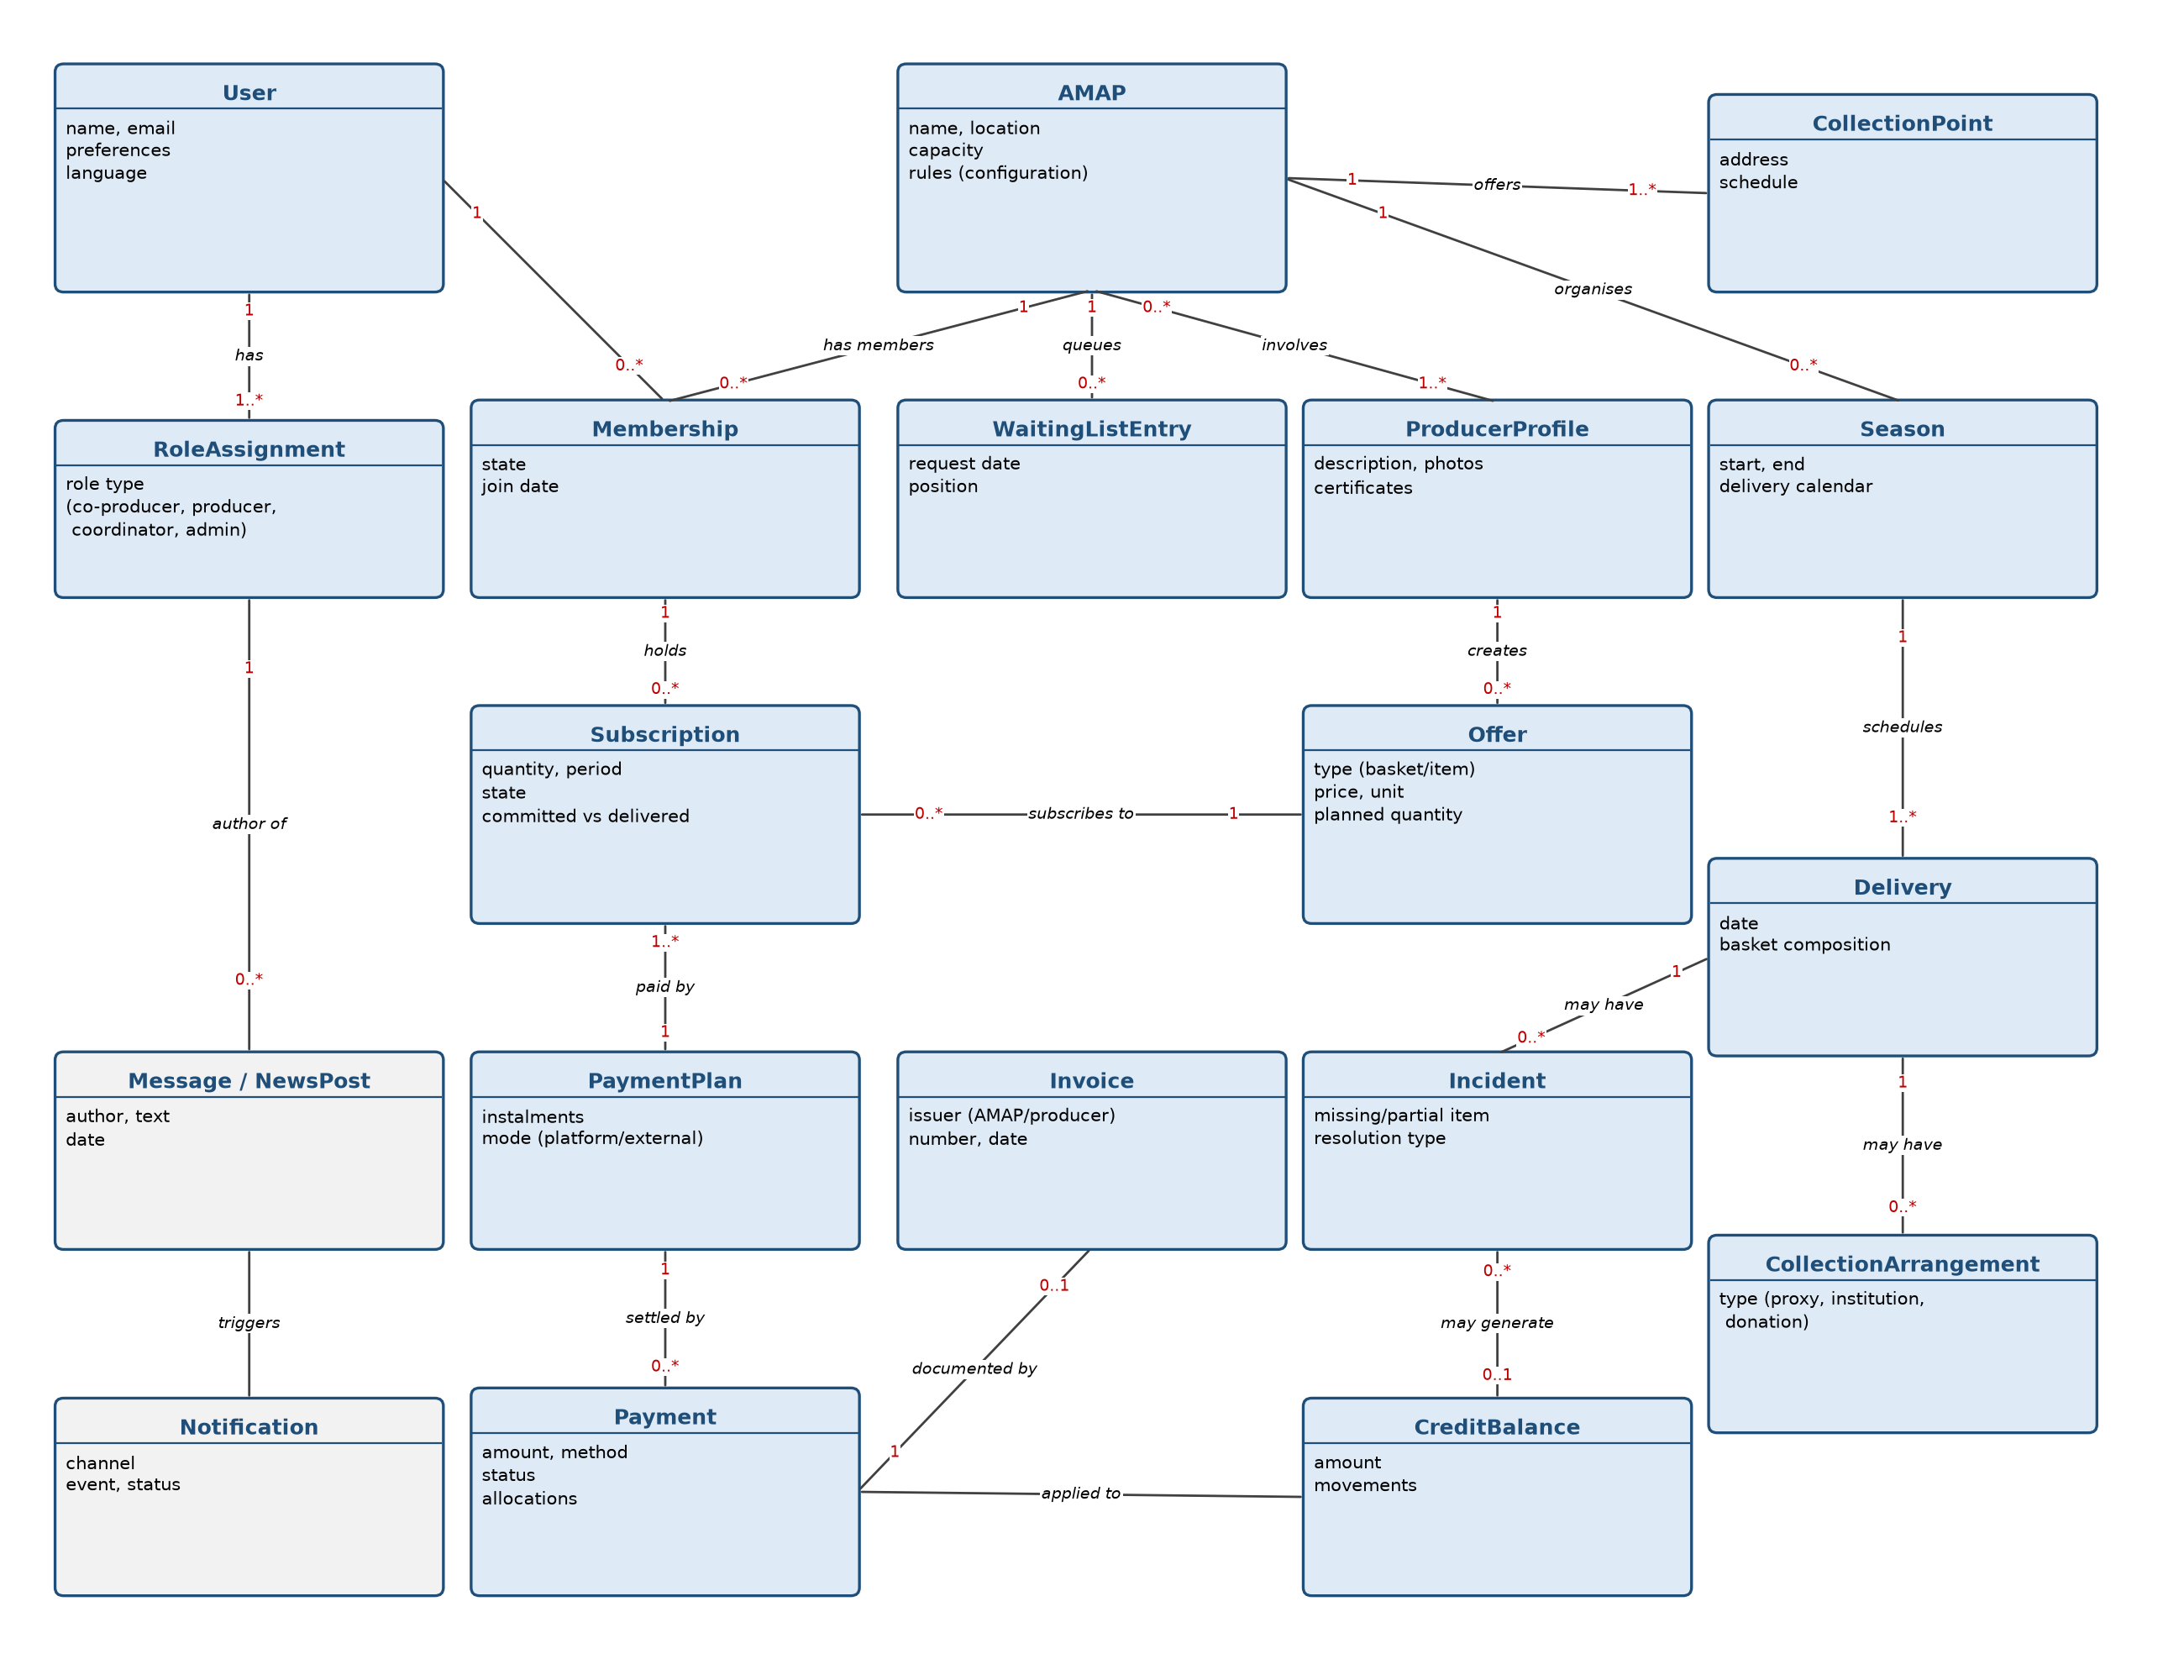
\includegraphics[width=1.00\linewidth]{figures/fig2_domain.png}
\caption{Extended domain model (all features)}\label{fig:fig2_domain}
\end{figure}
Figure \ref{fig:fig3_subscription_states} shows the life cycle of a subscription. It makes explicit the rule from S2-P3 that pauses and cancellations depend on coordinator approval: the member only moves the subscription to ``Pause/cancel requested'', and only the coordinator can move it to Paused or Cancelled. Renewal starts a new subscription for the next season (FR-27).

\begin{figure}[htbp]\centering
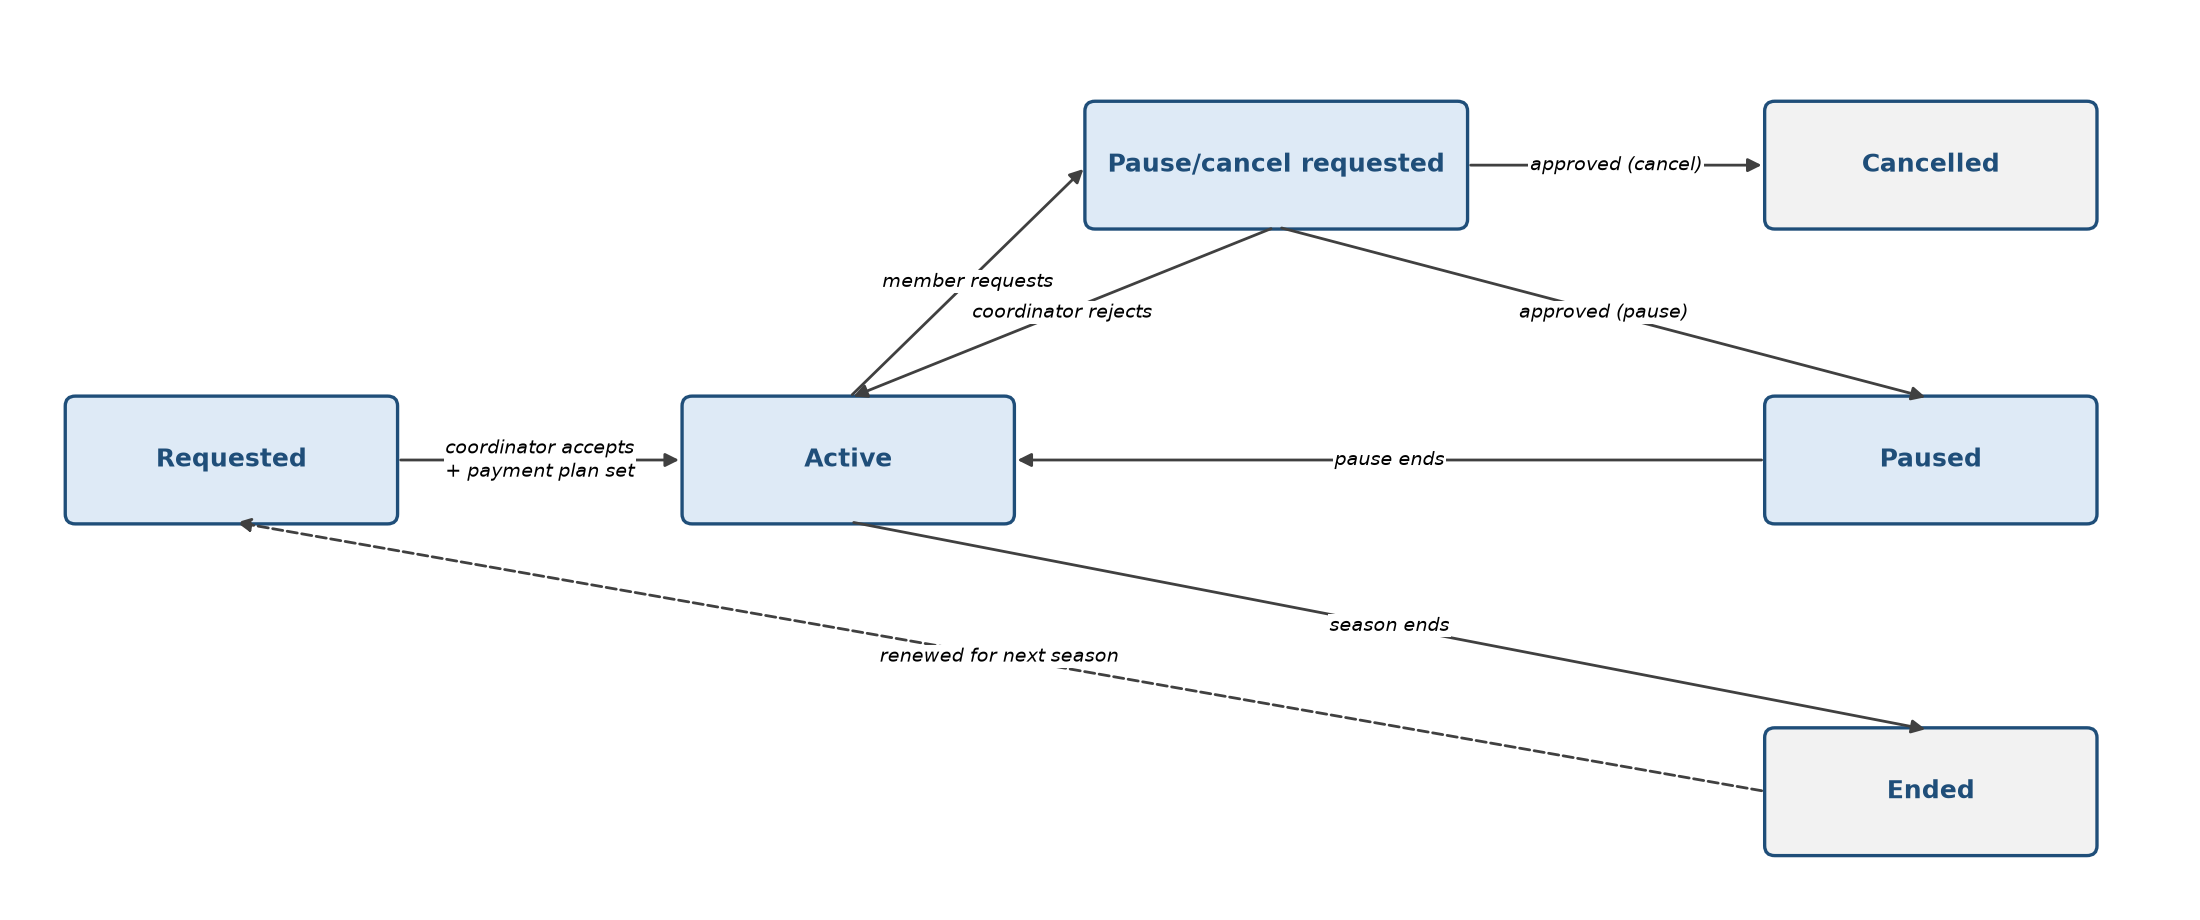
\includegraphics[width=0.97\linewidth]{figures/fig3_subscription_states.png}
\caption{Subscription state diagram}\label{fig:fig3_subscription_states}
\end{figure}

\subsection{Elicitation data detail}

The full raw notes are in the repository [R1]. Table \ref{tab:elicitation} summarises each question asked, the answer obtained and the requirements derived from it, providing the traceability from stakeholder statements to the specification.

{\footnotesize
\begin{longtable}{>{\raggedright\arraybackslash\hspace{0pt}}p{\dimexpr 0.085\linewidth-2\tabcolsep\relax}>{\raggedright\arraybackslash\hspace{0pt}}p{\dimexpr 0.218\linewidth-2\tabcolsep\relax}>{\raggedright\arraybackslash\hspace{0pt}}p{\dimexpr 0.461\linewidth-2\tabcolsep\relax}>{\raggedright\arraybackslash\hspace{0pt}}p{\dimexpr 0.236\linewidth-2\tabcolsep\relax}}
\caption{Elicitation questions, answers and derived requirements}\label{tab:elicitation}\\
\rowcolor{hdr}\textcolor{white}{\textbf{Ref.}} & \textcolor{white}{\textbf{Question (summary)}} & \textcolor{white}{\textbf{Answer (summary)}} & \textcolor{white}{\textbf{Derived}} \\ \endfirsthead
\rowcolor{hdr}\textcolor{white}{\textbf{Ref.}} & \textcolor{white}{\textbf{Question (summary)}} & \textcolor{white}{\textbf{Answer (summary)}} & \textcolor{white}{\textbf{Derived}} \\ \endhead
S1-Q1 & What should the software address? & Communication between producers and consumers; simpler payments; multiple producers and co-producers. & Scope, FR-41, FR-51 \\ \hline
S1-Q2 & User types and how it works & Several AMAP types with distinct rules; farmer creates offers and quantities; co-producer states product, quantity and period; advance orders; concepts Offer and Delivery. & FR-02, FR-16, FR-19, FR-21, FR-24, FR-25 \\ \hline
S1-Q3 & Monetisation and the AMAP spirit & Preference for a minimum fee per transaction and volume of co-producers; small producers start free or with a small rate. & FR-47, OR-01, OR-03 \\ \hline
S1-Q4 & Cycles & Seasonal cycles; produce dropped at a location; co-producers notified of the location. & FR-09, FR-29, FR-30 \\ \hline
S1-Q5 & Discovering and joining a CSA & Nearest CSA suggested; waiting list if no vacancies; co-producer subscribes to offers. & FR-06, FR-10, FR-12, FR-24 \\ \hline
S1-Q6 & Primary target audience & Streamline and energise the CSA market, not create CSAs; international; preference profile; two consumer types. & Scope, FR-04, NFR-O-03, LOC-03 to LOC-05 \\ \hline
S1-Q7 & Failures by producers or consumers & CSA management is important; abundance and scarcity cycles; balance by the end; news and communications. & FR-38, FR-51 \\ \hline
S1-Q8 & (not recorded) & No answer was given. & Open question \\ \hline
S1-Q9 & Quantifying sustainability & SDG aims; producers upload certificates or photos; KPIs nice to have. & FR-05, FR-23, FR-55 \\ \hline
S1-Q10 & Who issues the invoice? & Depends on the legal setup; avoid hundreds of individual payments. & FR-41, FR-48, FR-49 \\ \hline
S2-P1 & Payments and invoicing & Platform or external payments; one combined payment; money before delivery; each AMAP decides. & FR-40 to FR-42, FR-45 \\ \hline
S2-P2 & Shortages, missing products, quality & Producer chooses replacement, refund or credit (fox example). & FR-35 to FR-37, FR-39 \\ \hline
S2-P3 & Subscription changes & Cancel or pause only with AMAP management approval. & FR-26 \\ \hline
S2-P4 & Producer and coordinator responsibilities & Management decides the calendar; producers do not admit members. & FR-11, FR-17 \\ \hline
S2-P5 & Collection arrangements and notifications & Alternatives when absent; uncollected baskets not managed; notification one day before; identity check optional. & FR-31 to FR-34 \\ \hline
S2-P6 & Roles and internationalization & ``Does not matter.'' & FR-02 \\ \hline
S2-C1 & Payments and invoicing & One payment for all AMAPs, not the whole season; MB Way and transfer; PayPal and Apple Pay interesting. & FR-41, FR-43, FR-44 \\ \hline
S2-C2 & Seasonal variation and quality & Seasonal basket for most products; eggs, milk and bread chosen individually. & FR-20 \\ \hline
S2-C3 & Subscription flexibility & Informal resolution based on trust; in-platform chat useful. & FR-52 \\ \hline
S2-C4 & Membership and waiting lists & Explore an AMAP before joining; enrol in several AMAPs. & FR-03, FR-08 \\ \hline
S2-C5 & Collection and notifications & No answer recorded. & Open question \\ \hline
S2-C6 & Internationalization & Portuguese and English most important; other languages useful. & LOC-01, LOC-09 \\ \hline
S2-F & Additional findings & Geographic listing; AMAPs may communicate; payment mode per AMAP; several collection points. & FR-06, FR-09, FR-16, FR-53 \\ \hline
\end{longtable}}
Open questions still to be answered in the next sessions (from \url{docs/elicitation/open-questions}):

\begin{itemize}
  \item What are the problems of current AMAP/CSA software that amaply should solve?
  \item Which features are mandatory for the first release (MVP)?
  \item What volume of users and data is expected in the first year?
  \item Who pays, and what documents are involved in the end-to-end process?
  \item Is next season's production set by the farmer alone or agreed with the co-producers?
  \item Who issues the invoice in each legal setup and how should the system adapt?
\end{itemize}
\end{document}
